% This template was originally by R. Jacob Vogelstein
% Updated on March 1, 2010 by Noah J. Cowan


\documentclass[12pt,oneside,final]{thesis}\usepackage[]{graphicx}\usepackage[]{color}
%% maxwidth is the original width if it is less than linewidth
%% otherwise use linewidth (to make sure the graphics do not exceed the margin)
\makeatletter
\def\maxwidth{ %
  \ifdim\Gin@nat@width>\linewidth
    \linewidth
  \else
    \Gin@nat@width
  \fi
}
\makeatother

\definecolor{fgcolor}{rgb}{0.345, 0.345, 0.345}
\newcommand{\hlnum}[1]{\textcolor[rgb]{0.686,0.059,0.569}{#1}}%
\newcommand{\hlstr}[1]{\textcolor[rgb]{0.192,0.494,0.8}{#1}}%
\newcommand{\hlcom}[1]{\textcolor[rgb]{0.678,0.584,0.686}{\textit{#1}}}%
\newcommand{\hlopt}[1]{\textcolor[rgb]{0,0,0}{#1}}%
\newcommand{\hlstd}[1]{\textcolor[rgb]{0.345,0.345,0.345}{#1}}%
\newcommand{\hlkwa}[1]{\textcolor[rgb]{0.161,0.373,0.58}{\textbf{#1}}}%
\newcommand{\hlkwb}[1]{\textcolor[rgb]{0.69,0.353,0.396}{#1}}%
\newcommand{\hlkwc}[1]{\textcolor[rgb]{0.333,0.667,0.333}{#1}}%
\newcommand{\hlkwd}[1]{\textcolor[rgb]{0.737,0.353,0.396}{\textbf{#1}}}%

\usepackage{framed}
\makeatletter
\newenvironment{kframe}{%
 \def\at@end@of@kframe{}%
 \ifinner\ifhmode%
  \def\at@end@of@kframe{\end{minipage}}%
  \begin{minipage}{\columnwidth}%
 \fi\fi%
 \def\FrameCommand##1{\hskip\@totalleftmargin \hskip-\fboxsep
 \colorbox{shadecolor}{##1}\hskip-\fboxsep
     % There is no \\@totalrightmargin, so:
     \hskip-\linewidth \hskip-\@totalleftmargin \hskip\columnwidth}%
 \MakeFramed {\advance\hsize-\width
   \@totalleftmargin\z@ \linewidth\hsize
   \@setminipage}}%
 {\par\unskip\endMakeFramed%
 \at@end@of@kframe}
\makeatother

\definecolor{shadecolor}{rgb}{.97, .97, .97}
\definecolor{messagecolor}{rgb}{0, 0, 0}
\definecolor{warningcolor}{rgb}{1, 0, 1}
\definecolor{errorcolor}{rgb}{1, 0, 0}
\newenvironment{knitrout}{}{} % an empty environment to be redefined in TeX

\usepackage{alltt}

%\usepackage[utf8]{inputenc}
\usepackage{cite}

\usepackage{amssymb,amsmath,amsthm,amscd}
\usepackage{graphicx}
\usepackage{subcaption}

\usepackage{hyperref, mathrsfs, bm}
\usepackage{algorithm2e}
\usepackage{url}
\renewcommand{\thesubfigure}{}
% justifying
\usepackage{ragged2e}




\graphicspath{{./}{./graphs/}{./figures/}{./../JOFC-GraphMatch/graphs/}{./../JOFC_MatchDetect/graphs/}{./../SeededGraphMatch/graphs/}{./../DataFusion/}{./../DataFusion/graphs/}{./../DataFusion-graphmatch/graphs/}{./../VertexCorrespondence/graphs/}}

\usepackage{fixltx2e}
\usepackage{array}
% wrapfig is fragile: use sparingly
\usepackage{wrapfig} 
\usepackage{cmbright} %clean look
%\usepackage{times}  % Use this for ugly fonts
%\usepackage{ccfonts,eulervm} %Not bad looks nice for serif
\usepackage[T1]{fontenc}
\usepackage[latin1]{inputenc}

\usepackage{ogonek}
%\usepackage[garamond]{mathdesign}

\usepackage{verbatim}

\usepackage{multirow}

\usepackage{fancyhdr}    % Use nice looking headers along with the required footer page numbers   
%\usepackage[hypertex]{hyperref}
\usepackage{lscape} 
%Define the header/footer style
\pagestyle{fancy}
\fancyhf{}
\setlength{\headheight}{15pt}
\lhead{\leftmark}
\cfoot{\thepage}
\renewcommand{\headrulewidth}{0pt}
\fancypagestyle{plain}{% Redefine ``plain'' style for chapter boundaries
\fancyhf{} % clear all header and footer fields
\fancyfoot[C]{\thepage} % except the center
\renewcommand{\headrulewidth}{0pt}
\renewcommand{\footrulewidth}{0pt}}

\newtheorem{thm}{Theorem}
\newtheorem{cor}{Corollary}
\newtheorem{lem}{Lemma}

%\DeclareMathOperator*{\argmin}{arg\,min}

\newcommand{\myred}{\color{red}}
\newcommand{\mygreen}{\color{green!50!black}}
\newcommand{\myblue}{\color{blue}}

\newcommand{\mcX}{\mathcal{X}}
\newcommand{\mcY}{\mathcal{Y}}
\newcommand{\mcG}{\mathcal{G}}
\newcommand{\mcF}{\mathcal{F}}
\newcommand{\argmax}{\ensuremath{\arg\max}}
\newcommand{\argmin}{\ensuremath{\arg\min}}
\newcommand{\logodds}{\ensuremath{\mbox{log odds}}}
\newcommand{\Pos}{\ensuremath{\mbox{Pos}}}
\newcommand{\Neg}{\ensuremath{\mbox{Neg}}}
\newcommand{\Star}{\ensuremath{\mbox{star}}}
\newcommand{\Error}{\ensuremath{\mbox{Error}}}
\newcommand{\diag}{\ensuremath{\mbox{diag}}}
\newcommand{\degrees}{\ensuremath{\mbox{degrees}}}
\newcommand{\1}{\ensuremath{\mbox{{\bf 1}}}}
\newcommand{\Real}{\mathbb{R}}
\newcommand{\iid}{\stackrel{iid}{\sim}}


\newcommand{\mA}{\mathcal{A}}
\newcommand{\mD}{\mathcal{D}}
\newcommand{\mK}{\mathcal{K}}
\newcommand{\mC}{\mathcal{C}}
\newcommand{\mM}{\mathcal{M}}
\newcommand{\mN}{\mathcal{N}}
\newcommand{\mT}{\mathcal{T}}
\newcommand{\mI}{\mathcal{I}}
\newcommand{\mX}{\mathcal{X}}
\newcommand{\mY}{\mathcal{Y}}
\newcommand{\mZ}{\mathcal{Z}}
\newcommand{\mF}{\mathcal{F}}
\newcommand{\mP}{\mathcal{P}}


\newenvironment{remark}[1][Remark]{\begin{trivlist}
\item[\hskip \labelsep {\bfseries #1}]}{\end{trivlist}}



%\tolerance=10000

%\makeglossary % enable the glossary
\IfFileExists{upquote.sty}{\usepackage{upquote}}{}

\begin{document}





\title{Joint Optimization of Fidelity and Commensurability for Manifold Alignment and Graph Matching}
\author{Sancar Adali}
\degreemonth{May}
\degreeyear{2013} 
\dissertation
\doctorphilosophy
\copyrightnotice


% add your chapters, best way is to have separate TeX files for each chapter



%% FRONTMATTER
\begin{frontmatter}

% generate title
\maketitle

\begin{abstract}

Abstract goes here.

\vspace{1cm}

\noindent Primary Reader: Carey E Priebe\\
Secondary Reader: Daniel E Fishkind

\end{abstract}

\begin{acknowledgment}

Thanks!

\end{acknowledgment}

\begin{dedication}
 
This thesis is dedicated to \ldots

\end{dedication}

% generate table of contents
\tableofcontents

% generate list of tables
\listoftables

% generate list of figures
\listoffigures

\end{frontmatter}




\chapter{Introduction}
\label{sec:intro}
\chaptermark{Introduction:  Matched Data and Data Fusion}


Different views of the data

\section{Data Settings}


 It is a challenge  to do a tractable analysis on data from disparate sources of data (such as multiple sensors). The increasing multitude  of sensors technology and large numbers of sensors both are  sources of difficulty and hold promise for efficient inference. One of our contributions is developing well-defined simple settings that provided intuition for the right approaches to data fusion and which led to practically useful inference methods.
 
 Our world-view for data fusion of multiple sensors is depicted in \ref{fig:gen-model}.
 
\begin{figure}
\centering
\includegraphics[scale=0.75]{gen-model-orig-proj.pdf}
\caption{Multiple Sensor setting}
\label{fig:gen-model}
\end{figure}

It is assumed some objects lie in some "object`` space $\Xi$, and each sensor has another "view`` of the objects. The measurements recorded by the $i^{th}$ sensor lie in some "measurement space`` $\Xi_i$. The usual approach in pattern recognition is to use feature extractors on the spaces to get a feature representation in Euclidean space and use classical pattern recognition tools to carry out the exploitation task. The alternative approach is to acquire dissimilarities between the group of objects, and use the dissimilarities to either find an embedding in a low-dimensional Euclidean space where classic statistical tools are available for inference or use dissimilarity-based versions of pattern recognition tools~\cite{duin2005dissimilarity}. The embedding approach in a  low-dimensional Euclidean space will be used where the small number of embedding dimension allow us to avoid "curse of dimensionality``. Also, the embeddings of dissimilarities from  different conditions will be required to be "commensurate`` so that sensor measurements can be compared or jointly used in inference. This is accomplished by maps $\rho_k,k=1,\ldots,K$ from measurement spaces $\Xi_k$ to a low-dimensional commensurate space $\mathcal{X}$ visualized in~\ref{fig:gen-model}. Learning these maps from data is  an important portion of the proposed  approach.
\label{sec:data}

\subsection{Exploitation Task}
Data fusion is a very general concept and the specific meaning of data fusion and the setting we have in mind should be clarified here. The exploitation task we are interested in might involve (perhaps notional) complex objects or abstract entities that are not practically representable. The objects are members of a (perhaps notional) space called ``object'' space, $\Xi$ in Figure \ref{gen-model} . We will have different ``views'', ``measurements'' or ``data modalities'' extracted from these objects (which we will refer to as ``conditions''), and these observations will be elements of the measurement space for those ``conditions'' ($\Xi_k$ for $k^{th}$ condition). Each example of the objects will have an observation in each of the different conditions and the corresponding observations across different ``conditions'' will be ``matched''. Given new observations from these different ``conditions'', is it possible to decide if they are "matched``? Or if a group of  observations from each condition are "matched`` to each other, but the specific correspondences are unknown, is it possible to find the true correspondences? Different approaches are proposed in this dissertation to address these questions.
\label{subsec:task}



\section{Dissimilarity representation}
 Great progress been made in the theory and applications of pattern recognition, particularly in problem settings where the data available or assumed to be available as vectors in metric spaces. There are still many problems where due to the nature of setting, one only has access to dissimilarities or  proximities or distances between measurements or subjective assessment  of similarities of objects. We thus have a superficial distinction between these two kinds of settings, even though the inference task doesn't distinguish between this representation issue. The gap between the two kinds of representation of data can be bridged using various  techniques, such as different kinds of embedding methods and computing dissimilarities between entities.
We will refer to the entities of interest for pattern recognition as objects. These might be real objects or abstract concepts. The data will be a collection of measurements for instances or examples of these objects.
 \cite{Duin} is an excellent resource that compiles the fruits of research in learning from  dissimilarity-based representation. In the introduction, the authors make clear the distinction between statistical and structural(syntactic) pattern recognition, which is previously discussed in \cite{NadlerSmith1993}. The first is concerned with the analysis of features which are lists of measured values for object attributes. The second uses a relational view of objects for representation. In both cases,  the task of discrimination  can rely on distances (however they are defined). P\k{e}kalska and Duin  suggest dissimilarity measures  are a natural bridge between these two types of information and this applicability to  multiple settings motivates our use of dissimilarity representation in information fusion. 
For feature-based representation, one first defines the features which are either raw or processed measurements from sensors observing the objects and  represention of each object is a single point in the representation space. Dissimilarity-based representation relies on a dissimilarity measure, a way of quantifying the dissimilarity, proximity or similarity between any two objects. It is quite possible, in fact preferable, that the dissimilarity is \emph{designed for} the inference task at hand. 
%\cite{Duin} argue this is a reason dissimilarities can be superior, since similarities can encode concepts of class membership directly in class discrimination problems.
There are naturally multiple ways (some more natural than others) of comparing entities and this fact will provide one of the arguments for our approach to information fusion from  data sources, even sources that collect  data of same modality. In  the latter case where the data comes from separate sensors that are of the same type, the same measurements might have different dissimilarity representation according to subjective judgments or different dissimilarity  measures. 

\section{Match Detection}


For a formal description of the problem, consider $n$  $n$ distinct objects, which are described with finite number of measurements. Each of the measurements $x_{ik}$ lies in  the corresponding space $\Xi_k$ and the  measurements $x_{ik}$ are matched for the same $k$ index
\[  \begin{array}{cccc}
        & \Xi_1 & \cdots & \Xi_K\\
        Object ~ 1 & \bm{x}_{11} & \sim \cdots \sim & \bm{x}_{1K} \\
        \vdots & \vdots & \vdots & \vdots \\
        %\text{Object} ~ i & \bm{x}_{i1} & \sim \cdots \sim & \bm{x}_{iK} \\
        %\vdots & \vdots & \vdots & \vdots \\
        Object ~ n & \bm{x}_{n1} & \sim \cdots \sim & \bm{x}_{nK}
      \end{array}      
\]
To each pair of measurements $x_{ik},x_{jk}$ in the same space, we can assign a dissimilarity value $\delta_{ijk}=\delta\{x_{ik},x_{jk}\}$, possibly dependent on the space $\Xi_k$. We assume the dissimilarities to be non-negative and  symmetric, and 0 for $\delta\{x_{ik},x_{ik}\}$.  It is this training set of  dissimilarities we utilize to do inference on the following exploitation task:

 Given dissimilarities between  $K$ new measurements/observations ($\bm{y}_{k};k=1,\ldots,K$) and the previous $n$ objects under $K$ conditions, 
test the null hypothesis  that ``these measurements are from the same  object"  against the alternative hypothesis that ``they are not  from the same  object"~\cite{JOFC}:
    \[
\begin{array}{l}
%\hspace{-2em}
    H_0: \bm{y}_{1} \sim \bm{y}_{2} \sim \cdots \sim \bm{y}_{K}
 \text{ versus } 
 H_A: \exists i, j , 1\leq i < j \leq K :\bm{y}_{i} \nsim \bm{y}_{j}  
\end{array}
\]
 The null hypothesis can be restated as the case where the dissimilarities are ``matched" and the alternative as the case where they are not ``matched".

We represent the dissimilarities in the form  of $n \times n$  dissimilarity matrices $\{\Delta_k;k=1,\ldots,K\}$ with entries $\{\delta_{ijk} ;  i=1,\ldots,n;\quad j=1,\ldots,n\}$  and a  vector (of length $nK$) of dissimilarities  $\mathbf{\Delta}^{new}=\{ \delta_{ik}^{new}; i=1,\ldots, n;\quad k=1,\ldots,K\}  $  where $\delta_{ik}^{new} $ is the dissimilarity  between  $x_{ik}$ and $y_k$.
 

 
 
The inference task  is to find a collection of mappings (one from each ``condition'') to a lower dimensional space where new observations from each condition can be mapped to be made commensurate. These mappings does not need to be  well-defined; they can be the results of embedding routines for a particular dataset. As long as the embedding of the dissimilarity results in a  unique mapping,  out-of-sample embeddings could be adjoined to the embedding of in-sample dissimilarities.

A few points should be mentioned to distinguish our approach from related approaches.
 Due to the fact that data sources are ``disparate", it is not immediately obvious how  a dissimilarity between an object in one condition and another object in another condition  can be computed, or even defined.  In general, these between-condition between-object  similarities are not available.
 
 Whether the data is collected in dissimilarity representation for each condition, or whether dissimilarities are computed for the observations which are feature observations at each condition is not relevant to our exploitation task: it is assumed one way or another (perhaps from experts in the domain of the problem),  dissimilarities for each condition are available for inference purposes. 

The exploitation task  being considered is \emph{not} accurate reconstruction of these feature observations, even if they do exist. The quality of the  embeddings need to just be  good enough to be useful in the inference task. Therefore, the quality of our representation will be dependent on the bias-variance tradeoff, where by choosing a low-dimensional representation, we might be introducing more model bias, but the representation will be more  robust with respect to noise and might result in smaller error in the inference task.

We will make use of this inference problem for elucidating two concepts that we introduce  in \ref{chap:FidComm}.




\chapter{Related Work}
\label{sec:Related}
\chaptermark{Related Work}



\section{Multiple View Learning}
\label{sec:section}
When data are collected using a multitude of sensors or under significantly different environmental conditions, we refer to  the data setting as a multiple view setting where each ``view'' provide possibly complementary  information about the observed objects\footnote{We use the term ``object''  loosely, as the observed objects could be topics or concepts and the  collected data could be text, images, etc.}. Multiple view learning seeks to exploit these views simultaneously to be more successful in the learning task.

In data settings for multiview learning, the data consist of observations from $K>1$ views, where both the relationship between the attributes from different views and the relationship between the features and the quantity to be predicted are unknown. The objective is to train the best predictor. While it is possible to use all the attributes in different views and carry out feature selection without regards from which view they come from, this ignores the fact that the modalities can be quite diverse and combining features from different modalities is not always meaningful. Consider features extracted from an image  and an audio segment as features from different modalities. A classifier that treats these features in the same way without taking into consideration their modalities is  unlikely to have good performance.
It is more reasonable to use the prior information that the features in the same modality are much more likely to be correlated or commensurate with each other than features in different views and use predictors more suited to each modality, if the different modalities are diverse.

 Multiple View Learning is a burgeoning field, as there are many cases where one has to leverage many different related datasets for an inference task. For example, for learning  tasks related to webpages (such as webpage categorization, ranking of relevant webpages) both content of the webpages and the hyperlink structure between the webpages can be used. For social networks, people have different relationships with other people in their networks: networks  may be based on similarity of interests, geographical proximity, job relationships, etc. Combining information from different social networks would provide a more complete look into underlying social life of the people in the network and one would expect better performance in for all kinds of  inference based the social network data.

In addition, when it is necessary to collect more data, in a lot of cases it is easier to collect data in different modalities, than it is to collect more samples in a single modality. For example in medical studies, it is much easier to  collect medical data from already recruited patients, compared to recruiting new patients. Data from different modalities might provide complementary information and could result in much more effective predictors, as opposed to data from a single modality that provides diminishing returns with increasing sample size.

There are  also connections of this topic to well-studied machine learning subjects such as dimensionality reduction. As more data is collected, it is necessary to learn a low-dimensional representation of the data to avoid the curse of dimensionality. An interesting question is how to carry out dimensionality reduction in a multiple view setting: is it better to do dimensionality reduction separately for each modality, and concatenate the resulting low-dimensional representations, or find a joint low-dimensional representation  for all of the modalities? This is a question we try to answer for data settings we discuss in this thesis.

In the case of missing data, observations of features in the same view could  be missing altogether. In the case of such structurally missing data, it makes sense to learn predictors that use features from different views independently, so that a predictor could make an accurate prediction even if observations from some of the views are missing.


In  \cite{Amini2009}, the authors  discuss  an example of multiview learning problems, classification of a multi-lingual document corpus. They  co-train  classifiers for single-language data that jointly minimize  loss in each single language along with disagreement between classifiers on training examples. Their findings support the intuition that  classifiers which are based on multiview learning preform than those classifiers who have been trained with only data from a single view.


A popular approach to multiview learning is learning a  kernel matrix for each modality and combining these kernels in an optimal way (with respect to the inference task). For $K$ views, let $i^{th}$ datum for $k^{th}$ be represented $X_{ik},\quad i \in {1,\ldots n}, k \in \{ 1,\ldots, K \}$ . For the datum in the same view, let ${\mcK}_{k} = \left[ \mck_{k} (X_{ik},X_{jk}) \right] $ be the kernel matrix defined for that view.  Since any convex combination of the kernels $\sum{\alpha_k \mck_{k} } $ is also a kernel, it is possible to compute a joint kernel $\mck$ that use all of the multiview data by convexly combining this data. Assuming that a kernel can be defined for each view, the learning problem is  finding the optimal (for the inference task) coefficients $\alpha_k$ for each view. These parameters are usually estimated using training data. Denoting the optimal  $\alpha_k$ by  $\hat{\alpha}_k$,  $\hat{\mcK} = \sum_k{\hat{\alpha}_k \mcK_{k} }  =  \left[ \sum_k{\hat{\alpha}_k {\mck_k} (X_{ik},X_{jk})} \right] $.  Given a new datum $x$, the kernel function for each view, $\mck_{k}$ ,  along with $\hat{\alpha}_k$ is used to compute the inner product for the joint kernel. 
\[
{\mck}(x,.)= \sum{\hat{\alpha}_k {\mck_k} (x_{k},X_{ik})} 
\]

Many papers on ``Multiple Kernel Learning"   exist in the literature~\cite{McFee:2011:LMS:1953048.1953063,Lin2009,Lanckriet2004} which are reviewed in a comprehensive survey \cite{MKLSurvey}.
Choi et al.\ \cite{Choi:2008:MIM:1619995.1620064} use the Markov random walk interpretation of multiple kernel matrices to combine into one kernel matrix. \cite{ZhouBurges2007a} is another work that uses the random walk interpretation to deal with multiview data. The learning task in  \cite{ZhouBurges2007a} is spectral clustering with multiple graphs.

\section[Transfer Learning and Domain Adaptation]{Transfer Learning \label{sec:translearn}}

Methods which utilize training data in one domain  as auxiliary information for  learning  in another domain fall under the term ``transfer learning'' \cite{TransLearnSurvey}. Sometimes the source domain and the target domain are actually the same, but the distribution of the data is different , e.g. inherent difference between training and test data due to collection conditions. We call this phenomenon sample selection bias or covariance shift \cite{Zadrozny2004a,TransLearnSurvey}.

Let us clarify the differences between  these learning tasks.  Let $y$ denote the random variable for the class label  for classification or the dependent variable for regression and $X$ denote the random variates we will use for the learning task. We will  make use of  the common assumption that data is $\iid$.  
Suppose we have two domains  ${\mcD}_s$ and ${\mcD}_t$ where the training data and test data is collected from, respectively. These are called the source and target domains, respectively.
The training data $\left(X_i,y_i\right) \in {\mcD}_s$ and are drawn from the joint distribution $\Pry(X,y)$. 
The test data $\left({X'}_i,{y'}_i\right) \in {\mcD}_t$ and have the distribution $\Pry'(X,y)$.
The most general objective is to infer $\Pry'(X,y)$  given $\iid$ sample of $\left(X_i,y_i\right) \in {\mcD}_s$. 
The learning task is usually minimizing  $\argmin E[\ell\{y, \argmax_y{\hat{\Pry}'(y \| X) } \}]$  
where $\hat{\Pry}'(y \| X)$  is an approximation  $\Pry'(X,y)$ based on the training and the test data. Basically we require an inference method for the data distribution of the target domain   $\hat{\Pry}'(y \| X)$ that minimizes expected loss for prediction in the target domain.

In the classical supervised learning setting, the source and target domains are the same and  $\Pry(X,y)$ is assumed to be the same as $\Pry'(X,y)$. If the target domain is the same as the source domain, ${\mcD}_s={\mcD}_t=\mcD$, but $\Pry(X) \neq\Pry'(X)$ while $\Pry(y\|X) \approx \Pry'(y \| X)$, this is the \emph{covariate shift} problem.  When we cannot make either of the assumptions $\Pry(X) = \Pry'(X)$ or $\Pry(y\|X) = \Pry'(y \| X)$, we have the \emph{sample selection bias} problem \cite{Zadrozny2004a}.


 In some learning problems, the source and target domains are different ${\mcD}_s \neq {\mcD}_t$ and all or a considerable portion of  the labels $\{{y'}_i\}$  in $\left({X'}_i,{y'}_i\right) \in {\mcD}_t$ are missing. In this case, domain adaptation methods allow the exploitation of both the  data in the source domain $\{\left({X}_i,{y}_i\right)\}$ and the data in the target domain  $\{\left({X'}_i,.\right)\}$ to construct a good predictor for the target domain\cite{DaumeIII2006,Ben-David_Dom_Adapt2007,Ling2008,Pan2008a}.
Various ``domain adaptation'' approaches\cite{Pan2008a,LowRankSharedConceptChen2012a} assume existence of mappings to a common latent space ${\mcD}_{com}$,  $\Psi_s:{\mcD}_s \rightarrow {\mcD}_{com} $ and $\Psi_t:{\mcD}_t \rightarrow {\mcD}_{com}$ to a  such that the class conditional distributions $\Pry(\Psi_s(X) \|y) = \Pry(\Psi_t(X') \| y'=y)$. If these mappings can be inferred, then they can be used to predict $y'$ given $\Psi_t(X')$ even if no $\left({X'}_i,{y'}_i\right) \in {\mcD}_t$ pairs exist. 
%Other approaches infer a mapping from from the source domain to the target domain.

\section[Manifold Matching]{Manifold Alignment}
There have many efforts toward solving ``manifold alignment", which is a problem related to both our data fusion problem, and the transfer learning problem\ref{sec:translearn}. ``Manifold alignment" seeks to find correspondences between observations from different ``conditions". The setting that is most similar to ours is the semi-supervised setting, where a set of correspondences are given and the task is to find correspondences between a new set of points in each condition. In contrast, our hypothesis testing task is to determine whether any given pair of points is ``matched" or not. The proposed solutions follow a common approach in that they look for a common commensurate space such that the representations (possibly projections or embeddings) of the observations in the commensurate space match.

Note the similarity of the description problem to the latent space approach for domain adaptation. For both domain adaptation and manifold alignment, the objective is to find mappings to a  common space  so that the data in  one domain can be used for inference in the other domain.

Wang and Mahedavan~\cite{Wang2008} suggest an  approach that uses embedding followed by Procrustes Analysis to find a map to a commensurate space. Given a paired set of points, Procrustes Analysis~\cite{Sibson}, finds a transformation from one set of points to another in the same space that minimizes sum of squared distances, subject to some constraints on the transformation. In the case mentioned in \cite{Wang2008}, the paired set of points are corresponding low-dimensional embeddings of kernel matrices.   For the embedding step, they made the choice of using Laplacian Eigenmaps, though their algorithm allows for any appropriate embedding method.

 Zhai et al.~\cite{Zhai2010}  finds two projection matrices to minimize three terms in an energy function similar to our JOFC approach (see chapter \ref{chap:FidComm}). One of the terms is the \emph{correspondence preserving term} which is the sum of the squared distances between corresponding points and is analogous to our commensurability error term. The other two terms are \emph{manifold regularization terms} and consist of the reconstruction error for a Locally Linear Embedding of the projected points. These terms, analogous to fidelity, make sure the projections in the lower dimension retain the structure of the original points. For fidelity error terms in our setting, this is done by preserving dissimilarities. For manifold regularization terms, this is done by preserving the local neighborhood of points, such that close points are not mapped apart.
Ham and Lee\cite{HamLee2005a} solve the problem in semi-supervised setting by a similar approach, by minimizing a cost function of three terms, two terms for fidelity of embedding, one term of commensurability.
In another paper  the simultaneous embedding is written  as a single function  that combines Fidelity and Commensurability terms. By using Local Linear embedding,  they are able to formulate the embedding as a function of a $2n \times d$ configuration matrix, and a tradeoff parameter between \emph{inter-dataset} and \emph{intra-dataset error} (corresponding to commensurability and fidelity, respectively). This approach could be used as another tool for the investigation of JOFC.



Another approach is Three-way Multidimensional scaling\cite{3wayNMDS,borg+groenen:1997}.
 This approach assumes the  different ``conditions" of the data are linear transformations of a single configuration and aims to find this single configuration. For our setting, one would first embed the in-sample dissimilarities via the three-way MDS, which would give as the linear transformations that map from group configuration to individual configurations under each condition. This is followed by out-of-embedding the OOS dissimilarities, and use the inverse of the transformation matrices to find the out-of-sample embeddings with respect to the group configuration. Since the out-of-sample embeddings are commensurate, the test statistic can be computed as the distance between the OOS embeddings. 








\chapter{An expository problem for Multiview Learning : Match detection}
\label{sec:match detection}
\chaptermark{Match detection Task}

 We are interested in problems where the data sources are disparate and the inference task requires that the observations from  the different data sources  can be judged to be similar or dissimilar.
  
	Consider a collection of  English Wikipedia articles  and   French articles on the same topics. A pair of documents in different languages on the same topic are said to be ``matched". The ``matched'' wiki documents are  not necessarily direct translations of each other, so  we do not restrict ``matchedness'' to be a well-defined bijection between documents in different languages.
	%therefore the matchedness relation do not require  a bijection from the document space to another.
	However the matched ``documents''  provide examples of  ``similar"  observations coming from disparate sources, and we assume the training data consist of  a collection of ``matched'' documents.
	
  The inference task we consider is match detection, i.e. deciding whether a new English article and a new French article are on the same topic or not. While  a document in one language, say English, can be compared with other documents in English, a  French document  cannot be represented using the same features, therefore cannot be directly compared to English documents.  It is necessary   to derive a data representation  where the  documents from different languages can be compared (are commensurate).  %This data representation  should both preserve the high similarity of ``matched''  observations, the degree of  similarity of observations coming from the same source, and the dissimilarity of ``unmatched'' observations. 
	We will use a finite-dimensional Euclidean space for  this commensurate representation, where standard  statistical inference tools can be used.
  %It should also be parsimonius, so that it can be learned from data of limited  size.
	
     ``Disparate data''  means that  the observations are from  different ``conditions'', for example, the data might come from different type of sensors. Formally, the original data  reside in a heteregenous collection of  spaces.  In addition, the data might be structured and/or might reside in  infinite dimensional spaces. Therefore, it is possible that a feature representation of the data is not available or inference with such a representation is fraught with complications (e.g. feature selection, non-i.i.d. data, infinite-dimensional spaces). This motivates our  dissimilarity-centric approach. For an excellent resource on the usage of dissimilarities in pattern recognition, we refer the reader to the Pekalska and Duin book \cite{duin2005dissimilarity}.
		
		Since we proceed to inference starting from a dissimilarity representation of the data, our methodology may be applicable to any scenario in which multiple dissimilarity measures are available.  Some illustrative examples include:  pairs of images and their descriptive captions,  textual content  and  hyperlink graph
structure of  Wikipedia  articles, photographs take under different illumination conditions. In each case, we have an intuitive notion of ``matchedness'': for photographs take under different illumination conditions, ``matched'' means they are of the same person. For a collection of linked Wikipedia articles, the different ``conditions''  are  the textual content and hyperlink graph structure, ``matched'' means a text document and  a vertex  corresponds to the same Wikipedia article. 

 
The problem can be formally described as follows:


Let $(\Xi,\mcF,\mcP)$ be a probability space,
i.e., $\Xi$ is a sample space, $\mcF$ is a sigma-field,
and $\mcP$ is a probability measure.
Consider $K$ measurable spaces $\Xi_1,\cdots,\Xi_K$ 
and measurable maps $\pi_k:\Xi \to \Xi_k$.
Each $\pi_k$ induces a probability measure $\mcP_k$ on $\Xi_k$.
We wish to identify a measurable metric space $\mX$
(with distance function $d$)
and measurable maps $\rho_k: \Xi_k \to \mX$,
inducing probability measures $\widetilde{\mcP}_k$ on $\mX$,
so that for $[x_1,\cdots,x_K]' \in \Xi_1 \times \cdots \times \Xi_K$
we may evaluate distances $d(\rho_{k_1}(x_{k_1}),\rho_{k_2}(x_{k_2}))$ in $\mX$.


Given $\xi_1,\xi_2 \iid \mcP$ in $\Xi$,
%For any distinct $\xi_1,\xi_2 \in \Xi$,
we may reasonably hope that the random variable
$d(\rho_{k_1}\circ\pi_{k_1}(\xi_1),\rho_{k_2}\circ\pi_{k_2}(\xi_1))$
is stochastically smaller than the random variable
$d(\rho_{k_1}\circ\pi_{k_1}(\xi_1),\rho_{k_2}\circ\pi_{k_2}(\xi_2))$.
That is, matched measurements 
$\pi_{k_1}(\xi_1),\pi_{k_2}(\xi_1)$
representing a single point $\xi_1$ in $\Xi$
are mapped closer to each other than are
unmatched measurements 
$\pi_{k_1}(\xi_1),\pi_{k_2}(\xi_2)$
representing two different points in $\Xi$.
This property allows inference to proceed in the common representation space $\mX$.


As the inference proceeds from dissimilarities, we cannot make any observations about the object
 $\xi \in \Xi$,  and the measurements $x_k = \pi_k(\xi) \in \Xi_k$ cannot be represented directly. Furthermore, we do not have knowledge of the maps $\pi_k$.
 We have well defined dissimilarity measures
$\delta_k:\Xi_k \times \Xi_k \to \mathbb{R}_+ = [0,\infty)$
such that $\delta_k( \pi_k(\xi_1) , \pi_k(\xi_2) )$
represents the ``dissimilarity'' of outcomes $\xi_1$ and $\xi_2$
under map $\pi_k$.
The data we have  available consist of dissimilarities between a sample of $n$ objects using $\{\delta_k\}_{k=1,\ldots,K}$
We propose to use sample dissimilarities for matched data in the disparate spaces $\Xi_k$
to simultaneously learn maps $\rho_k$ which allow for a powerful test of matchedness
in the common representation space $\mX$.

 This setting is visualized in  Figure ~\ref{fig:multisensor}.

\begin{figure}
  \begin{center}
\includegraphics[scale=0.75]{gen-model-orig-proj.pdf}
 \caption{Maps $\pi_k$ induce disparate data spaces $\Xi_k$ from ``object space'' $\Xi$.
    Manifold matching involves using matched data $\{\bm{x}_{ik}\}$
    to simultaneously learn maps $\rho_1,\ldots,\rho_K$
    from disparate spaces 
    $\Xi_1,\ldots,\Xi_K$
  to a common ``representation space'' $\mX$, for subsequent inference.}\label{fig:mm}
  \end{center}
  \label{fig:multisensor}
\end{figure}








\begin{comment}
If the source of dissimilarities  are actually observations that are vectors in Euclidean space,  unless 
\begin{itemize}
\item the dissimilarity matrix is the Euclidean distance matrix of the original observations, and, 
\item the embedding dimension is greater or equal to the dimension of the original observations,
\end{itemize}
MDS with raw stress will not result in a perfect reconstruction  of the original observations. Note that the objective of the (joint) embedding is not \emph{perfect} reconstruction, but the best embedding for the exploitation task which is to test whether two sets of dissimilarities are ``matched". What is considered a ``good"'  representation will be dependent on how well the information in original dissimilarities that is relevant to the the match detection task is preserved. Fidelity and commensurability quantify this preservation of information.
\end{comment}


\section{Problem Description}
In the problem setting considered here,  $n$ different objects are measured under $K$ different conditions (corresponding  to, for example, $K$ different sensors). We assume we begin with dissimilarity measures. These will be represented in matrix form as $K$ $n \times n$ matrices $\{\Delta_k,k=1 ,\ldots,K\}$.  In addition, for each condition, dissimilarities between  a new object  and the previous 
$n$ objects $\{\mathcal{D}_k,k=1 ,\ldots,K\}$ are available. Under  the null hypothesis, ``these new dissimilarities represent a single \emph{new} object  compared to the previous $n$ objects'', measured under $K$ different conditions (the dissimilarities are matched). Under the alternative hypothesis, ``the dissimilarities $\{\mathcal{D}_k\}$ represent separate \emph{new} objects compared to the the previous $n$ objects''  measured under $K$ different conditions (the dissimilarities are unmatched)~\cite{JOFC}. %The test dissimilarities are referred to as  out-of-sample (OOS) dissimilarities. 

For the English-French Wikipedia  article example in the introduction,  dissimilarities between the new English article and $n$ other English articles $(\mathcal{D}_1)$ are available, and likewise for the new French article  and other $n$ French articles $(\mathcal{D}_2)$ \footnote{in addition to the dissimilarities between articles in the same language  ($\{\Delta_k\})$ }. The null hypothesis is that the new English and French articles are on the same topic, while the alternative hypothesis is that they are on different topics.

  In order to derive a data representation where dissimilarities from disparate sources ($\{\mathcal{D}_k\}$)  can be compared, the dissimilarities must be embedded in a commensurate metric space where the metric can be used to distinguish between ``matched'' and ``unmatched'' observations.


To embed multiple dissimilarities  $\{\Delta_k\}$  into a commensurate space, an omnibus dissimilarity matrix  $M$ \footnote{a $nk \times nk$ partitioned matrix whose diagonal blocks are given by $\{\Delta_k\}$ }  is constructed. Consider, for $K=2$,
 \begin{equation}
M=  \left[ \begin{array}{cc}
         \Delta_1 & L\\
        L^T  & \Delta_2 
     \end{array}  \right]     \label{omnibus} 
\end{equation} where $L$ is a matrix of imputed entries.   

\begin{remark}
For clarity of exposition,we will consider $K=2$; the generalization to $K>2$ is straightforward. 
\end{remark}

We define the commensurate space to be  $\mathbb{R}^d$, where the embedding dimension $d$ is pre-specified. The selection of $d$ -- model selection -- is  a task that requires much attention and is  beyond the scope of this article. Investigation of the effect of $d$ on testing performance will be pursued in a  subsequent paper.

 We use multidimensional scaling (MDS) \cite{borg+groenen:1997} to embed  the omnibus matrix in this  space, and obtain  a configuration of $2n$ embedded points $\{\hat{x}_{ik}; i=1,\ldots,n;k=1,2\}$ (which can be represented as $\hat{X}$, a $2n \times d$ matrix). The discrepancy between the interpoint distances of $\{\hat{x}_{ik}\}$ and the given dissimilarities in  $M$ is made as small  as possible (as measured by an objective function $\sigma(\widetilde{X})$ \footnote{$\sigma(\widetilde{X})$ implicitly depends on the omnibus dissimilarity matrix $M$}). In matrix form, $$ \hat{X}=\arg \min_{\tilde{X}} \sigma(\tilde{X}).$$ 
%This approach will be referred to as the Joint Optimization of Fidelity and Commensurability (JOFC) approach, for reasons that will be explained in \ref{sec:FidComm}. 

\begin{remark} 
We will use $x_{ik}$ to denote the --possibly notional--  observation  for the $i^{th}$ object in the $k^{th}$ condition, $\tilde{x}_{ik}$ to denote an argument of the objective function  and  $\hat{x}_{ik}$  to denote the $\arg\min$  of the objective function, which coordinates of the embedded point. The notation for matrices ($X,\tilde{X},\hat{X}$) follows the  same convention.
\end{remark}

  Given the omnibus matrix $M$ and the $2n \times d$ embedding configuration matrix $\hat{X}$ in the commensurate space, the out-of-sample extension~\cite{TrossetOOS} for MDS will be used to embed the test dissimilarities $\mathcal{D}_1$ and $\mathcal{D}_2$.  Once the test similarities are embedded as two points ($\hat{y}_{1},\hat{y}_{2}$) in  the commensurate space, it is possible to  compute the test statistic \[
\tau=d\left(\hat{y}_{1},\hat{y}_{2}\right)\label{teststat}
\] for the two ``objects'' represented by  $\mathcal{D}_1$ and $\mathcal{D}_2$.  For large values of $\tau$, the null hypothesis will be rejected. 
   If  dissimilarities between matched objects are smaller than dissimilarities between unmatched objects with large probability, and the embeddings preserve this stochastic ordering,  we could reasonably expect the test statistic to yield large  power. 
   
   

\section{Definition of  $w^{*}$}

\begin{remark}
In our notation, $(.)$  denotes  either $(m)$  or   $(u)$. In the former case, an expression refers to values under  ``matched'' hypothesis, in the latter, the expression refers to values under  ``unmatched''   hypothesis.
\end{remark}
Let us denote the test dissimilarities ($\mathcal{D}_1$, $\mathcal{D}_2$)  by  ($\mathcal{D}_1^{(m)}$, $\mathcal{D}_2^{(m)}$)  under the  ``matched'' hypothesis, and  by ($\mathcal{D}_1^{(u)}$, $\mathcal{D}_2^{(u)}$)  under the alternative. The out-of-sample embedding of ($\mathcal{D}_1^{(m)}$, $\mathcal{D}_2^{(m)}$) involves the  augmentation of  the omnibus matrix $M$, which consists of $n$ matched  pairs of dissimilarities,  with ($\mathcal{D}_1^{(m)}$, $\mathcal{D}_2^{(m)}$). The resulting augmented  $(2n+2)\times (2n+2)$ matrix  has the form:

 \begin{equation}
\Delta^{(m)}=  \left[ \begin{array}{cccc}
          \multicolumn{2}{c}{\multirow{2}{*}{\Huge{$M$}}} &  \mathcal{D}_1^{(m)} &\vec{\mathcal{D}}_{NA}\\
        & &  \vec{\mathcal{D}}_{NA}   & \mathcal{D}_2^{(m)} \\
  			\mathcal{D}_1^{(m)T} & \vec{\mathcal{D}}_{NA}^T  &  0 & \mathcal{D}_{NA} \\
         \vec{\mathcal{D}}_{NA}^T & \mathcal{D}_2^{(m)T} & \mathcal{D}_{NA} &0\\
     \end{array}  \right].     \label{aug_omnibus} 
\end{equation}  where
the scalar $\mathcal{D}_{NA}$ and    $\vec{\mathcal{D}}_{NA}$ (a vector of NAs that has length $n$)   represent dissimilarities that are not available. 
In our JOFC procedure, these unavailable entries in $\Delta^{(m)}$ are either imputed using other dissimilarities that are available, in the way described before equation \eqref{raw-stress}, or ignored in the embedding optimization. For a simpler  notation, let us assume it is the former case. Also note that $\Delta^{(u)}$  has the same form as $\Delta^{(m)}$ where $\mathcal{D}_k^{(m)}$ is replaced by $\mathcal{D}_k^{(u)}$.

We define the dissimilarity matrices \{$\Delta^{(m)},\Delta^{(u)}$\} to be  two matrix-valued random variables: $\Delta^{(m)}:\Omega \rightarrow \mathbf{M}_{(2n+2)\times (2n+2)} $ and  $\Delta^{(u)}:\Omega \rightarrow \mathbf{M}_{(2n+2)\times (2n+2)} $) for the appropriate sample  space $(\Omega)$.
\begin{remark}
Suppose the objects in $k^{th}$  condition  can be represented as points in a measurable space $\Xi_k$, and the dissimilarities in $k^{th}$ condition are given by  a dissimilarity measure $\delta_k$ acting on pairs of points in $\Xi_k$. Assume $\mathcal{P}_{(m)}$ is the joint probability distribution over matched objects, while the joint distribution of unmatched objects \{$k=1,\ldots,K$\}  is $\mathcal{P}_{(u)}$. Assuming the data are i.i.d., under the two hypotheses (``matched'' and ``unmatched'', respectively), the $n+1$ pairs of objects are governed  by the product distributions $\{\mathcal{P}_{(m)}\}^n \times \mathcal{P}_{(m)} $ and $\{\mathcal{P}_{(m)}\}^n \times \mathcal{P}_{(u)} $.  The distributions of $\Delta^{(m)}$ and $\Delta^{(u)}$ are the induced probability distributions of  these product distributions (induced by the  dissimilarity measure $\delta_k$ applied to  objects in $k^{th}$ condition \{$k=1,\ldots,K$\}).
\end{remark}


%is embedded in $d$-dimensional space with the constraint that the embedding of the first $2n$ points is the same as the embedding of $M$:


 We now consider the embedding of $\Delta^{(m)}$ and $\Delta^{(u)}$ with the criterion function  $\sigma_W(\widetilde{X}; \Delta^{(.)})$. The arguments of the function are  $\widetilde{X}= \left[
\begin{array}{c}
{\widetilde{\mathcal{T}}} \\
\widetilde{y}_{1}^{(.)} \\
\widetilde{y}_{2}^{(.)}
\end {array}
\right]$ where ${\widetilde{\mathcal{T}}}$ is the argument for the in-sample embedding of the first $n$ pairs of matched points, and
 $\{\widetilde{y}_{1}^{(.)} \}$ and $\{\widetilde{y}_{2}^{(.)} \}$ are the arguments for the embedding coordinates of the matched  or unmatched pair,
and the omnibus dissimilarity matrix $\Delta^{(.)}$ is equal to  $\Delta^{(m)}$  (or $\Delta^{(u)}$) for the embedding of the  matched (unmatched) pair. Note that we use the simple weighting scheme, so with a slight abuse of notation, we rewrite the criterion function as  $\sigma_w(\widetilde{X}; \Delta^{(.)})$ where $w$ is a scalar parameter.
The embedding coordinates for the matched or unmatched pair  ${\hat{y}_{1}^{(.)},\hat{y}_{2}^{(.)}}$ are given by
 \[
{\hat{y}_{1}^{(.)},\hat{y}_{2}^{(.)}}
=\argmin_{\widetilde{y}_{1}^{(.)}, \widetilde{y}_{2}^{(.)}}\left[\min_{\widetilde{\mathcal{T}}}
{\sigma_w\left(
\left[
\begin{array}{c}
{\widetilde{\mathcal{T}}} \\
\widetilde{y}_{1}^{(.)} \\
\widetilde{y}_{2}^{(.)}
\end {array}
\right]
,
\Delta^{(.)}
\right)
}
\right].
\]

\begin{remark}
 Note that the in-sample embedding of $\widetilde{\mathcal{T}}$ is necessary but irrelevant for the inference task, hence the minimization with respect to $\widetilde{\mathcal{T}}$ is denoted by  $\min$ instead $\argmin$. It can be considered as a nuisance paramater for our hypothesis testing.
\end{remark}
\begin{remark}
 Note also that  all of the random variables following the embedding, such as $\{\hat{y}_{k}^{(.)}\}\!$,  are dependent on $w$; for the sake of simplicity, this will  be suppressed in the notation. 
\end{remark}

 Under reasonable assumptions, the embeddings $\Delta^{(m)} \rightarrow  \{\hat{y}_{1}^{(m)},\hat{y}_{2}^{(m)}\!\}$  and $\Delta^{(u)}\rightarrow \{\hat{y}_{1}^{(u)} , \hat{y}_{2}^{(u)}\}$ are measurable maps for all $w \in (0,1)$ \cite{measurable_Niemiro1992}. Then, the distances between the embedded points are random variables and we can define the test statistic $\tau$ as $d(\hat{y}_{1}^{(m)},\hat{y}_{2}^{(m)})$ under the null hypothesis  and $d(\hat{y}_{1}^{(u)},\hat{y}_{2}^{(u)})$ under the alternative. Under the null hypothesis, the distribution of the statistic is governed by the distribution of $\hat{y}_{1}^{(m)}$ and $\hat{y}_{2}^{(m)}$; under the alternative it is governed by  the distribution of $\hat{y}_{1}^{(u)}$ and $\hat{y}_{2}^{(u)}$.

 Then, the statistical power as a function of $w$ is given by  \[\beta\left( w,\alpha\right)=1-F_{d \left(\hat{y}_{1}^{(u)},\hat{y}_{2}^{(u)}\right)} \left(F_{d\left(\hat{y}_{1}^{(m)},\hat{y}_{2}^{(m)}\right)}^{-1}(1-\alpha) \right)\] where $F_Y$ denotes  the   cumulative distribution function of  $Y$. The area under curve (AUC) measure  as a function of $w$ is defined as  
\begin{equation} 
AUC(w)=\int_{0}^{1}\! \beta\left( w,\alpha\right)\,\mathrm{d}\alpha \; . \label{AUC_def}
\end{equation} 
%\footnote{
Although we might care about optimal $w$ with respect to  $\beta\left( w,\alpha\right)$ (with a fixed Type I error rate $\alpha$),  it will be more convenient to define $w^*$ in terms of the AUC function.
%}

 Finally, define $$w^{*}=\arg\max_w{AUC\left( w\right)}. $$

 Some important questions about $w^*$ are  related to the nature of the AUC function.
While finding an analytical expression for the value of $w^*$ is intractable, an estimate $\hat{w}^*$  based on  estimates of $AUC(w)$ %$\beta_{\alpha}(w^*)$
 can be computed.  For the Gaussian setting described in  section \ref{subsec:GaussianSet}, a Monte Carlo simulation is performed  to find the estimate of $AUC(w)$ for different values of $w$.
% $\beta_{\alpha}\left( w\right)$  at various values of $\alpha$ , 
%which can be used to compute  values .

\subsection{Continuity of $AUC(\cdot)$} 
 Let $T_0(w)=d(\hat{y}_{1}^{{(m)}},\hat{y}_{2}^{{(m)}})$ and $T_a(w)=d(\hat{y}_{1}^{(u)},\hat{y}_{2}^{(u)})$ denote the value of the test statistic under null and alternative distributions  for the embedding with the simple weighting $w$.  %stochastic process whose sample path is  a function of $w$ where the randomness comes from $\Delta^{(m)}$, $\Delta^{(u)}$ and %$\mathcal{T}$ . 
%Consider $\beta_{\alpha}(\cdot)$ as a function of $w$, which can be written as $P\left[T_a(\cdot)>c_{\alpha}(\cdot)\right]$ where $c_{\alpha}(\cdot)$ is the critical value for level $\alpha$. Instead of  $\beta_{\alpha}(\cdot)$  
The AUC function can be written as $$AUC(w)=P\left[T_a(w)>T_0(w)\right]$$ where $T_a(\cdot)$ and $T_0(\cdot)$  can be regarded as  stochastic processes whose sample paths are functions  of $w$.  We will prove that $AUC(w)$ is continuous with respect to $w$.
% except at a finite number of points in $(0,1)$.
We start with this lemma from \cite{Raik1972}.

\begin{lem}
Let $z$ be a random variable. The functional $g(z;\gamma) = P\left[z \geq \gamma \right]$ is upper semi-continuous in probability with respect to $z$. Furthermore, if $P\left[z = \gamma \right]=0$, $g(z;\gamma)$ is continuous in probability with respect to $z$. \label{lemma_1}
\end{lem}

\begin{proof}
Suppose $z_n$ converges to $z$ in probability. Then by definition, for any  $\delta>0$ and  $\epsilon>0$, $\exists	N\in\mathbb{Z^+}$ such that for all   $n \geq N$ 
$$ Pr\left[\left|z_n-z\right| \geq \delta \right] \leq \epsilon.$$

 The functional  $g(z;\gamma)$ is  non-increasing with respect to $\gamma$. Therefore, for $\delta>0$, 
$g(z_n;\gamma) -g(z;\gamma) \geq g(z_n;\gamma) -g(z;\gamma-\delta) $. Furthermore, $g(z;\gamma)$ is left-continuous with respect to $\gamma$, so the difference between the two sides of the inequality can be made as small as desired.

\begin{eqnarray}
g(z_n;\gamma) - g(z;\gamma-\delta) & = &Pr\left[z_n\geq \gamma \right] -Pr\left[z \geq  \gamma - \delta \right] \label{prob_defn}\\
& \leq &  Pr\left[\{z_n \geq \gamma \} \backslash \{z \geq \gamma - \delta \} \right] \label{set_diff}\\
& \leq & Pr\left[\{\{z_n \geq \gamma \} \backslash \{z \geq \gamma - \delta \} \} \cap \{z_n \geq  z\} \right] \label{conjunct_with_set} \\
& =  & Pr\left[\{z_n - z \geq \delta \} \right] \leq \epsilon. \label{upper_semicont}
\end{eqnarray}
 
Since $\epsilon$ and $\delta$ are arbitrary,
 $ \limsup_{n \rightarrow \infty} ( {g(z_n;\gamma)}- g(z;\gamma) ) =  0$ for any $\delta>0, $ i.e. $g(z;\gamma)$ is upper semi-continuous.

By arguments  symmetric to  \eqref{prob_defn}-\eqref{upper_semicont}, we can show that

\begin{equation}
g_(z;\gamma+\delta) - g(z_n;\gamma) \leq \epsilon. \label{lower_semicont}
\end{equation}


In addition, assume that  $P\left[z = \gamma \right]=0$. Then, $g(z;\gamma)$ is also right-continuous with respect to $\gamma$. Therefore, 
$g(z_n;\gamma) -g(z;\gamma) \leq g(z_n;\gamma) -g(z;\gamma+\delta)$ and the difference between the two sides of the inequality can be made as small as possible. 
Along with \eqref{lower_semicont}, this means that

 \[ 
\liminf_{n \rightarrow \infty} ( {g(z_n;\gamma)}- g(z;\gamma) ) = 0. 
\] Therefore, $\lim_{n\rightarrow \infty}g(z_n;\gamma) = g(z;\gamma)$, i.e. $g(z;\gamma)$ is continuous in probability with respect to $z$.
\end{proof}

\begin{thm} \label{main_thm}
Let $T(w)$ be  a stochastic process indexed by $w$ in the interval (0,1). Assume  the process is continuous in probability  (stochastic continuity)   at $w=w_0$,  i.e.
\begin{equation} \forall a>0 \quad  \lim_{s \rightarrow w_0} Pr\left[\left|T(s)-T(w_0) \right| \geq a \right] = 0 
\end{equation}
for $ w_0\in (0,1)$. Furthermore, assume that $Pr\left[T(w_0)=0\right]=0$.

Then, $Pr \left[ T(w) \geq 0\right]$ is continuous at $w_0$.
\end{thm}

\begin{proof}
Consider any sequence $w_n \rightarrow w_0$. Let $z_n = T(w_n)$ and  $z=T(w_0)$ and choose $\gamma=0$. Since $T(w)$ is continuous in probability at $w_0$ and $Pr\left[T(w_0)=0\right]=0$, conditions for Lemma \ref{lemma_1} hold, i.e.\hspace{-.5em} as $w_n\rightarrow w_0$, $z_n$ converges in probability to $z=T(w_0)$. By  Lemma \ref{lemma_1}, we conclude  $g(T(w_n); 0 ) = Pr \left[ T(w_n) \geq 0\right]$ converges to $g(T(w_0);0)$. Therefore $g(T(w);0)$ is continuous with respect to $w$.
\end{proof}


\begin{cor}{
 If $Pr[T_a(w)-T_0(w)=0]=0$ and $T_a(w)$, $T_0(w)$ are continuous in probability for all $w \in (0,1)$, then $AUC(w)=Pr\left[T_a(w)-T_0(w) >0 \right]$ is continuous with respect to $w$  in the interval $(0,1)$.}
\end{cor}
\begin{proof}

Let $T(w)=T_a(w)-T_0(w).$ Then Theorem \ref{main_thm} applies everywhere in the interval (0,1).
\end{proof}

In any closed interval that is a subset of $(0,1)$, the AUC function is continuous and therefore attains its global maximum in that closed interval.

 We do not have closed-form expressions for the null and alternative distributions of the test statistic $\tau$ (as a function of  $w$), so we cannot provide a rigorous proof of the uniqueness of $w^*$. However, for various data settings, simulations \ref{sec:simexp_results} always resulted in \emph{unimodal}  estimates for the AUC function which indicates a unique $w^*$ value.






\chapter{Fidelity and Commensurability}
\label{chap:FidComm}
\chaptermark{Fidelity and Commensurability}

\section{The concepts of  Fidelity and Commensurability\label{chap:FidComm}}

For the sake of argument, assume that the source of dissimilarities  are actually observations that are vectors in Euclidean space. MDS with raw stress will not result in a perfect reconstruction  of the original observations, unless the two conditions are satisfied:
\begin{itemize}
\item the dissimilarity matrix is the Euclidean distance matrix of the original observations. 
\item the embedding dimension is greater or equal to the dimension of the original observations.
\end{itemize}
 Note that this point is not relevant to our work, as   the objective of the (joint) embedding is not \emph{perfect} reconstruction, but the best embedding for the inference task. What is considered a ``good''  representation will be dependent on how well the original dissimilarities that is relevant to the inference task are preserved. Fidelity and commensurability quantify this preservation of information.


Regardless of the inference task,  to expect reasonable performance from the embedded data in the commensurate space  for the inference task at hand, 
%we have to use both the original dissimilarity information in each separate condition \emph{and}  the matchedness of dissimilarities. 
it is necessary to pay heed to these two error criteria: %adhered to
\begin{itemize}
\item Fidelity describes how well the mapping to commensurate space preserves the original dissimilarities. The \emph{loss of fidelity} can be measured with the  within-condition \emph{ fidelity error}, given by
    \[
\epsilon_{f_{(k)}} = \frac{1}{{{n}\choose{2}}} \sum_{1 \leq i < j \leq n} (d(\widetilde{\bm{x}}_{ik},\widetilde{\bm{x}}_{jk})-\delta_{ijkk})^2
.\] 
Here $\delta_{ijkk}$ is the dissimilarity between the $i^{th}$ object and the $j^{th}$ object where both objects are in the $k^{th}$  condition, and $\widetilde{\bm{x}}_{ik}$ is the embedded representation of the $i^{th}$ object  for the $k^{th}$ condition;  $d(\cdot,\cdot)$ is the Euclidean distance function.

\item Commensurability describes how well the mapping to commensurate space preserves matchedness of matched observations. The \emph{loss of commensurability} can be measured by the between-condition {\em commensurability error} which is given by
    \[
\epsilon_{c_{(k_1,k_2)}} = \frac{1}{n} \sum_{1 \leq i \leq n;k_1 <k_2} (d(\widetilde{\bm{x}}_{ik_1},\widetilde{\bm{x}}_{ik_2})- { \delta_{iik_1k_2}})^2
\label{comm-error}
\]
 for conditions $k_1$ and $k_2$; $\delta_{iik_1k_2}$  is the dissimilarity between the $i^{th}$ object under  conditions   $k_1$ and  $k_2$. 
Although  the between-condition dissimilarities of the same object, ${ \delta_{iik_1k_2}}$, are not available,  it is reasonable to set these dissimilarities to $0$ for all $i,k_1,k_2$. These dissimilarities correspond to  diagonal  entries of the  submatrix $L$ in  the omnibus matrix  $M$ in equation \eqref{omnibus}. Setting these diagonal entries to $0$ forces matched observations to be embedded close to each other. \label{commens}  
\end{itemize}
 Due to the fact that data sources are ``disparate", it is not obvious how  a dissimilarity between an object in one condition and another object in another condition  can be computed or  defined in a sensible way. Although  the between-condition dissimilarities of the same object, ${ \delta_{iik_1k_2}}$, are not available,
it is reasonable to  ignore them in the embedding by setting the associated weights in the raw stress function to be 0 for the weighted raw stress criterion. These dissimilarities correspond to  diagonal  entries of the  submatrix $L$ in  the omnibus matrix  M in equation \eqref{omnibus}. Setting these diagonal entries to $0$ forces matched observations to be embedded close to each other.  It is possible that this choice for between-condition dissimilarities might not be optimal. 
 We prefer this choice to  restrict our attention to  the fidelity-commensurability tradeoff. An alternative solution would be to impute these dissimilarities using other available dissimilarities.
By imputing the between-condition dissimilarities of the same object as 0, the commensurability error  term becomes
  \[
\epsilon_{c_{k_1k_2}} = \frac{1}{n} \sum_{1 \leq i \leq n;k_1< k_2} (d(\widetilde{\bm{x}}_{ik_1},\widetilde{\bm{x}}_{ik_2})))^2
\]



While  the above expressions for  \emph{fidelity} and  \emph{commensurability} errors  are specific to the joint embedding of disparate dissimilarities, the concepts of fidelity and commensurability are  general enough to be applicable to other dimensionality reduction methods for data from disparate sources. 

 There is also between-condition {\em separability error} given by
    $$\epsilon_{s_{k_1k_2}} = \frac{1}{{{n}\choose{2}}} \sum_{1 \leq i < j \leq n;k_1 <k_2} (d(\widetilde{\bm{x}}_{ik_1},\widetilde{\bm{x}}_{jk_2})-{ \delta_{k_1k_2}}(\bm{x}_{ik_1},\bm{x}_{jk_2}))^2.$$ This error will be ignored herein, due to the fact that 
$\delta_{k_1k_2}(\bm{x}_{ik_1},\bm{x}_{jk_2})$ is not  available. Although it is possible to impute these dissimilarities, the optimal  imputation is an open question and ignoring these terms provides for investigation of simpler, still open questions.

Note that the omnibus embedding approach using any variant of MDS tries to jointly optimize fidelity and commensurability, by minimization of some measure of discrepancy between the given dissimilarities (which are either between-condition or within-condition dissimilarities) and the distances of the embedded configuration. This is most obvious in the  raw stress version of  MDS, since the individual terms can be separated according to whether they are contributing to  fidelity or  commensurability  error.

 Consider the weighted raw stress criterion $\sigma_{W}(\cdot)$ with a weighting matrix $W$, given in equation~\eqref{raw-stress}.
 The omnibus matrix $M$  is a partitioned matrix consisting of matrices from different conditions ($k={1,2}$),  the entries of the matrix will be indexed by 4-tuple ${i,j,k_1,k_2}$ which refers to the entry in the $i^{th}$ row and $j^{th}$ column of the submatrix in  the $k_1^{th}$  row partition and   $k_2^{th}$ column partition. For example, the entry ${M}_{2n,n}$ will have the indices $\{i,j,k_1,k_2\}=\{n,n,2,1\}$ in the new indexing scheme. $D(\cdot)$ and $W$, which are the same size as $M$, follow the same 4-tuple indexing. Then,
 
\begin{align}
\sigma_W(\cdot)  &= & &\sum_{i,j,k_1,k_2} {w_{ij{k_1}{k_2}}(d_{ij{k_1}{k_2}}(\cdot)-M_{ijk_1k_2})^2 } \notag\\
\hspace{3pt} &=& &\underbrace{\sum_{i=j,k_1<k_2}  {w_{ij{k_1}{k_2}}(d_{ij{k_1}{k_2}}(\cdot)-M_{ijk_1k_2})^2}}_{Commensurability}  \hspace{10pt}  &  + &\hspace{2.5em} \underbrace{\sum_{i<j,k_1=k_2}  {w_{ij{k_1}{k_2}}(d_{ij{k_1}{k_2}}(\cdot)-M_{ijk_1k_2})^2  }  } _{Fidelity}\notag\\
\hspace{3pt}&+&  &\underbrace{\sum_{i< j,k_1<k_2}  {w_{ij{k_1}{k_2}}(d_{ij{k_1}{k_2}}(\cdot)-M_{ijk_1k_2})^2  }  } _{Separability}\label{eq:FidCommSep}\hspace{10pt} .
\end{align}


\begin{comment}
\begin{eqnarray}{ccc}
\sigma_W(\cdot)\hspace{3pt}   &= &\sum_{i,j,k_1,k_2} {w_{ij{k_1}{k_2}}(d_{ij{k_1}{k_2}}(\cdot)-M_{ijk_1k_2})^2 } \notag\\
\hspace{3pt} &= &\underbrace{\sum_{i=j,k_1\neq k_2}  {w_{ij{k_1}{k_2}}(d_{ij{k_1}{k_2}}(\cdot)-M_{ijk_1k_2})^2}}_{Commensurability}  \hspace{10pt}  &  + & \underbrace{\sum_{i\neq j,k_1=k_2}  {w_{ij{k_1}{k_2}}(d_{ij{k_1}{k_2}}(\cdot)-M_{ijk_1k_2})^2  }  } _{Fidelity}\notag\\
\hspace{3pt}&+ &\underbrace{\sum_{i\neq j,k_1\neq k_2}  {w_{ij{k_1}{k_2}}(d_{ij{k_1}{k_2}}(\cdot)-M_{ijk_1k_2})^2  }  } _{Separability}\label{eq:FidCommSep2}\hspace{10pt} .
\end{eqnarray}
\end{comment}


Since ${ \delta_{k_1k_2}}(\bm{x}_{ik_1},\bm{x}_{ik_2}) $ are set to 0, the corresponding entries of $M$ in the commensurability terms will be 0.

Since    the separability error is ignored,  the weights for separability terms are chosen to be 0. This also means off-diagonal elements of $L$ in equation \eqref{omnibus} can be ignored. When separability terms are removed from equation \eqref{eq:FidCommSep}, the resulting equation  is a sum of fidelity and commensurability error terms:


\begin{align}
\sigma_W(\cdot)\hspace{3pt}   
\hspace{3pt}&=&\underbrace{\sum_{i=j,k_1< k_2}  {w_{ij{k_1}{k_2}}(d_{ij{k_1}{k_2}}(\cdot))^2}}_{Commensurability}  \hspace{10pt}  &  +&\underbrace{\sum_{i< j,k_1=k_2}  {w_{ij{k_1}{k_2}}(d_{ij{k_1}{k_2}}(\cdot)-M_{ijk_1k_2})^2  }  } _{Fidelity}\notag\label{eq:FidCommSep}\hspace{10pt} .
\end{align}

This motivates  referring to the omnibus embedding approach as Joint Optimization of Fidelity and Commensurabilty (JOFC).


\section{Fidelity and Commensurability Tradeoff}
 The weights in the raw stress function allow us to address the question of the optimal tradeoff of  fidelity and commensurability. Let $w \in (0,1)$. Setting the weights ($\{w_{ijk_1k_2}\}$)  for the commensurability  and fidelity  terms    to $w$ and $1-w$, respectively,  will allow us to control the relative importance of fidelity and commensurability terms in the objective function. Let us denote the raw stress function with these simple weights by $\sigma_w(\widetilde{X};M)$.  With simple weighting, when $w=0.5$, all terms in the objective function have the same weights. We will refer to this weighting scheme in the rest of this dissertation as \emph{uniform weighting}. The alternative scheme, $w \neq 0.5$, is called \emph{nonuniform weighting}.
The initial  expectation in the investigation of fidelity and commmensurability was that there is a $w^*$ that is optimal for the specific match detection task ($w$ value which results in the best power for hypothesis testing). In fact,  exploratory simulations presented in \ref{} confirm the power of the tests varies with varying $w$ and indicate the range where the optimal  $w^*$ lies, assuming it exists. We show $w$ exists under certain conditions for the match detection task. Although we cannot provide  a rigorous proof of the uniqueness of $w^*$, for various data settings, simulations in \ref{} always resulted in \emph{unimodal}  estimates for the AUC function which indicates a unique $w^*$ value.
Specifically,  for the match detection task, we provide evidence in \ref{} that  uniform weighting does not necessarily yield the best fidelity-commensurability tradeoff in terms of subsequent inference and one should consider non-uniform weighting for better performance in the inference task.

\section{Incommensurability phenomenon}

 We can define a Dirichlet product model
that is designed specifically to illustrate when and why {\em jofc} is superior to both {\it p}$\circ${\it m} and {\em cca}
in terms of fidelity and commensurability.

If $q$ is large with respect to the target dimensionality $m$,
then with high probability {\em cca} will identify a $m-$dimensional subspace in the ``noise'' simplex $S^q$ with spurious correlation.
This phenomenon requires only that $a>0$.
In this event, the out-of-sample embedding will produce arbitrary $\widetilde{\bm{y}}_1$ and $\widetilde{\bm{y}}_2$,
even under $H_0$.
Thus the null distribution of the test statistic will be inflated by these spurious correlations.
If the allowable Type I error level is smaller than the probability of inflation,
then the power of the {\em cca} method will be negatively affected.

If $a$ is small and $m \leq p$, then with high probability the $m-$dimensional subspaces identified by the MDS step
will come from the ``signal'' simplex $S^p$.
If $m<p$, then with positive probability, these two subspaces,
identified separately in {\it p}$\circ${\it m},
will be geometrically incommensurate (see Figure \ref{fig:incomm}).
Thus the null distribution of the test statistic will be inflated by these incommensurate cases.
If the allowable Type I error level $\alpha$ is smaller than the probability of inflation,
then the power of the {\it p}$\circ${\it m} method will be negatively affected.


\subsection{ A symmetric example}

The
  \begin{figure}
  \begin{center}
    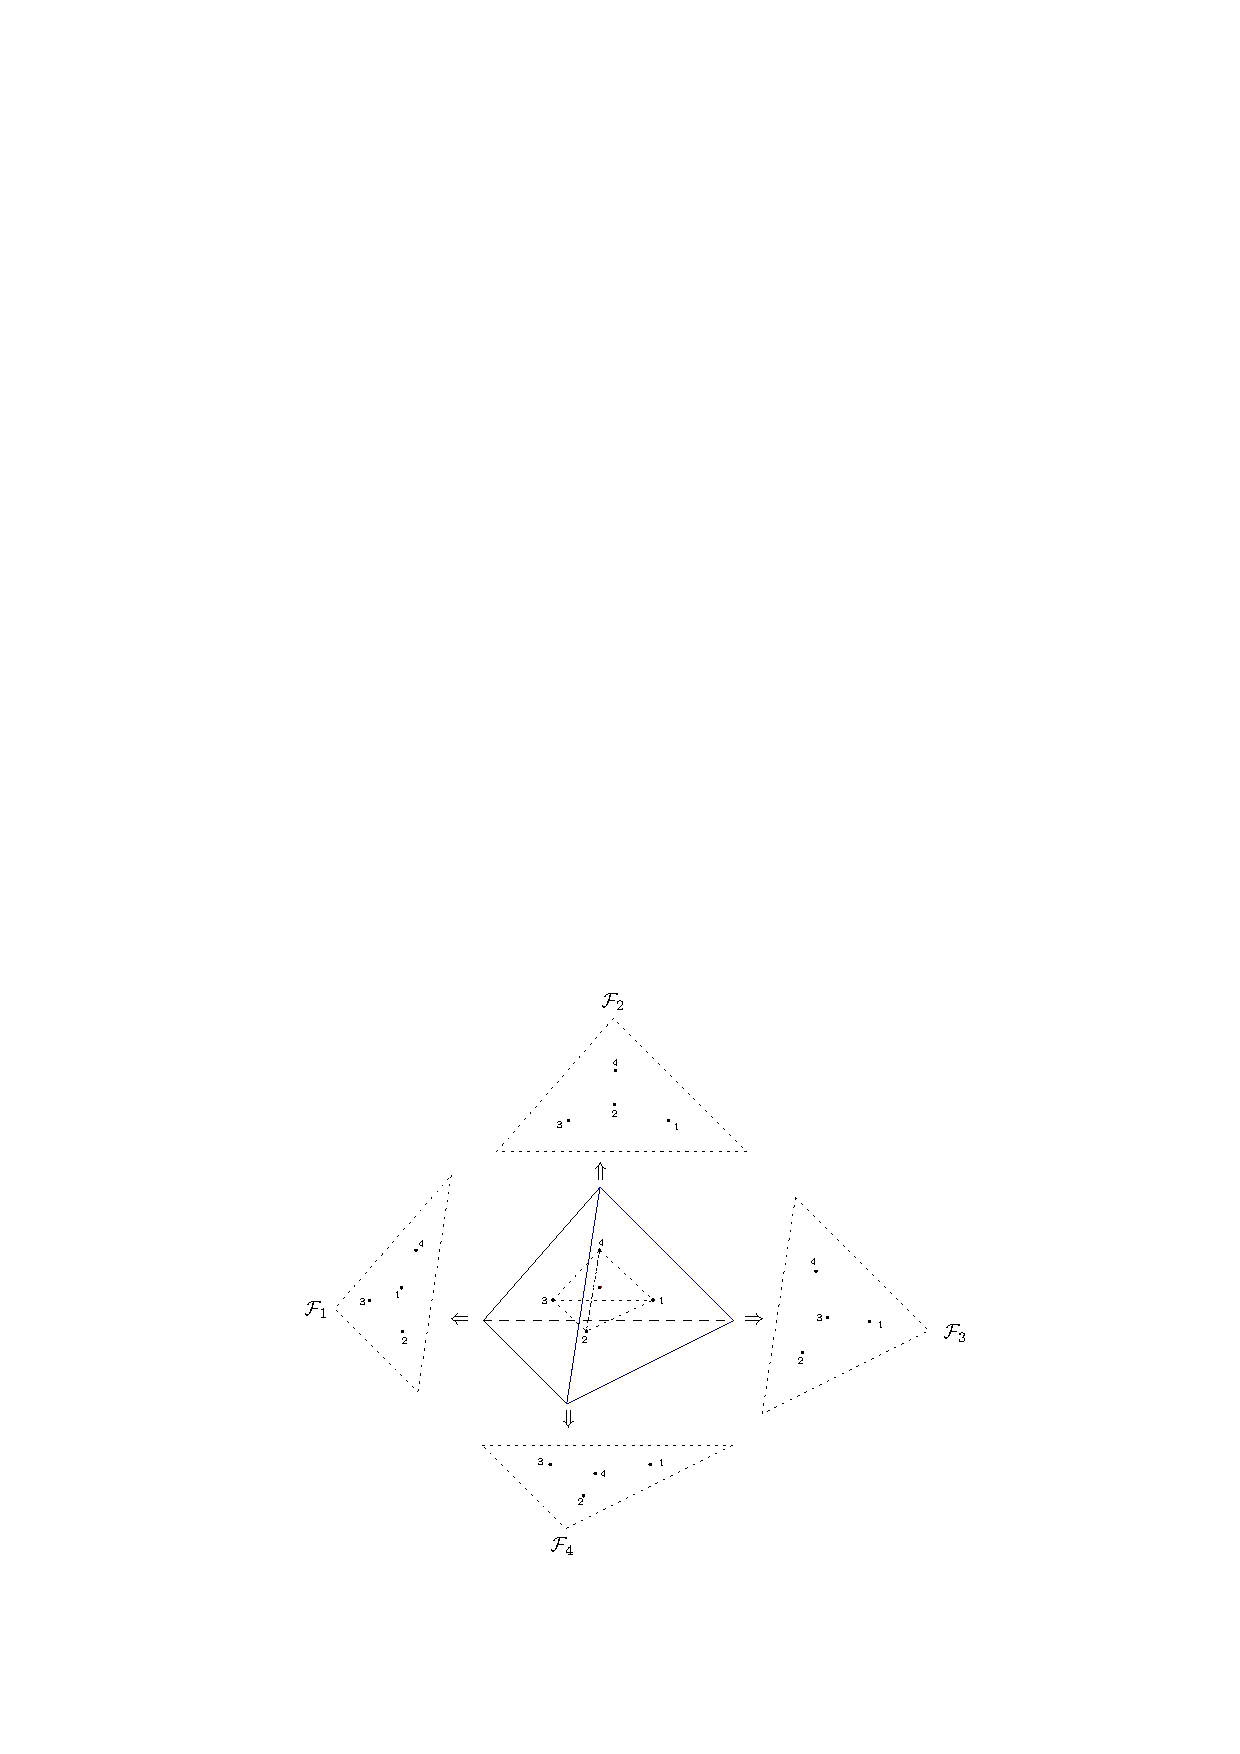
\includegraphics[height=13.2cm, width=15.84cm,angle=0]{ZMfacetprojections3d.pdf}
    \caption{Idealization of the incommensurability phenomenon:
    for a symmetric collection $\{\bm{\gamma}_1,\bm{\gamma}_2,\bm{\gamma}_3,\bm{\gamma}_4\}$ in the simplex $S^3$,
    all four of the facet projections have the same fidelity and are geometrically incommensurable with one another.}\label{fig:incomm}
  \end{center}
  \end{figure}

For large $q$ and small $a$, the two phenomena described above occur in the same model.
The {\it jofc} method is not susceptible to either phenomenon:
incorporating fidelity into the objective function obviates the spurious correlation phenomenon, and
incorporating commensurability into the objective function obviates the geometric incommensurability phenomenon.







\chapter{Procrustes Analysis on Low-dimensional Embeddings}
\label{sec:PoM}
\chaptermark{Procrustes Analysis}



\section{Procrustes Analysis}
Given two configurations of $n$ points in $d$-dimensional that include the same number of points,  and Procrustean methods try to fit one configuration to the other so that the points align as well as possible. Let us denote the configurations by two $n \times d$ matrices: ${\X}_1$, ${\X}_2$. The most general version of this  method  seeks an affine transformation $\rho$ from the configuration ${\X}_2$  to the target configuration ${\X}_1$  transformed by $\rho$ such that the sum of squares of the distances from each point transformed with $\rho$ to its corresponding point is minimized.
It is also possible to  enforce constraints on the affine transformation such as requiring the translation component to be a zero vector (if both of the point configurations are zero-centered), or setting the scaling component to 1 (if only rigid transformations are allowed). First let us consider the general case  $\rho({{\X}_2}) = s{\X}_2\mathbf{Q}+\1\mathbf{t}^T$ where $\mathbf{Q} \in \M_{d\times d}$, $s \in (0,\infty)$, $t\in \Real^{d}$. We will summarize the derivation of the components of the Procrustean transformation found in \cite{borg+groenen:1997}.

We seek to  minimize 
\begin{align*}
\mcL(s,\mathbf{Q},\mathbf{t}) &= \|{\X}_1 - (s{\X}_2\mathbf{Q}+\1 \mathbf{t}^T)\|_F^2  
\\ &= \tr {\left({\X}_1 - (s{\X}_2\mathbf{Q}+\1 \mathbf{t}^T) \right)^T \left({\X}_1 - (s{\X}_2\mathbf{Q}+\1 \mathbf{t}^T) \right)}.
\end{align*}

Setting the gradient $\frac{\partial \mcL}{\partial \bm{t}}=2 \left({\X}_1^T \1 - (s\mathbf{Q}^T {\X}_2^T \1+ n\mathbf{t})\right)$ to $\mathbf{0}$ ,
we solve for $\hat{\mathbf{t}}= n^{-1} \left({\X}_1^T \1  -s\mathbf{Q}^T {\X}_2^T \1 \right)$. 

Putting $\hat{\mathbf{t}}$ into  $\mcL(s,\mathbf{Q},{\mathbf{t}})$, we get 
\[\mcL(s,\mathbf{Q},\hat{\mathbf{t}}) = \tr \left((\bm{I}_n- \frac{\1 {\1} ^T}{n}){\X}_1 - (s{\X}_2\mathbf{Q} )\right)^T \left((\bm{I}_n- \frac{\1 {\1} ^T}{n}){\X}_1 - (s{\X}_2\mathbf{Q})\right).\]
Let us denote the centering matrix $\left(\bm{I}_n- \frac{\1 {\1} ^T}{n}\right)$  with $\bm{J}$. 
Setting  $\frac{\partial \mcL}{\partial s}=2 \tr {s{{\X}_2}^T  \bm{J} {{\X}_2}}-2 \tr {  {{\X}_1}^T \bm{J} {\X}_2\mathbf{Q}}=\bm{0}$,
we get $\hat{s}=\frac{ \tr {  {{\X}_1}^T \bm{J} {\X}_2\mathbf{Q}}}{\tr {{{\X}_2}^T  \bm{J} {{\X}_2}}}$.
Putting $\hat{s}$ into $\mcL(s,\mathbf{Q},\hat{\mathbf{t}})$, we get
$\mcL(\hat{s},\mathbf{Q},\hat{\mathbf{t}}) = 
\tr{{\X}_1^T \bm{J} {\X}_1}- 
\frac{ \left({ \tr{  {\X}_1^T \bm{J} {\X}_2\mathbf{Q} }}\right)^2}
{\tr{{\X}_2^T \bm{J} {\X}_2}} $.
The final step is computing the $\mathbf{Q}$. 
Note that the only term in $\mcL(\hat{s},\mathbf{Q},\hat{\mathbf{t}})$  that depends on $\mathbf{Q}$ is  $\tr \left( {\X}_1^T \bm{J} {\X}_2\mathbf{Q}\right)^2$. 
Subject to $\mathbf{Q}\mathbf{Q}^T=\mathbf{Q}^T\mathbf{Q}=\bm{I}_n$, minimizing   $- \left( \tr \left( {\X}_1^T \bm{J} {\X}_2\mathbf{Q}\right)\right)^2$ is equivalent to minimizing  $-\tr \left( {\X}_1^T \bm{J} {\X}_2\mathbf{Q}\right)$ (Since $\hat{s}>0$, minimizing $-x$ is the same as minimizing $-x^2$ given a constraint on $x$). So  \[\hat{\mathbf{Q}}=\argmin_{Q^TQ = \bm{I}_n}{-\tr \left( {\X}_1^T \bm{J} {\X}_2\mathbf{Q}\right)} \label{q_procrustes}\]. The solution for $\mathbf{Q}$ is equivalent to the solution of the orthogonal Procrustes problem.

For the orthogonal Procrustes problem, we seek  an orthonormal matrix $\mathbf{Q}^*$ that minimizes the sum of squared distances between the  target configuration ${\X}_1$ and  the configuration ${\X}_2$ transformed by $\mathbf{Q}^*$, i.e.,
 $\left[\mathbf{Q}^* = \argmin_{\mathbf{Q}^T\mathbf{Q} = \bm{I}_n} \|{\X}_1 - {\X}_2\mathbf{Q}\|_F  \right] $
 where $\|\cdot\|_F$ is the Frobenius norm on matrices.
Simplifying the norm expression, we get $\|{\X}_1 - {\X}_2\mathbf{Q}\|_F^2 = \tr {({\X}_1 - {\X}_2\mathbf{Q})^T({\X}_1 - {\X}_2\mathbf{Q})}= \tr {({\X}_1^T{\X}_1 + {\X}_2^T{\X}_2)} - 2\tr{ ({\X}_1^T {\X}_2\mathbf{Q})}$. Since the first term is independent of $\mathbf{Q}$, we can ignore that term. The second term  is equivalent to \eqref{q_procrustes} when  ${\X}_1^T\1 =  {\X}_2^T\1=\bm{0}$. The solution for $\mathbf{Q}^*$ is then the  $d\times d$ orthogonal matrix that maximizes $\tr{ ({\X}_1^T {\X}_2\mathbf{Q})}$.

 Consider the singular value decomposition $\mathbf{{\X}_1^T {\X}_2}=\bm{U} \bm{\Sigma} \bm{V}^T$. The expression to be minimized can be written as $\tr {\bm{U} \bm{\Sigma} \bm{V}^T \mathbf{Q}}$ which is equal to  $[\tr { \bm{V}^T \mathbf{Q} \bm{U} \bm{\Sigma}} $ due to circular invariancy of the trace operation.
 
 Note that for an orthogonal matrix $T\in \M$ and a diagonal matrix $\Lambda \in \M$ with non-negative entries $\Lambda_{ii}\geq 0$
 \[
 \tr{ T \Lambda } \geq \tr{ \Lambda} \] with equality if $T=\bm{I}$.
 
 Note $\bm{\Sigma}$ is diagonal with nonnegative entries  and $\bm{Z}=\bm{V}^T \mathbf{Q} \bm{U}$ is also orthogonal. To see why $\bm{Z}$ is orthogonal, consider 
 \begin{align*}
 \bm{Z}\bm{Z}^T &= \bm{V}^T \mathbf{Q} \bm{U} \bm{U}^T \mathbf{Q}^T  \bm{V} \\
 &= \bm{V}^T \mathbf{Q} \bm{I}_n \mathbf{Q}^T  \bm{V}\\
 &= \bm{V}^T \bm{I}_n  \bm{V} \\
 &= \bm{I}_n
 \end{align*} 
 each step justified by the fact that the SVD of $\mathbf{{\X}_1^T {\X}_2}$ results in matrices  $U$ and $V$ with orthogonal columns and $R$ is already known to be orthogonal.
 Therefore  $\tr { \bm{V}^T \mathbf{Q} \bm{U} \bm{\Sigma}}  \leq \tr \bm{\Sigma}$ 
with equality if  $\bm{V}^T \mathbf{Q} \bm{U} = I$ . So the solution  that achieves the bound is $\hat{\mathbf{Q}}= \bm{V}^T  \bm{U}$

\section{Procrustes Analysis for Manifold Matching}

Since separate  condition dissimilarities are available, a straightforward approach is to embed each conditional dissimilarity matrix, $\Delta_1$ and $\Delta_2$, separately  in  $d$-dimensional Euclidean space (call these embedded configurations ${\X}_1$ and ${\X}_2$, respectively) and then find a mapping function $\rho :\mathbb{R}^{d}\rightarrow\mathbb{R}^{d}$ that maps each point in ${\X}_2$ to approximately its corresponding point in ${\X}_1$. This approach can be seen as a specific example of the general setting where the commensurate space is d-dimensional  Euclidean space and $\rho_1$ in  ~\ref{fig:fig1} is the identity map. 

Estimation of $\rho$ is carried out using  Procrustes Analysis  on training data. Procrustes Analysis~The map $\rho$ estimated by the linear map $\mathbf{Q}^*$   makes the separate MDS embeddings as commensurate as possible. Once such a mapping is computed, one can out-of-sample embed  new dissimilarities for each condition (separately)  and  use $\mathbf{Q}^*$ to make the embeddings commensurate.
One can then compute the test statistic $\tau$ (the distance between commensurate embeddings) for  the hypothesis testing problem. This approach will be referred to  as P$\circ$M - Procrustes $\circ$ MDS.

Note that the Procrustes transformation $\mathbf{Q}^*$  is limited to  a linear transformation consisting of rotation and reflection and possibly also scaling components. The optimal mapping might  very well be   non-linear. If a larger class of mappings is considered, this would result in a smaller model bias but also larger variability for the mapping function. By only considering the class of linear transformations, it is possible to learn $\mathbf{Q}^{*}$ with the limited sample size.

\subsection{Relation of $P\circ M$ and Joint Optimization of Fidelity and Commensurability} 

Suppose the weights are chosen to be $w_{ijk_1k_2}=w$ for commensurability terms and $w_{ijk_1k_2}=1-w$ for fidelity terms in equation \eqref{eq:FidCommSep}. For the resulting weight matrix $W$, define 
\begin{equation}
f_w(D(\cdot),M) = \sigma_W(\cdot) \label{fid-comm-tradeoff-func}
\end{equation}
 where $M$ is the omnibus matrix obtained from  a given pair of dissimilarity matrices, $\Delta_1$ and $\Delta_2$, as in equation \eqref{omnibus}.   As $w$ goes to 0, the configuration embedded by JOFC converges to a configuration equivalent to (up to rotation and reflection)  the configuration embedded by P$\circ$M.


\begin{thm}
Define $\sigma(\cdot)=\sigma_{W=\bm{1}}(\cdot)$ (unweighted raw stress) where $\bm{1}$ is a matrix of 1's.
 Let $\mathbf{X}_1$ and $\mathbf{X}_2$ be the corresponding $n\times p$ configuration matrices with column means of $\bm{0}$ (obtained from separately embedding  $\Delta_1$ and $\Delta_2$ by minimizing the raw stress $\sigma(\cdot)$ ). 
Let  $\mathbf{Q}=\argmin_{\mathbf{P^T}\mathbf{P}=\mathbf{P}\mathbf{P^T}=\mathbf{I}}||{\mathbf{X}_1-\mathbf{X}_2}\mathbf{P}||^2$ ,   $\mathbf{\tilde{X}}_2= \mathbf{X}_2\mathbf{Q}$, 
and let  
$\mathbf{X}=\left[\begin{array}{c}
\mathbf{X}_1\\
\mathbf{\tilde{X}}_2
\end{array}\right]$.

For $w>0$, let $\mathbf{Y}_{w} = \left[\begin{array}{c}
\mathbf{Y}_1\\
\mathbf{Y}_2
\end{array}\right]$  be  a $2n \times p$ configuration matrix obtained by minimization of 
$ f(\mcY, M) =(1-w)\left({\sigma{(\mcY_1)}}+{\sigma{(\mcY_2)}}\right)+w||{\mcY_1-\mcY_2}||^2 $ with respect to  $\mcY=\left[\begin{array}{c}
\mcY_1\\
\mcY_2
\end{array}\right]$ with the constraint that $\mcY_1$ and $\mcY_2$ are two $n \times p$ configuration matrices having column means of $\bm{0}$. Then, $$lim_{w\rightarrow0}\mathbf{Y}_{w}=\mathbf{X}\mathbf{R}$$ for a $p\times p$ orthonormal matrix $\mathbf{R}$. ($\mathbf{R}$ is a transformation matrix with a rotation and possibly a reflection component.)
\end{thm}
 
\section{Generalized Procrustes Analysis ($K>2$)}
Generalized Procrustes analysis is the extension of Procrustes analysis to more than two configuration of points. This extension has been studied in \cite{GPCA}.






\chapter{Canonical Correlation Analysis for Data Fusion}
\label{sec:CCA}
\chaptermark{Canonical Correlation Analysis for Data Fusion}

For the CCA approach, MDS is used  to compute embedding configurations, $ X_1$ and $X_2$. It is desirable to  embed into the highest dimensional space  possible ($\mathbb{R}^{d'}$ where $d'=p+q$ for the Gaussian and Dirichlet settings)  to  preserve as many of the signal dimensions as possible (at the risk of possibly including  some noise dimensions). CCA~\cite{Hardoon2004}, then,  yields two mappings $\mathcal{U}_1$ and $\mathcal{U}_2$ that map these embeddings in $\mathbb{R}^{d'}$ to  the low-dimensional commensurate space ($\mathbb{R}^d$). 
While embedding the dissimilarities in the the highest dimension possible is a good idea for preserving the signal dimensions, in the presence of noise dimensions, the noise will be incorporated into the embeddings. Even if the dissimilarities are errorless representations of measurements of a particular dimension; for  the  sake of inference, it is preferable to embed at a lower  dimension due to the bias-variance tradeoff. This variant of CCA approach, which is called regularized CCA, with the  embedding dimension choice $d'< (p+q)$ is expected to have performance better than CCA approach.

\subsubsection*{Canonical Correlational Analysis}

 Let $X$ and $Y$ be two $s$-dimensional random vectors. If  one wants to find  the pair of linear projection operators $U_1:\mathbb{R}^s \rightarrow  \mathbb{R}$, $U_2 :\mathbb{R}^s \rightarrow  \mathbb{R}$ that maximize correlation between the projections of   $X$ and $Y$, CCA finds the solution as stated in the  optimization problem
$$
{\hat{(u)}_1 ,\hat{(u)}_2}=\arg\max_{u_1\in\mathbb{R}^s,u_2\in\mathbb{R}^s} {\frac{E[u_1^{T}XY^Tu_2]}{{E[u_1^{T}XX^T u_1]}{E[u_2^{T}YY^T u_2]}}}$$
with the constraints $E[{u_1^{T}XX^T u_1}]=1 , E[{u_2^{T}YY^T u_2}]=1$ for uniqueness. The constraints simplify the optimization function to $$
\max_{u_1\in \mathbb{R}^s,u_2\in \mathbb{R}^s} {E[u_1^{T}XY^Tu_2]}$$. Then the projection operators are $U_1(x)=(\hat{(u)}_1)^{T} x$ and $U_1(y)=(\hat{(u)}_2)^{T} y$

In general, the projection mappings are to a pair of $d$-dimensional linear subspaces, that is $U_1:\mathbb{R}^s \rightarrow  \mathbb{R}^{d}$, $U_2 :\mathbb{R}^s \rightarrow  \mathbb{R}^{d}$. The projection matrices which represent the mappings are $\mathcal{U}_1$ and $\mathcal{U}_2$  whose rows are the direction vectors ${{(u)}_{1(i)},{(u)}_{2(i)}}, i=1,\ldots,d $. These additional pairs of projection vectors can be computed sequentially, with the constraints that the projections along the new directions are uncorrelated with  projections along previous directions. That is, $i^{th}$ pair of directions  that maximize correlation is computed by 
$$
{\hat{(u)}_{1(i)},\hat{(u)}_{2(i)}}=\arg\max_{u_{1(i)},u_{2(i)}\in\mathbb{R}^s} {E[u_{1(i)}^{T}XY^Tu_{2(i)}]}.$$ subject to constraints $E[{u_{1(i)}^{T}XX^T u_{1(i)}}]=1$ , $E[{u_{2(i)}^{T}YY^T u_{2(i)}}]=1$, $E[{u_{1(i)}^{T}XX^T u_{1(j)}}]=0$,  
   $ E[{u_{2(i)}^{T}YY^T u_{2(j)}}]=\nolinebreak0$ $\forall \quad  j=1,\ldots,i-1$. For sample CCA, $E[XX^T]$,$E[YY^T]$ and $E[XY^T]$ are replaced with their sample estimates.


Note that $s$, the dimension of $X$ and $Y$, is the embedding dimension $d'$  in the CCA approach. 


As in P$ \circ $M, new dissimilarities are out-of-sample embedded and mapped to a commensurate  space by maps provided by CCA. The test statistic   can now be computed and  the null hypothesis is rejected for ``large'' values of the test statistic $\tau$  as in Section \ref{subsec:PoM}.



\section{Geometric Interpretation of CCA}




\subsection{Relation of CCA and Commensurability} 

\begin{thm}
Let $ \mathcal{U}$ be the set of all orthogonal d-frames 
(ordered set of d linearly independent vectors) of $R^{d'}$. 
Let $X_1$ and $X_2$  be two $n\times d'$ (configuration) matrices that are perfectly ``matched"
 (there exists a  matrix $\mathbf{Q}$ such that $\|   X_1\mathbf{Q}  -X_2 \|=0$).
If commensurability is  defined as
in equation~\eqref{comm-error},
 where  the embedded configurations are $\tilde{X_1}=X_1U_1$ and $\tilde{X_2}=X_2U_2$ for some  $U_1\in \mathcal{U}$ and $U_2\in  \mathcal{U}$,
and   the original dissimilarities are $D(X_1)$ and $D(X_2) $,
 CCA on $X_1$ and $X_2$ gives $\mathbf{U}_1\in\mathcal{U}$ and  $\mathbf{U}_2\in\mathcal{U}$, 
 the two elements of $\mathcal{U}$ that maximize commensurability, subject to $U_1^{T}X_1^{T}X_1U_1=I_d$ and $U_2^{T}X_2^{T}X_2U_2=I_d$ ($I_d$ is the $d \times d$ identity matrix).
\end{thm}

\begin{proof}
Let $\rho=u_x^T \Sigma_{12} u_y$. Commensurability error subject to the linearity constraint is  \[
\epsilon_{c_{(k_1=1,k_2=2)}} = \frac{1}{n} \sum_{1 \leq i \leq n;k_1=1,k_2=2} (d(U_x\widetilde{\bm{x}}_{ik_1},U_y \widetilde{\bm{x}}_{ik_2}))^2
\label{eq:cca_commens_proof_1}\]
which is the simplified form of \ref{comm-error} when $\delta_{ij}=0$ as we assumed there exists a perfect matching. \ref{eq:cca_commens_proof_1} can be written as
\begin{align*}
\epsilon_c &= \sum_{1 \leq i \leq n} \sum_{j=1}^d ((u_{xj}\widetilde{\bm{x}}_{i1}-u_{yj} \widetilde{\bm{x}}_{i2}))^2 \\
&= \sum_{1 \leq i \leq n} \sum_{j=1}^d {(u_{xj}\widetilde{\bm{x}}_{i1}})^2+ ( u_{yj} \widetilde{\bm{x}}_{i2})^2 - 2 (u_{xj} \widetilde{\bm{x}}_{i1} u_{yj} \widetilde{\bm{x}}_{i2}).
\end{align*}

Note that since $U_1^{T}X_1^{T}X_1U_1=I_d$ ($U_2^{T}X_2^{T}X_2U_2=I_d$) , the first (second) terms, ${(u_{xj}\widetilde{\bm{x}}_{i1}})^2  $ , 
(${(u_{yj}\widetilde{\bm{x}}_{i2}})^2 $ )
in the sum are equal to  $1$. The third terms can be written in the form of  ($ -2 \times \xi$) where $\xi$ is the sum of the products of dot products  $u_{xj} \widetilde{\bm{x}}_{i1}$ and  $u_{yj} \widetilde{\bm{x}}_{i2}$  . So maximizing $\xi$ under the linearity constraints,  is maximizing  commensurability.
Note that 
\begin{align*}
\xi &= U_1^{T}X_1^{T}X_2U_2 - \sum_{1 \leq j_1 \leq d, 1 \leq j_2 \leq d, j_1 \neq j_2} u_{xj_1}^T X_1^{T}X_2u_{yj_2}  -   \sum_{1 \leq j_1 \leq d, 1 \leq j_2 \leq d, j_1 \neq j_2} u_{xj_1}^T X_1^{T}X_2u_{yj_2}  \\
&=  U_1^{T}X_1^{T}X_2U_2 -\sum_{1 \leq i \leq n} \sum_{1 \leq j_1 \leq d, 1 \leq j_2 \leq d, j_1 \neq j_2} {(u_{xj_1} \widetilde{\bm{x}}_{i1}) (u_{yj_2} \widetilde{\bm{x}}_{i2})}
\end{align*}
.

Note that in the formulation of CCA the succesive



\end{proof}




Another way to see the connection between CCA and JOFC embedding (using classical MDS) is by connections to spectral embedding. \cite{CCAviaSpectralEmbed} shows that CCA is a special case of Spectral Embedding with the restriction that the joint embedding coordinates are linear projections of the original multiview data, $X_1$ and $X_2$. First, let us define ``spectral embedding'':
Given  a $k \times k$ weight matrix $W$, Spectral Embedding embeds $k$ points in $d$-dimensional Euclidean space by  minimizing the cost function $\sum_{i,j \in \{1,\ldots,k\}}W_{ij}\left(u_i-u_j\right)^2$, where $u_i, u_j \in \mathbb{R}^d$ are the embedded coordinates.

Assume CCA is applied to $X_1$ and $X_2$ which yields two  $n \times d$ matrices, $\tilde{X_1}$ and $\tilde{X_2}$,  which are the embedded configuration matrices . 

For the same multi-view data, $X_1$ and $X_2$,
let \[ Z= \left[
\begin{array}{cc}
                  X_1 & \vec{0} \\
                \vec{0}   & X_2 
                \end{array}
                \right]
                \].
                Let $W=\left[
                \begin{array}{cc}
                \vec{0} & I_n \\
                I_n   & \vec{0}
                \end{array}
                \right]$ be a $2n \times 2n$ weight matrix. We can assume $W$ is an adjacency matrix which represents a graph which is bipartite and the only  edges are between $i^{th}$ and $(n+i)^{th}$ vertices (which correspond to matched pairs in earlier chapters) for $i \in \{1,\ldots,n\}$. The degree matrix for this graph is then  $D=I_{2n}$. The graph laplacian is $L=D-W$. Assume the constraint that the embedding coordinate of $i^{th}$ point are $\widetilde{Z_i}=p^{T}Z_i$ is introduced for some $p \in \mathbb{R}^d$, ie $p$ is a projection vector. Let us call this constraint the linearity condition. Then, the embedding of $i^{th}$ point of the $2n$ points  via Spectral Embedding where the weighted adjacency matrix is $L$,is $\widetilde{Z_i}$, where $\widetilde{Z_i}= \left[] \tilde{X_{1i}} \vec{0} \right]$ or  $\tilde{Z_i}=\left[ \vec{0} \tilde{X_{2i}} \right]$ and $\tilde{X_{1i}}$ and $\tilde{X_{2i}}$ are  the $i^{th}$ rows of $\tilde{X_1}$ and $\tilde{X_2}$ yielded by CCA.  As the authors note in \cite{CCAviaSpectralEmbed} by looking at $W$, one can take intra-view similarities into account (which means preserving more fidelity) and choose the diagonal block matrices in $W$ to be nonzero.
                %(e.g. \exp(-d(X_1i,X_1j) for $(i,j)^{th} entry in the first diagonal block of  $W$. 
                This would be akin to a JOFC-type embedding, as the commensurability criterion is taken into account by using  an identity matrix as the  off-diagonal block matrix in $W$ and the fidelity criterion by non-zero diagonal block matrices in $W$.
                
                Note that Tang et al.\cite{MinhTrosset_SpectralEmbed} elucidate another connection between embedding methods by showing that the spectral embedding for  an unnormalized Laplacian matrix, $L$ (subject to  an appropriate scaling) is equivalent to the classical MDS solution with the inner product matrix $L^{+}$ where $L^{+}$ is the psuedo-inverse of $L$ \cite{MinhTrosset_SpectralEmbed}. Therefore for any d-dimensional spectral embedding of the Laplacian $L$  with Laplacian Eigenmaps, there exists an omnibus dissimilarity matrix $M$, the ($d$-dimensional) cMDS embedding of which   would give the same configuration. Connecting the dots, we conclude the classical MDS embedding with an omnibus dissimilarity matrix $M$ that corresponds the psuedo-inverse of  $L=D-W$ , along with the linearity condition is equivalent to CCA.




\chapter{Multiple Minima in  Multidimensional Scaling }
\label{sec:MultMinima}
\chaptermark{Multiple Minima in  Multidimensional Scaling}


\subsubsection{ A short detour : Discontinuity in weighted raw stress OOS configurations\label{subsubsec:Discontinuity}}

Note that it is possible to have multiple local minima in the embedding step(see example in \cite{TrossetLocalMin}). It is also possible to construct an example  where the weight parameter $w$ controls which of the local minima is the global minimum among the configurations of $\hat{X}_{.}$.

%Global Minimum Configuration determined by $w$ .

Consider five in-sample points in $\mathbb{R}^2$ with locations $X_1=(0,0)$, $X_2=(1,0)$, $X_3=(1,1)$
and $X_4=(1,0)$, $X_5=(.5,.5)$ and two out-of-sample  points with coordinates $X_6=(1,0)$ and $X_7=(0,1)$.
\begin{figure}
\centering
\includegraphics[scale=0.85]{multmin-diag}
\caption{True configuration of $X_{i}$, $i \in {1,\ldots,7}$}
\label{original-config}
\end{figure} 
Suppose $X_6$ is matched with $X_2$ and $X_7$ is matched with $X_4$. 
Denote the Euclidean distance matrix by $D$. 
Suppose, due to noise, or due to dissimilarities corresponding to a non-Euclidean distance, 
the dissimilarity matrix is $$D'_{ij}=\begin{cases}
D_{ij}-1.4 & \textrm{if  $(i,j) \in \{(4,6),(6,4),(2,7),(7,2)   \}$ }\\
D_{ij}  & \textrm{ otherwise}\\
\end{cases}.$$ 
Qualitatively, the three points $X_1$, $X_5$ and $X_3$ form a barrier which the OOS points need to cross  to reach their matched counterparts. 

The MDS criterion function is optimized starting with different initial configurations.   Depending on the initial configuration, the final embedding coordinates of $\hat{X}_6$ might be closer
to $X_4$ compared to $X_2$. This is due to a local minimum in the configuration space. Consider the fact that, at the start of optimization, if  the initial coordinates of $\hat{X}_6$ is on the $X_4$ side of the $y=x$ line  in  $\mathbb{R}^2$ , 
it has to cross paths with the embeddings of  ${X}_1,{X}_3,{X}_5$ and it has   nonzero dissimilarities with those points. The same argument can be made for $X_7$. This is  the ``barrier" mentioned that is encountered in the optimization. It is possible to distinguish two kinds of local minima, one where the embedded OOS points $X_6$ and $X_7$ end up in the same side as their respective matched points $X_2$ and $X_4$ (named ``true'' or real config.) and the other where they end up in sides  opposite their matched points (named ``alternative" local min.). The latter corresponds to the case where the OOS points are unable to cross the ``barrier"'. Other configurations such as the ones where $X_6$ and $X_7$  end up in the same side are not local minima, since the original dissimilarity between them is large ($\sqrt{2}$) compared to dissimilarities between other pairs of points and embedding them close would increase raw stress significantly.
Based on value of $w$, it might be easier to get out of the  ``alternative" local minimum. 
In addition, depending on $w$ , this  local minimum can be a global minimum. 
That is, if $w$ is small enough, the configuration where $X_6$ stays on the side of $X_4$ instead of $X_2$ might have a lower stress than the configuration where $X_6$ is near its matched point $X_2$, due to the fact that  contribution of $ D_{ij}-d(X_i,X_j)$ to the raw stress where $(i,j)=(4,6)$  is  multiplied by $1-w$ while every other dissimilarity is multiplied by $w$. 

Starting from a small enough $w$ and increasing it until $w$ is arbitrarily close to $1$, there are two $w$ values where important changes in embedding configurations and final stress values occur.
The plots in Figures \ref{fig:Finalconfig-MultMin-w-0_1}, \ref{fig:Finalconfig-MultMin-w-0_5}, \ref{fig:Finalconfig-MultMin-w-0_8}, \ref{fig:Finalconfig-MultMin-w-0_81} , \ref{fig:Finalconfig-MultMin-w-0_84} show the local minimum configurations ${X}_6$(in red circles) and ${X}_7$(in blue plusses) end up in starting from different initial configuration(One red and one blue point for each  initial configuration) The point pairs plotted in the left box are those configurations  where the  ${X}_6$ and ${X}_7$ end up in the side of their matched points (``true'' final configuration). The configurations in the right are those where the points end up in the opposite side of their matched points. The final stress values of the final configurations listed in  \ref{stress-val-table} (the minimum stress value among each kind of local minima) show that around $w=0.5$ the  ``true''-kind local minima   starts having a lower stress value compared to ``alternative''-kind. This is the first $w$ value that corresponds to an important change. Also note that starting around $w=0.8$ in Figure \ref{fig:Finalconfig-MultMin-w-0_8}, all of the $X_5$ and $X_6$  pairs are on the verge of passing throught the barrier and start ending up in the side of their matched points, due to the fact that the barrier starts to become negligible and there are no separate local minima. When $w>0.8$ all of the point pairs end up in  the``real'' configuration \ref{fig:Finalconfig-MultMin-w-0_81}. This is the $w$ value where the other important changes in configurations and stress values occur. Further increasing $w$ changes the final stress value, and  the final embedding configuration moves closer to the original locations of $X_{i}$ in \ref{original-config} \ref{fig:Finalconfig-MultMin-w-0_84}.





\begin{knitrout}
\definecolor{shadecolor}{rgb}{0.969, 0.969, 0.969}\color{fgcolor}
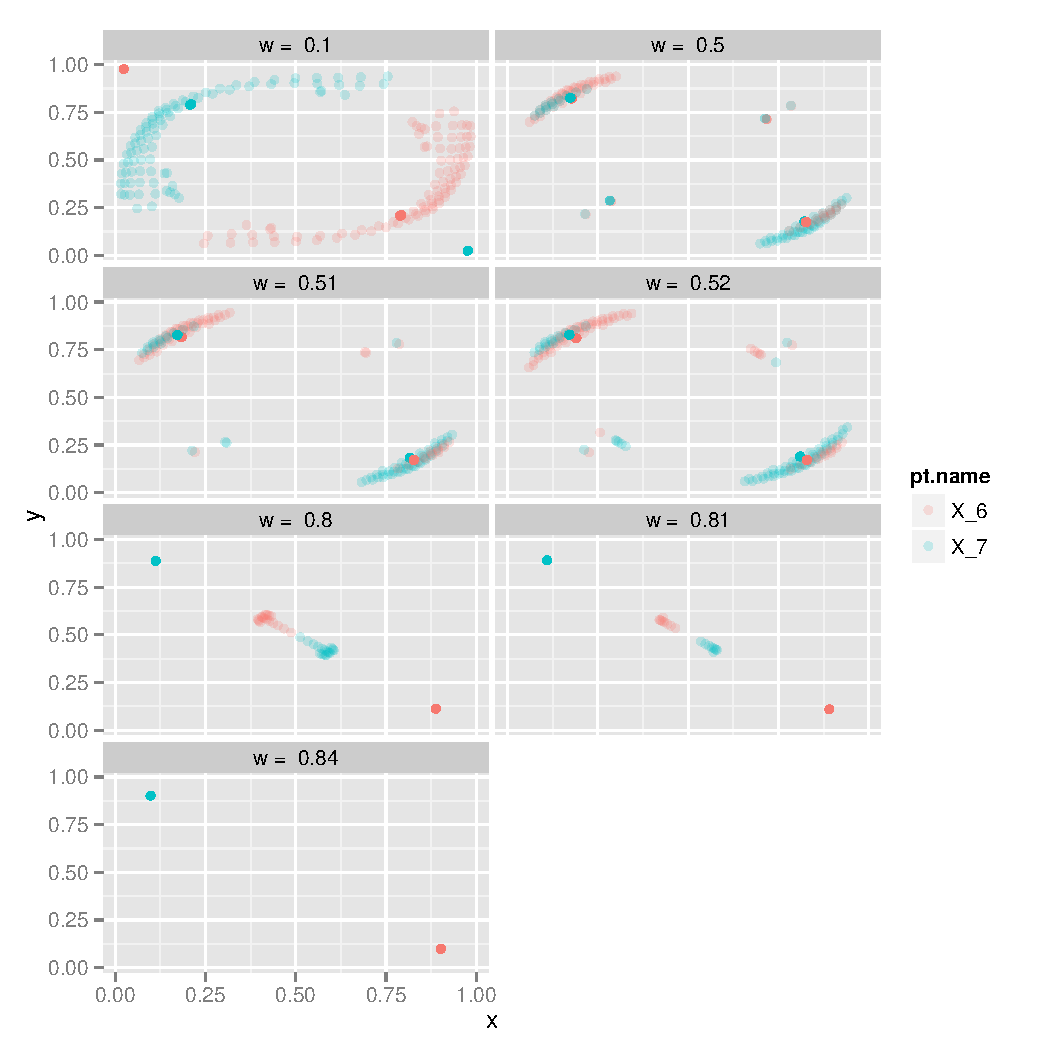
\includegraphics[width=\maxwidth]{figure/plot_final_pts} 

\end{knitrout}


\begin{knitrout}
\definecolor{shadecolor}{rgb}{0.969, 0.969, 0.969}\color{fgcolor}\begin{kframe}
\begin{alltt}
\hlkwa{for} \hlstd{(w.it} \hlkwa{in} \hlstd{w.vals) \{}
    \hlstd{sub.final.pts.lf.logical} \hlkwb{<-} \hlstd{all.final.pts.lf}\hlopt{$}\hlstd{w} \hlopt \hlstd{w.it}
    \hlstd{sub.final.pts.lf} \hlkwb{<-} \hlstd{all.final.pts.lf[sub.final.pts.lf.logical, ]}
    \hlkwd{levels}\hlstd{(sub.final.pts.lf}\hlopt{$}\hlstd{w)} \hlkwb{<-} \hlkwd{paste}\hlstd{(}\hlstr{"w="}\hlstd{,} \hlkwd{levels}\hlstd{(sub.final.pts.lf}\hlopt{$}\hlstd{w))}
    \hlstd{g1} \hlkwb{<-} \hlkwd{ggplot}\hlstd{(sub.final.pts.lf,} \hlkwd{aes}\hlstd{(}\hlkwc{x} \hlstd{= x,} \hlkwc{y} \hlstd{= y,} \hlkwc{colour} \hlstd{= pt.name))} \hlopt{+} \hlkwd{geom_point}\hlstd{(}\hlkwc{alpha} \hlstd{=} \hlnum{1}\hlopt{/}\hlnum{5}\hlstd{)} \hlopt{+}
        \hlkwd{scale_shape}\hlstd{(}\hlkwc{solid} \hlstd{=} \hlnum{FALSE}\hlstd{)}
    \hlstd{g1}
\hlstd{\}}
\end{alltt}
\end{kframe}
\end{knitrout}




\begin{figure}
\begin{minipage}[b]{0.5\linewidth}
\centering
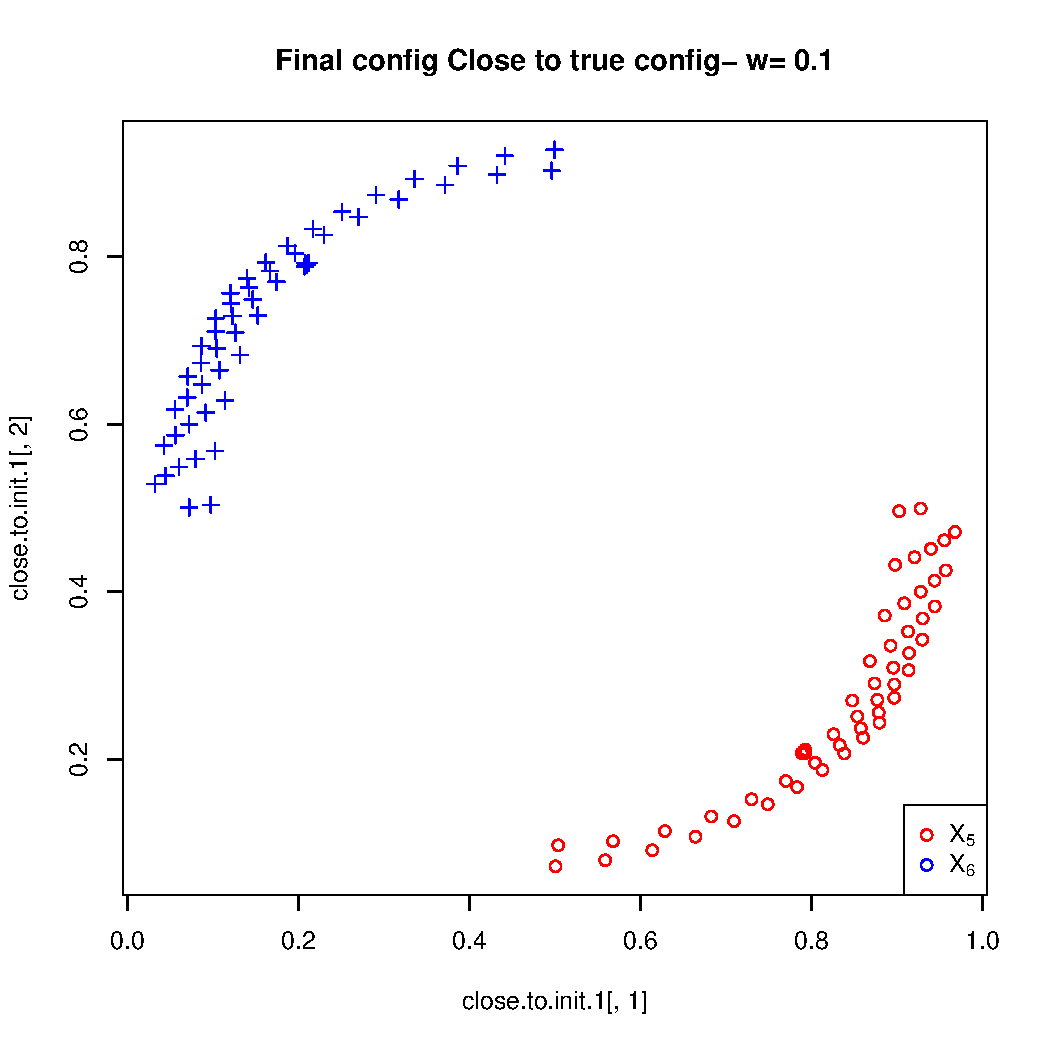
\includegraphics[scale=0.45]{true-min-w-0_1.pdf}

\label{fig:Finalconfig-MultMin-w-0_1_a}
\end{minipage}
\hspace{0.5cm}
\begin{minipage}[b]{0.5\linewidth}
\centering
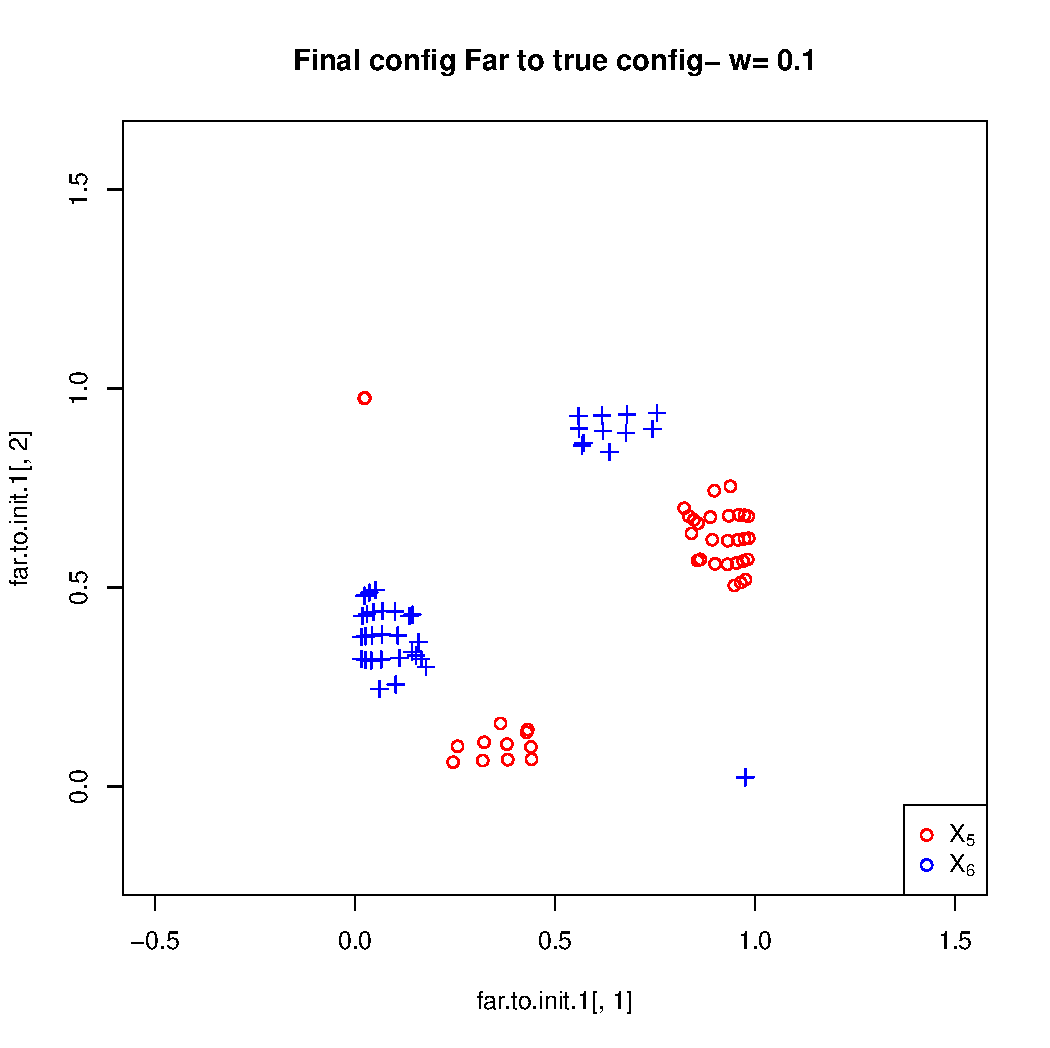
\includegraphics[scale=0.45]{other-min-w-0_1.pdf}

\label{fig:Finalconfig-MultMin-w-0_1_b}
\end{minipage}

\caption{Final configurations for for different $w=0.1$ }
\label{fig:Finalconfig-MultMin-w-0_1}


\end{figure}




\begin{figure}
\begin{minipage}[b]{0.5\linewidth}
\centering
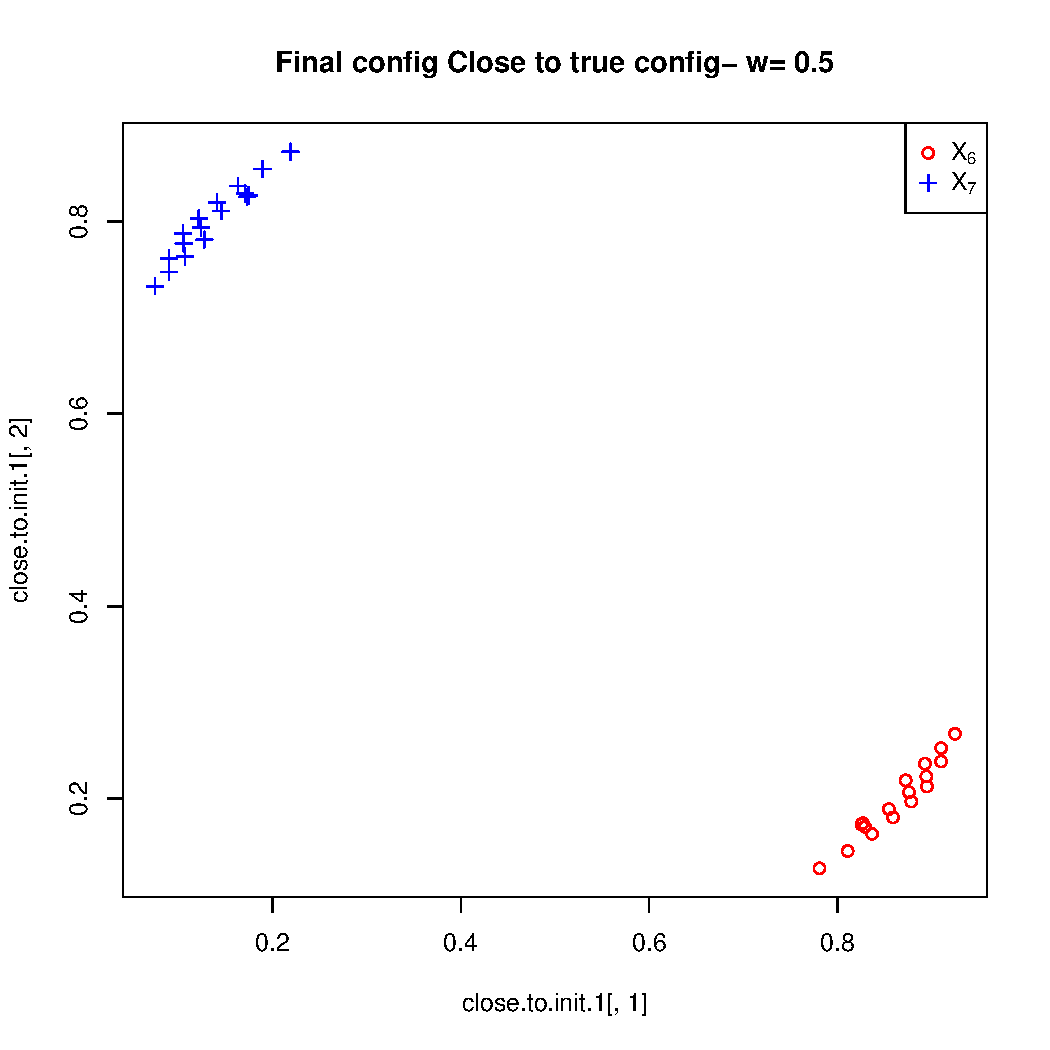
\includegraphics[scale=0.45]{true-min-w0_5}

\label{fig:Finalconfig-MultMin-w-0_5_a}

\end{minipage}
\hspace{0.5cm}
\begin{minipage}[b]{0.5\linewidth}
\centering
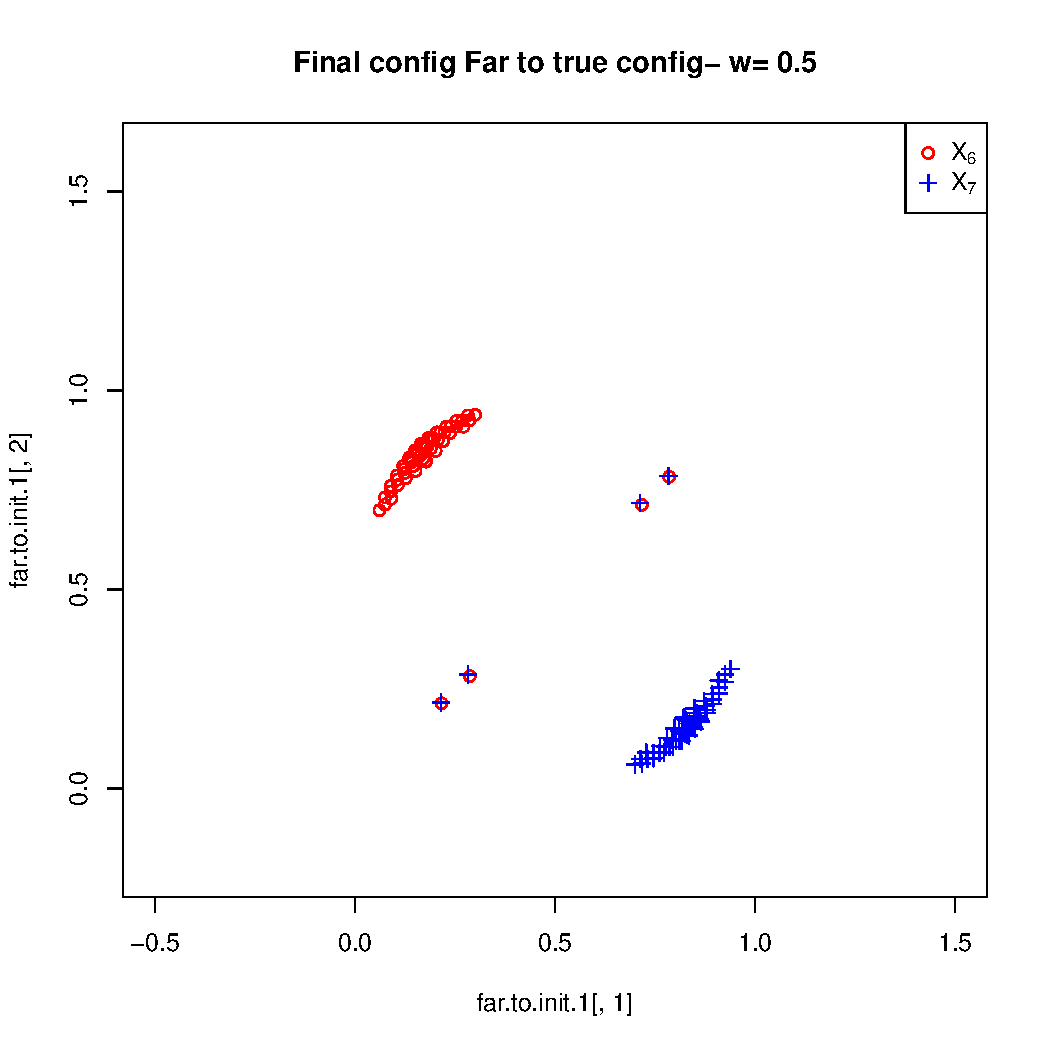
\includegraphics[scale=0.45]{other-min-w0_5.pdf}

\label{fig:Finalconfig-MultMin-w-0_5_b}

\end{minipage}

\caption{Final configurations for for different $w=0.5$ }
\label{fig:Finalconfig-MultMin-w-0_5}

\end{figure}

\begin{figure}
\begin{minipage}[b]{0.5\linewidth}
\centering
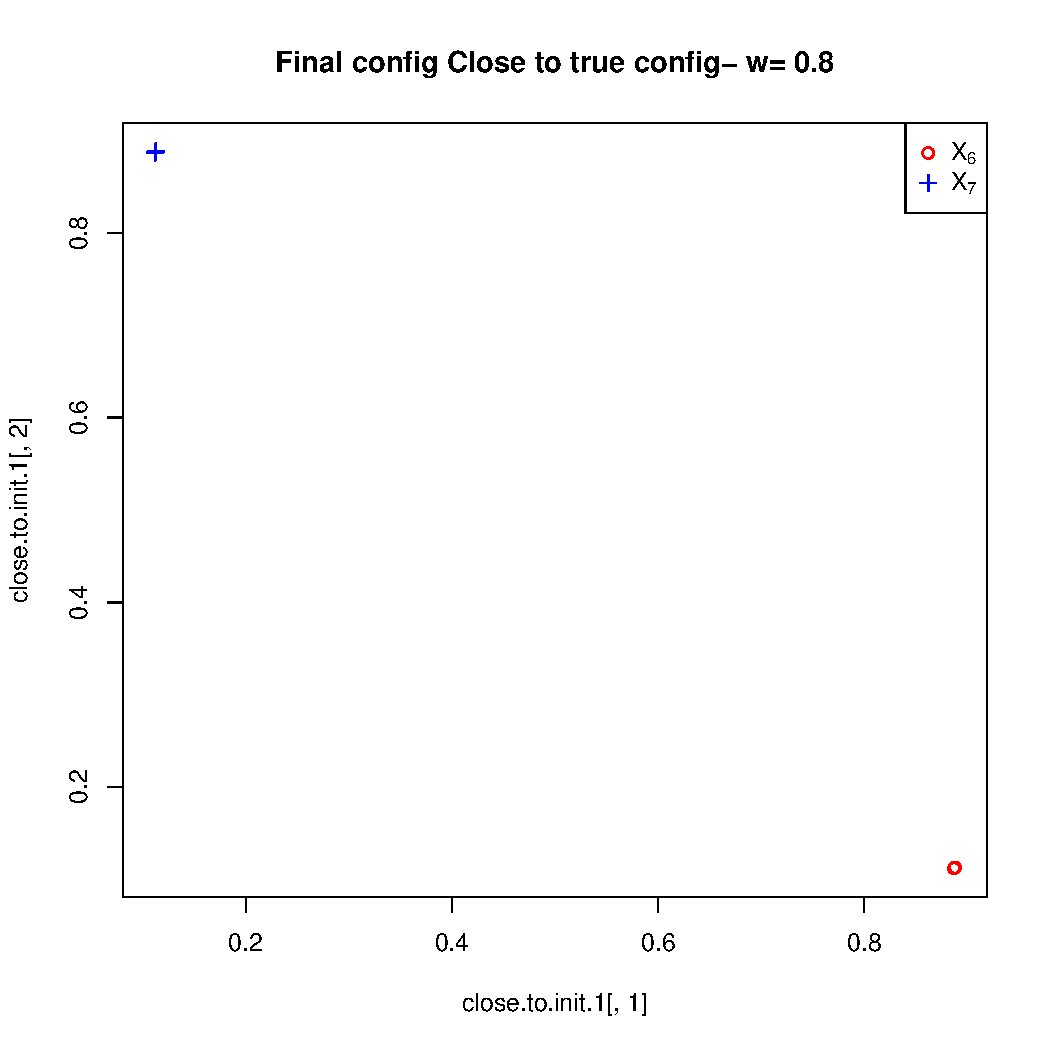
\includegraphics[scale=0.45]{true-min-w0_8.pdf}
\label{fig:Finalconfig-MultMin-w-0_8_a}


\end{minipage}
\hspace{0.5cm}
\begin{minipage}[b]{0.5\linewidth}
\centering
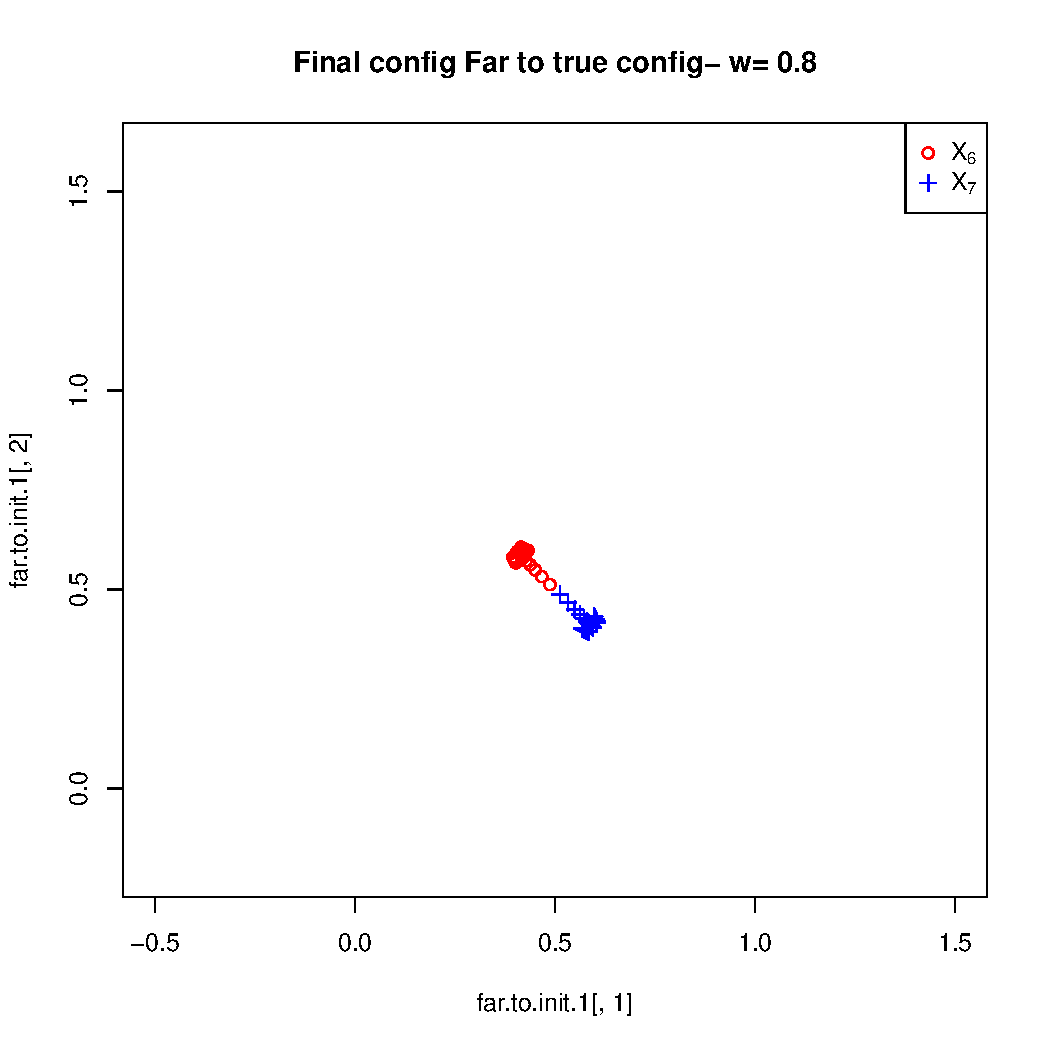
\includegraphics[scale=0.45]{other-min-w0_8.pdf}
\label{fig:Finalconfig-MultMin-w-0_8_a}


\end{minipage}

\caption{Final configurations for for different $w=0.8$ }
\label{fig:Finalconfig-MultMin-w-0_8}

\end{figure}



\begin{figure}
\begin{minipage}[b]{0.5\linewidth}
\centering
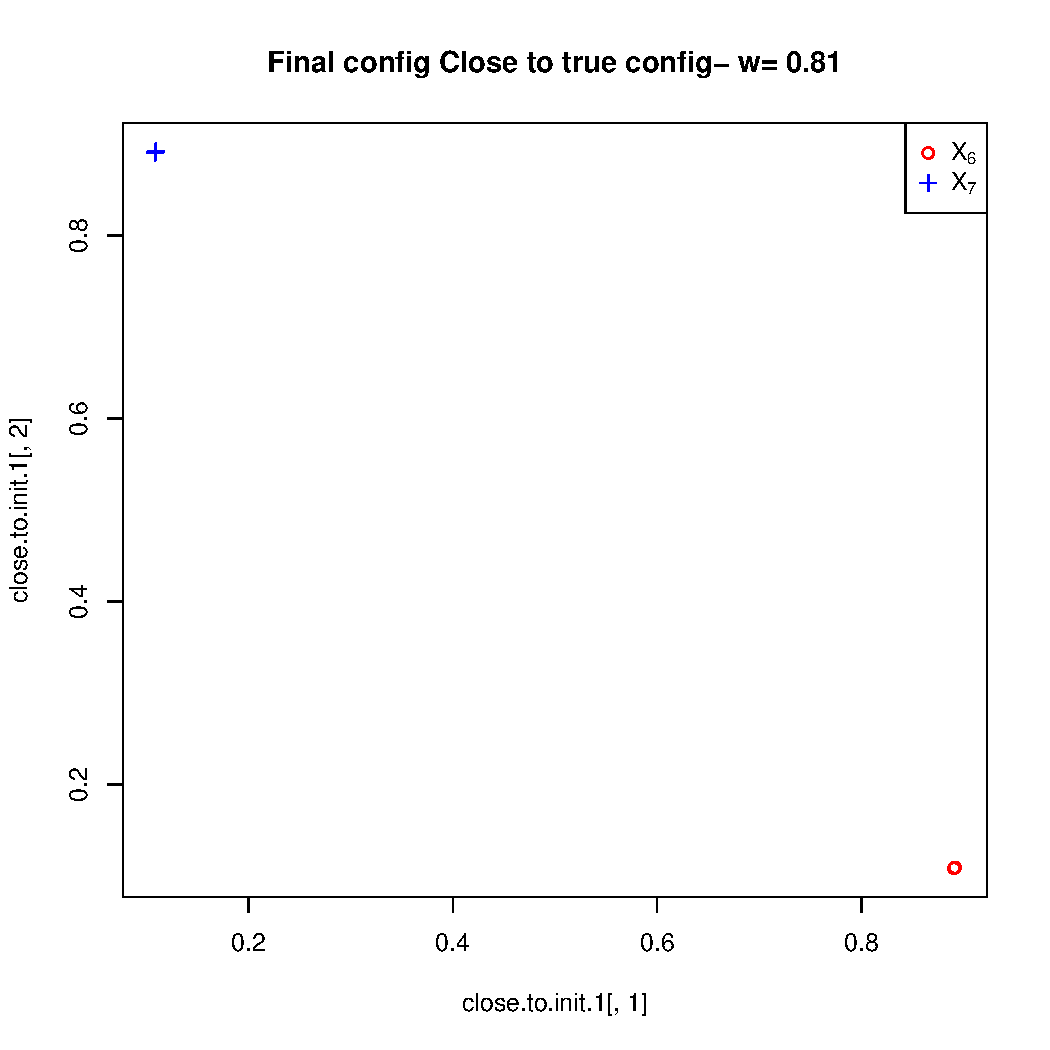
\includegraphics[scale=0.45]{true-min-w0_81.pdf}


\end{minipage}
\hspace{0.5cm}
\begin{minipage}[b]{0.5\linewidth}
\centering
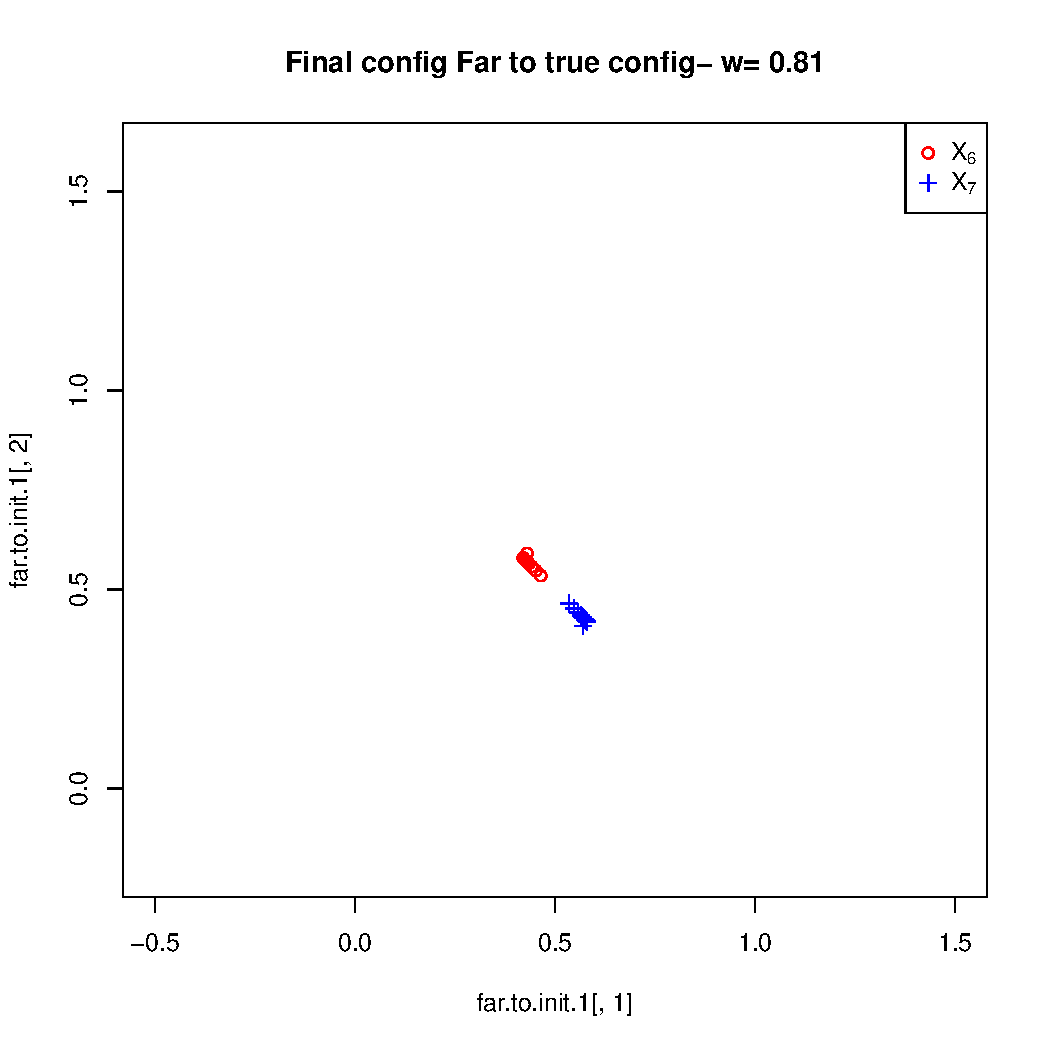
\includegraphics[scale=0.45]{other-min-w0_81.pdf}


\end{minipage}

\caption{Final configurations for for different $w=0.81$ }
\label{fig:Finalconfig-MultMin-w-0_81}

\end{figure}




\begin{figure}
\begin{minipage}[b]{0.5\linewidth}
\centering
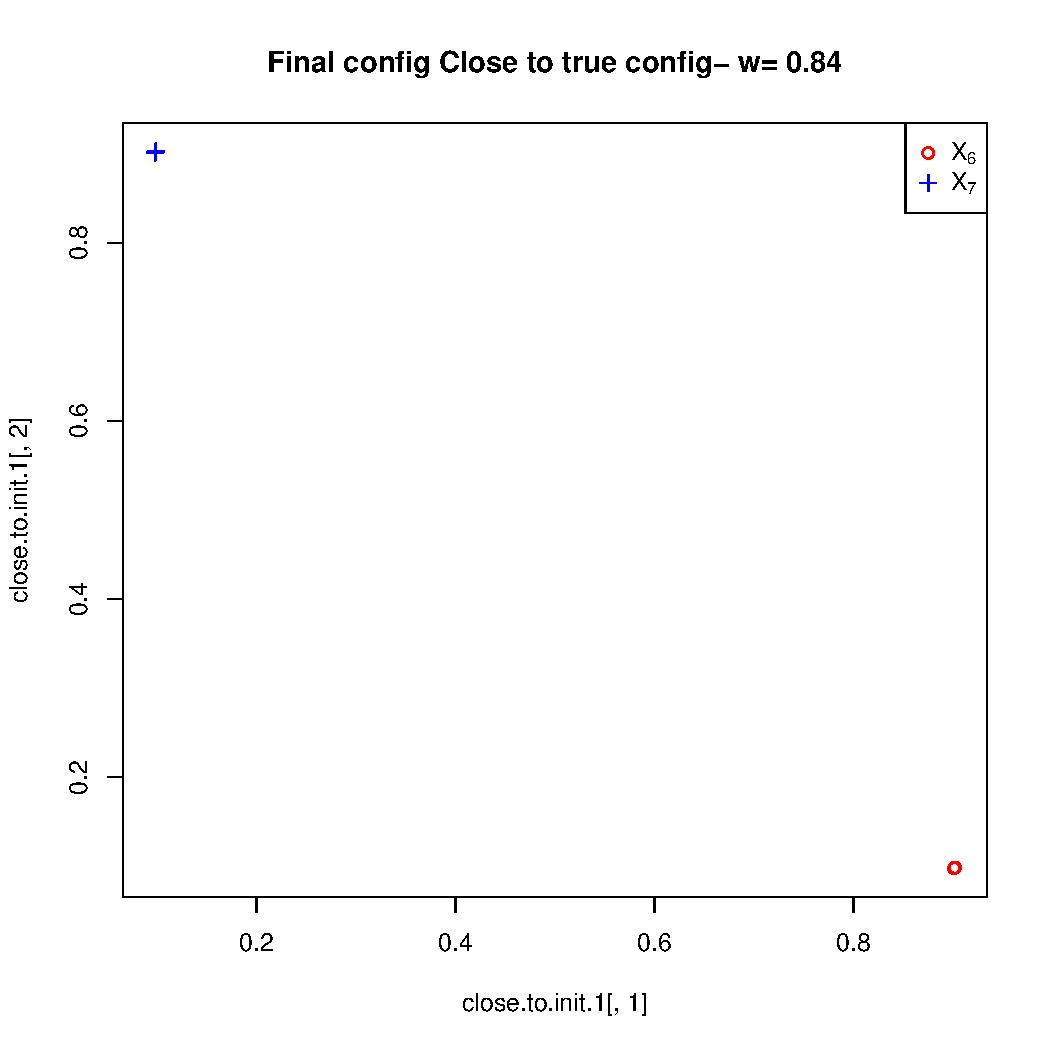
\includegraphics[scale=0.45]{true-min-w0_84.pdf}

\label{fig:figure2-1}
\end{minipage}
\hspace{0.5cm}
\begin{minipage}[b]{0.5\linewidth}
\centering
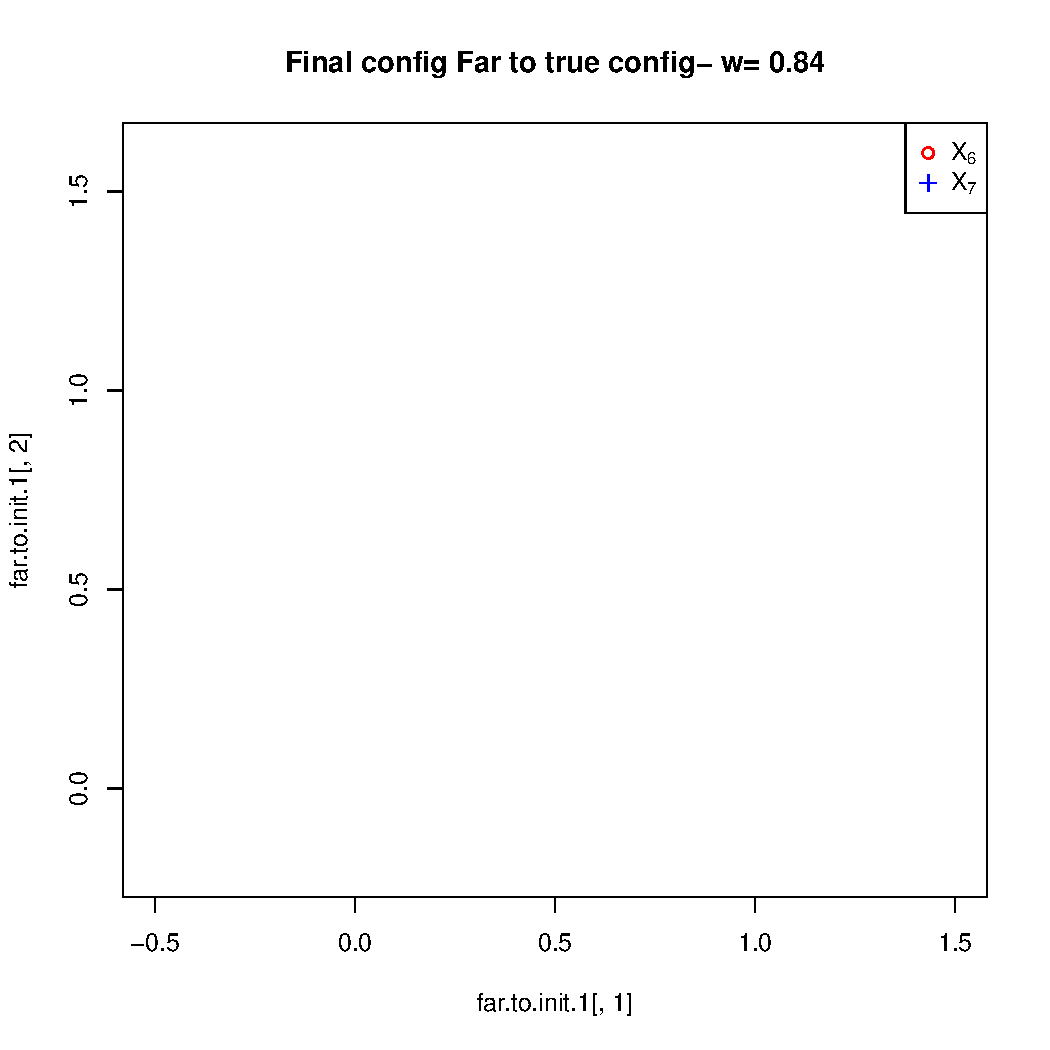
\includegraphics[scale=0.45]{other-min-w0_84.pdf}


\end{minipage}

\caption{Final configurations for for different $w=0.84$ }
\label{fig:Finalconfig-MultMin-w-0_84}

\end{figure}


% latex table generated in R 2.15.1 by xtable 1.7-0 package
% Sat Jan 05 00:54:38 2013
\begin{landscape}
\begin{table}[ht]
\def\h#1{\multicolumn{1}{p{3em}}{\mbox{}\hskip0pt #1}}
\begin{center}

\begin{tabular}{r|rrrrrrrrrrrrrrrrrrrrrrrrrrrrrrrrrrrr}
\hline
$w$ & 0.1 & 0.2 & 0.3 & 0.4 & 0.41 & 0.42 & 0.43 & 0.44 & 0.45 & 0.46 & 0.47  \\ 
\hline
Local min for real config. & 2.80 & 2.51 & 2.22 & 1.92 & 1.89 & 1.86 & 1.83 & 1.80 & 1.77 & 1.74 & 1.71 \\ 
Alternative local min & 0.39 & 0.76 & 1.10 & 1.40 & 1.43 & 1.46 & 1.48 & 1.51 & 1.53 & 1.56 & 1.58 \\ 
\hline
\end{tabular}


\begin{tabular}{r|rrrrrrrrrrrrrrrrrrrrrrrrrrrrrrrrrrrr}
\hline
$w$ & 0.48 & 0.49 & 0.5 & 0.51 & 0.52 & 0.53 & 0.54 & 0.55 & 0.6 & 0.65 & 0.7 \\ 
\hline
Local min for real config. &  1.68 & 1.65 & 1.62 & 1.59 & 1.56 & 1.53 & 1.50 & 1.47 & 1.32 & 1.17 & 1.01   \\ 
Alternative local min &  1.60 & 1.63 & 1.65 & 1.67 & 1.69 & 1.71 & 1.73 & 1.74 & 1.81 & 1.82 & 1.81  \\ 
\hline
\end{tabular}



\begin{tabular}{r|rrrrrrrrrrrrrrrrrrrrrrrrrrrrrrrrrrrr}
\hline
$w$ & 0.75 & 0.76 & 0.77 & 0.78 & 0.79 & 0.8 & 0.81 & 0.82 & 0.83 & 0.84 & 0.85  \\ 
\hline
Local min for real config. &  0.86 & 0.82 & 0.79 & 0.76 & 0.73 & 0.70 & 0.66 & 0.63 & 0.60 & 0.57 & 0.53  \\ 
Alternative local min &   1.79 & 1.77 & 1.75 & 1.72 & 1.69 & 1.66 & 1.64 & NA & NA & NA & NA \\ 
\hline
\end{tabular}

\end{center}

\label{stress-val-table}
\end{table}
\end{landscape}


\begin{comment}
%old results

\begin{table}[ht]
\begin{center}
\begin{tabular}{rrrrrr}
\hline
$w$ value & 0.1 & 0.45 & 0.5 & 0.55 & 0.99 \\ 
\hline
Local min for real config. & 2.80 & 1.77 & 1.62 & 1.47 & 0.04 \\ 
Alternative local min & 0.39 & 1.53 & 1.65 & 1.74 & NA \\ 
\hline
\end{tabular}
\end{center}
\label{stress-val-table}
\end{table}
\end{comment}

Other than such carefully constructed examples, it is  unexpected that slight changes in $w$  will change the ordering of the ``distinct''  local minima according to their stress values.
Therefore,  the argmin among the local minima configurations is independent of $w$. The minimum configuration is then a continuous function of $w$. 
By the continuity of the distance function with respect to configurations, the test statistic is continuous with respect to $w$. One can conclude  that stochastic continuity  is a valid assumption and $\beta(w) $ is a continuous function of $w$. 
%It is possible this is not the global minimum in $\mathbb{R}^d$  

%Does the discontinuity in configurations mean discontinuity  in the $\beta(w)$ function
%It is possible this is not the global minimum in $\mathbb{R}^d$  

\begin{comment}

\includegraphics{FidCommPaper-fig-stats-p}



, so any $w$ value that takes advantage of this situation and captures fidelity will limit the growth of the test statistic under alternative. So such $w$ values that are small enough to preserve fidelity, yet large enough to not lose significantly from commensurability will have increases in power to become $w^*$. 




Consider  an increase in $r$, this will cause the test statistic under null to be stochastically smaller,
leading to a smaller critical value. So , a increase in priority of fidelity,
which corresponds to smaller $w$ might lead to the increase in the test statistic under alternative, and therefore an increase in power.\ref{fig-stats-r}  



\includegraphics{FidCommPaper-fig-stats-r}

Consider increases in $c$, which will increase the dissimilarity  both between matched and between unmatched vectors. 



\includegraphics{FidCommPaper-fig-stats-c}




Consider increases in $q$,  the test statistic under both null and alternative is inflated\ref{fig-stats-q}. 


\includegraphics{FidCommPaper-fig-stats-q}
If commensurability can be preserved in the face of the increase in $q$, the power of the test may be preserved. However a very large increase in $w$ is not guarenteed to increase the preservation of commensurability, since the extra dimensions are noise, trying to   make the differences between coordinates  small in those dimensions will not  help in power, in fact may be disruptive since,
more fidelity may be lost in the effort to bring the pair of points together.

\end{comment}


%\section[Optional table of contents heading]{Dependence of globality of local minima on $w$}




\chapter{Simulations and Experiments}
\label{sec:simexp_results}
\chaptermark{Simulations and Experiments}


\section{Two data settings for Match Detection}


  Before introducing the match detection task, two data models are proposed that illustrate the idea of matchedness.
\subsection{Gaussian setting\label{subsec:GaussianSet}}
  Let    $\Xi_1 = \mathbb{R}^{p}$ and $\Xi_2 = \mathbb{R}^{p}$.
  Let $\bm{\alpha}_i \sim^{iid} MVNormal(\bm{0},I_p)$ represent $n$ ``objects".  Let $X_{ik} \sim^{iid} MVNormal(\bm{\alpha_i},\Sigma)$ represent $K=2$ matched measurements (each under a different condition).
  $\Sigma$ is a positive-definite $p\times p$ matrix such that  $\max(\Lambda(\Sigma))=\frac{1}{r} $ where $\Sigma=U\Lambda(\Sigma)U'$  is the eigenvalue decomposition of $\Sigma$. See Figure~\ref{fig:Fig1}.

The parameter $r$ controls the variability between ``matched" measurements. If $r$ is large, it is expected that the distance between matched measurements
$X_{i1}$ and $X_{i2}$ to be stochastically smaller than $X_{i1}$ and $X_{i'2}$ for $i \neq i'$ ; if r is small, then ``matched" is not informative in terms of similarity of measurements.
 Smaller $r$ will make the decision problem harder and will lead to higher rate of errors or tests with smaller power for fixed type I error rate $\alpha$.
  
    \begin{figure}
	\begin{center}
    \includegraphics[scale=0.75]{MVN_alpha_r_multiple_sancar.pdf}
    \caption{For the  Gaussian setting (Section \ref{subsec:GaussianSet}), the $\alpha_i$ are denoted by black points and the $X_{ik}$ are denoted by red and blue points respectively.}
\label{fig:Fig1}
	\end{center}
  \end{figure}

\subsection{Dirichlet setting\label{subsec:DirichletSet}}
Let $S^p=\{\bm{x}:\bm{x}\in\mathbb{R}^{(p+1)}, \sum_{l=1}^p{x_l}=1\}$ be the standard $p$-simplex in $\mathbb{R}^{p+1}$.
 Let $\Xi_1 = S^p$ and $\Xi_2 = S^p$.   Denote a vector of ones by $\bm{1}_{p+1}\in \mathbb{R}^{(p+1)}$.
  Let $\bm{\alpha}_i \sim^{iid} Dirichlet(\bm{1}_{p+1})$ represent $n$  ``objects'' and let $X_{ik} \sim^{iid} Dirichlet(r\bm{\alpha}_i+\bm{1}_{p+1})$ represent $K$ measurements. See Figure~\ref{fig:Fig2}.

 The parameter $r$ again controls the variability between ``matched" measurements.
    \begin{figure}
	\begin{center}
    \includegraphics[scale=0.75]{Dirichlet_alpha_r_multiple_sancar.pdf}
   \caption{ For the  Dirichlet setting (Section \ref{subsec:DirichletSet}),  the $\alpha_i$ are denoted by black points and the $X_{ik}$ are denoted by red and blue points respectively.}
\label{fig:Fig2}
	\end{center}
  \end{figure}

\subsection{Noise\label{noise}}
Measurements $X_{ik}$ carry the signal that is relevant to the exploitation task. Noise dimensions can be introduced to  the measurements by concatenating a $q$-dimensional error vector whose magnitude is controlled by the parameter $c$. The noisy measurements will be  represented by the random vectors 
 \begin{equation}
\breve{X}_{ik}=[(1-c)X_{ik}\hspace{5pt} cE_{ik}]\label{eq:noise-expr}
\end{equation}
 where $E_{ik} \sim^{iid} Dirichlet(\bm{1}_{(q+1)})\label{eq:noise-model-dir} $ for the Dirichlet setting and $E_{ik} \sim^{iid} MVNormal(\bm{0} , (1+\frac{1}{r})I_{q+1}) \label{eq:noise-model-mvn} $ for the Gaussian setting. $\breve{X}_{ik}$ will be used instead of ${X}_{ik}$ for computing dissimilarities in the ``noisy" version of the problem. These noisy measurements allow the comparison of  different methods applied to the problem with respect to their robustness.
  





%Let us first investigate the effect of parameters on the empirical distribution of the test statistic, under null and alternative.
% For our Multivariate Normal and Dirichlet models, consider the signal and noise dimensions $p$ and $q$ respectively.
%  An increase in $p$ leads to the inflation of the test statistic under alternative
%  \ref{fig-stats-p}.


\section{Simulation Results\label{sec:Simulation Results}}
To compare the  different approaches, training data of matched sets of measurements were generated according to the Dirichlet and Gaussian settings. Dissimilarity representations were computed from pairwise Euclidean distances of these measurements. A set of matched pairs and unmatched pairs of measurements were also generated for testing with the same distributions. Following the out-of-sample embedding of the dissimilarities test pairs (computed via by one of the three P$\circ $M, CCA and JOFC approaches)  test statistics  for matched and unmatched pairs were used to compute power values at a set of fixed type I error rate $\alpha$ values.

 Additionally, to take robustness of methods into consideration, ``noisy" measurements were created from the original measurements by concatenating randomly generated independent noise vectors (subsection \ref{noise}).   This setting will be referred to as the ``noisy case". The magnitude of noise is controlled by the parameter $c$ in equation \eqref{eq:noise-expr}). The original setting, with $c=0$,  will be referred as the ``noiseless case".
If the magnitude of noise is small enough, and the embedding dimension is not larger than signal dimension, the embeddings provided by PCA and MDS will not be affected significantly. However  if the number of noisy dimensions (controlled by the parameter $q$ in the distribution of $E_{ik}$ as defined in equation \eqref{eq:noise-expr}) is large enough, embeddings via  CCA  will be affected due to spurious correlation between noisy dimensions.

Given the setting ("Gaussian","Dirichlet"),   the steps for each Monte Carlo replicate are as follows:
\begin{itemize}
\item A training set ($\mathbf{T}_{mc}$) which consists of  $n$ pairs of matched measurements is generated.  If $c=0$, the ``noiseless" data setting is being simulated and measurements are $p$-dimensional vectors, otherwise  the ``noisy" setting is being used to generate data and measurement vectors are $(p+q)$-dimensional. $ \mathbf{T}_{mc}$ = 
$\begin{array}{ccc}
        X_{11} & \ldots & X_{1K} \\
        \cdots & \cdots      & \cdots   \\ 
        X_{n1} & \ldots     & X_{nK} \\
    \end{array}
$
 where each $X_{ik}$ is a random vector of dimension $(p+q \times I(c>0))$ and the conditional distribution  $X_{i.}|\bm{\alpha}_i  $ is specified as an appropriate Multivariate Normal or Dirichlet distribution.
\item Dissimilarities are computed and embedded in  Euclidean space  via MDS (followed by a transformation from  $\mathbf{R}^d$ to  $\mathbf{R}^d$ and  projection into $\mathbf{R}^d$, respectively  for P$\circ$M and CCA) . The final embeddings lie in $\mathbb{R}^d$.   Denote this in-sample embedding configuration as   $\hat{\mathbf{T}}$. Note that  if the JOFC method is being used, embedding is carried out with the weighted raw stress function $\sigma_{W}(\cdot)=f_{w}(D(\cdot),M)$ in equation \eqref{fid-comm-tradeoff-func} with a common weight $w$ for commensurability terms and another common weight $1-w$ for fidelity terms, otherwise unweighted raw stress function ($\sigma(\cdot)$) is used as a criterion function for embedding.

\item  $m$ pairs of matched   measurements are generated which are treated as out-of-sample, and 
\begin{itemize}
\item compute the dissimilarities  %$\mathbf{\Delta}^{new}={ \delta_{ik}^{new}; i=1,\ldots, n;\hspace{5pt} k=1,2}$
 between these out-of-sample  points and the points in ${\mathbf{T}_{mc}}$,  
\item  embed the OOS dissimilarities as pairs of embedded points via the OOS extension:\\
 $(\tilde{y}_1^{(1)},\tilde{y}_1^{(2)}),\ldots, (\tilde{y}_m^{(1)},\tilde{y}_m^{(2)})$, 
\item compute the test statistic $\tau$ for each pair.%, $t(\tilde{y}_i^{(1)},\tilde{y}_i^{(2)});\hspace{4pt}
%i=1,\ldots,m$
\end{itemize}
 The values of the statistic $\tau$ are used for computing  the empirical cumulative distribution function under null hypothesis. 

\item Identical steps for $m$ pairs of unmatched measurements result in the empirical cumulative distribution  function of $\tau$ under alternative hypothesis.
\item For any fixed $\alpha$ value, a critical value for the test statistic and the corresponding power is computed.
\end{itemize}



\begin{figure}
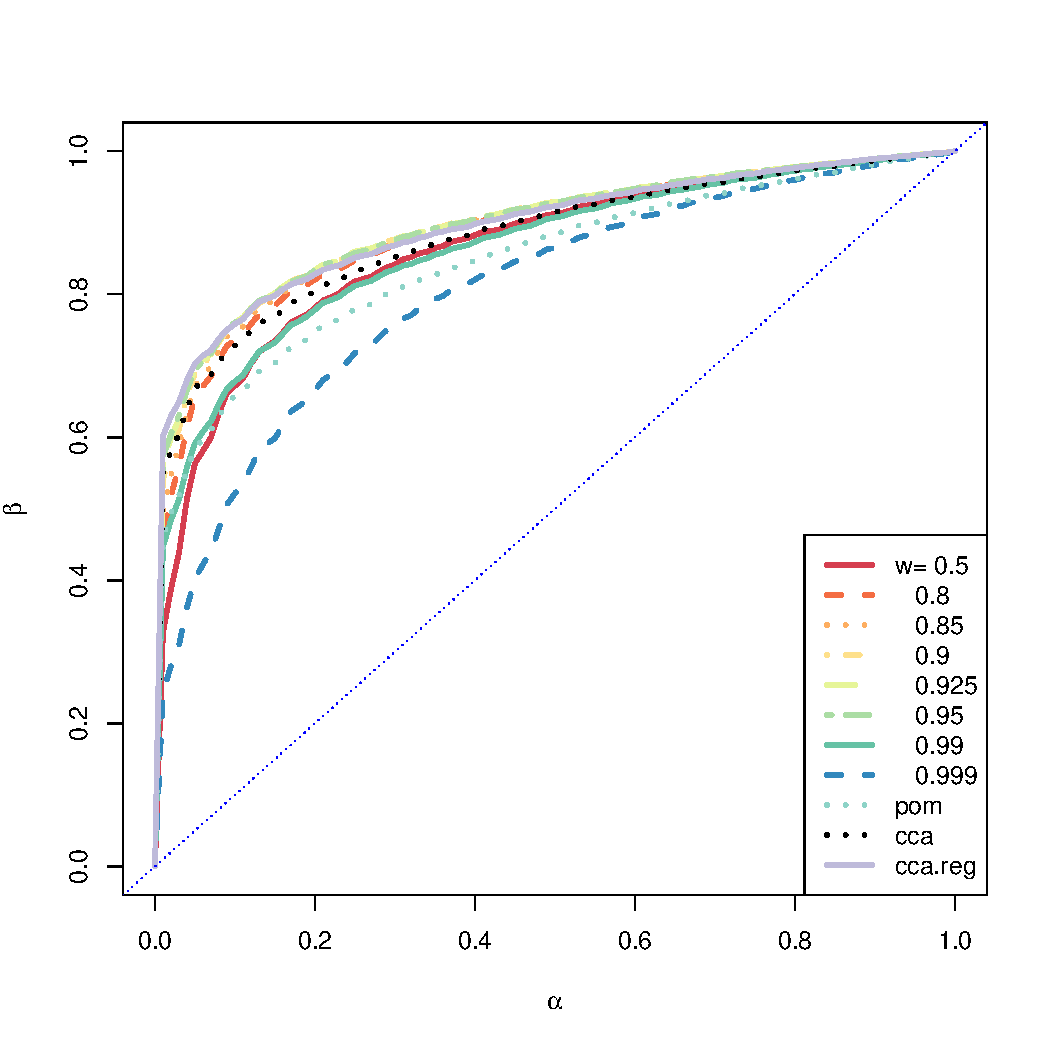
\includegraphics[scale=0.75]{MVN-FC-Tradeoff-OOS-c0_01.pdf}
\caption{Power ($\beta$) vs Type I error ($\alpha$) plot for different $w$ values for the Gaussian setting (noisy case)}
\label{fig:MVN-c001-power-alpha}
\end{figure}

\begin{figure}
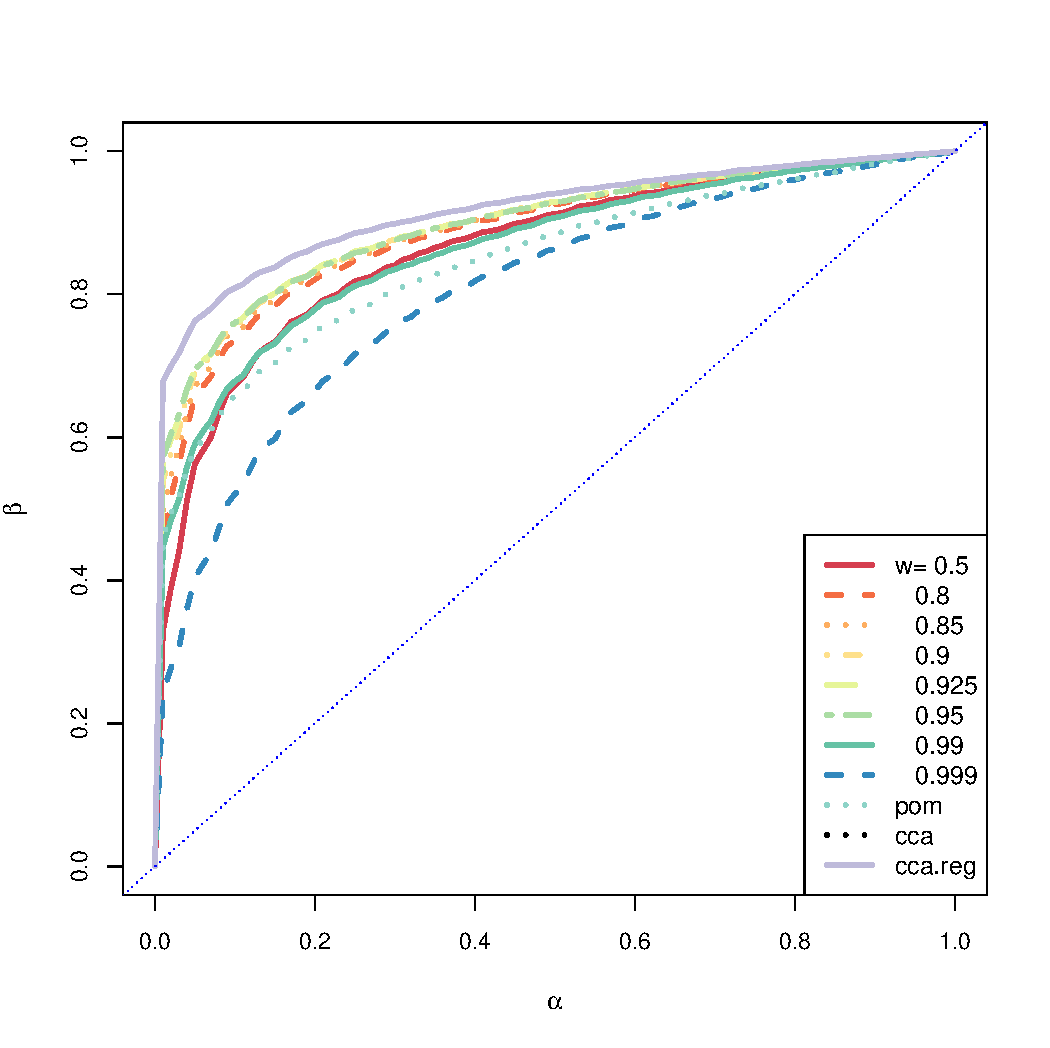
\includegraphics[scale=0.75]{MVN-FC-Tradeoff-OOS-c0.pdf}
\caption{Power ($\beta$) vs Type I error ($\alpha$) plot for different $w$ values for the Gaussian setting (noiseless case)}
\label{fig:MVN-c0-power-alpha}
\end{figure}

\begin{figure}
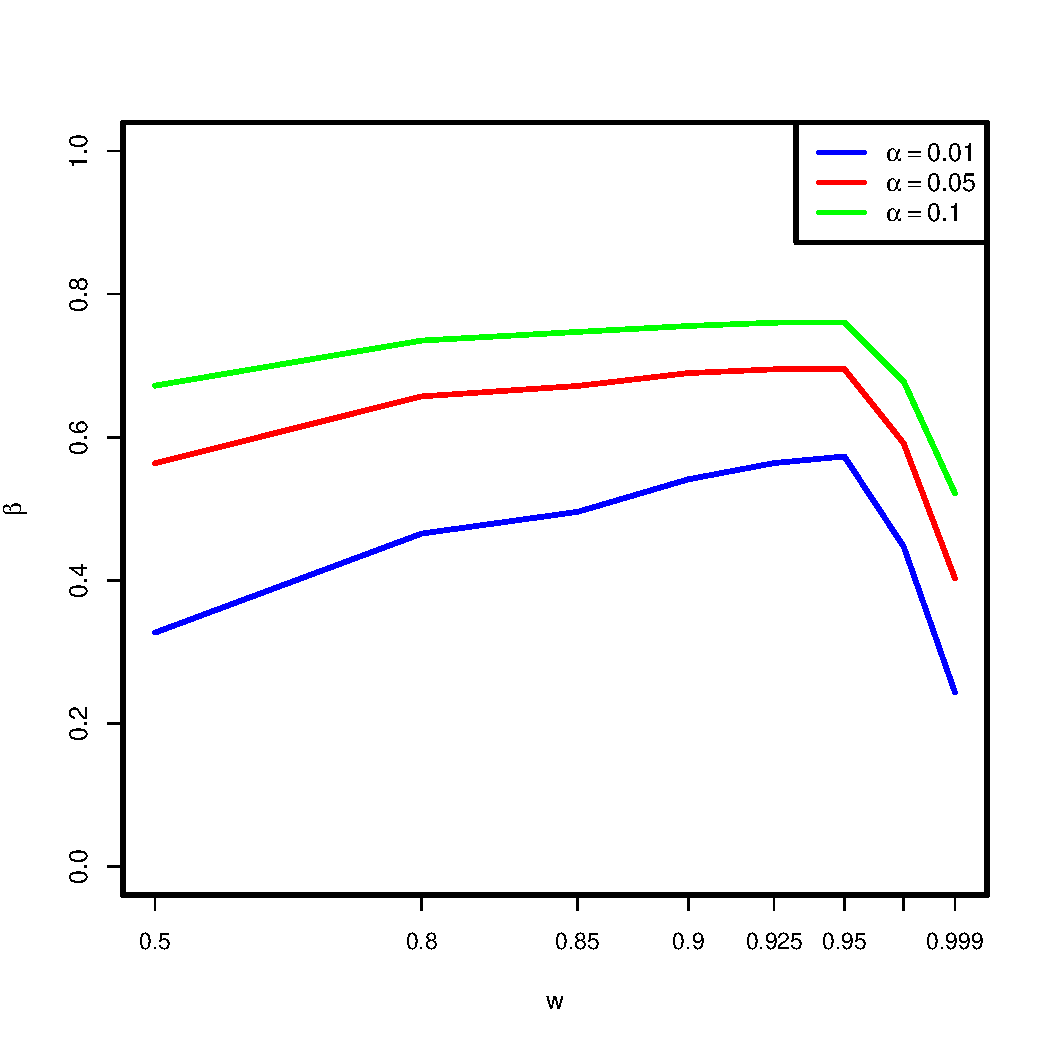
\includegraphics[scale=0.95]{OOSMVN-power-w-c0_01.pdf}
\caption{Power ($\beta$) vs $w$ plot for different Type I error ($\alpha$) values for the Gaussian setting (noisy case)}
\label{fig:MVN-c001-power-w}
\end{figure}


\begin{figure}
\includegraphics[scale=0.75]{Dirichlet-FC-Tradeoff-OOSc0-01-n150.pdf}
\caption{Power ($\beta$) vs Type I error ($\alpha$) plot for different $w$ values for the Dirichlet setting (noisy case)}
\label{fig:Dir-c001-power-alpha}
\end{figure}

\begin{figure}
\includegraphics[scale=0.75]{Dirichlet-FC-Tradeoff-OOSc0-n150.pdf}
\caption{Power ($\beta$) vs Type I error ($\alpha$) plot for different $w$ values for the Dirichlet setting (noiseless case)}
\label{fig:Dir-c0-power-alpha}
\end{figure}

\begin{figure}
\includegraphics[scale=0.95]{OOSDirichlet-power-w-c0-01.pdf}
\caption{Power ($\beta$) vs $w$ plot for different Type I error ($\alpha$) values for the Gaussian setting (noisy case)}
\label{fig:Dir-c001-power-w}
\end{figure}

Setting p and q to 5 and 10, respectively, for $n=150$ and $m=150$, the average of the power values for $nmc=150$ Monte Carlo replicates are computed at  different $\alpha$s and are plotted in Figure \ref{fig:MVN-c001-power-w} against $\alpha$ for the Gaussian setting.  Qualititatively similar plots for the Dirichlet setting  are not included for brevity.  The plot in Figure \ref{fig:MVN-c001-power-w} shows that for different values of  $w$, $\beta$-$\alpha$ curves vary significantly.  The conclusion is that the match detection tests with JOFC embedding using specific $w$ values have better performance than other $w$ values in terms of power.  In Figure
 \ref{fig:MVN-c001-power-w},  $\beta(w)$ is plotted against $w$ for fixed values of $\alpha$. It is  interesting that the optimal value of $w$ seems to be in the range of $(0.85,1)$ for all settings, which suggests a significant emphasis on commensurability might be  critical for the match detection  task. 




\begin{comment}
\begin{figure}
\includegraphics[scale=0.75]{OOS-MVN-power-w-c0.pdf}
\caption{$\beta$ vs $w$ plot for fixed $\alpha$ values for the Gaussian setting (noiseless case)}
\label{fig:MVN-c0-beta-w}
\end{figure}


\begin{figure}
\includegraphics[scale=0.65]{OOSMVN-power-w-c001.pdf}
\caption{Power ($\beta$) vs $w$ plot for fixed Type I error ($\alpha$) values for the Gaussian setting (noisy case)}
\label{fig:MVN-c001-beta-w}
\end{figure}

\end{comment}

Note that in Figure \ref{fig:MVN-c001-power-w} for $\alpha=0.05$, $\beta_{\alpha=0.05}(w=0.99)\geq\beta_{\alpha=0.05}(w=0.5)$. However, for $\alpha=0.3$, $\beta_{\alpha=0.3}(w=0.99)\leq\beta_{\alpha=0.3}(w=0.5)$. This justifies our comment that  $w^{*}$  must be defined with respect to  the AUC measure or a specific $\alpha$ value.


\begin{comment}
\begin{figure}
\includegraphics[scale=0.75]{OOS-Dirichlet-power-w-c0.pdf}
\caption{$\beta$ vs $w$ plot for fixed $\alpha$ values for the Dirichlet setting(noiseless case)}
\label{fig:fig7}
\end{figure}

\begin{figure}
\includegraphics[scale=0.35]{OOS-Dirichlet-power-w-c0-01.pdf}
\caption{$\beta$ vs $w$ plot for fixed $\alpha$ values for the Dirichlet setting(noisy case)}
\label{fig:fig8}
\end{figure}
\end{comment}



Note that  for all of the settings, the estimate of the optimal $w^{*}$ has  higher power than $w$=0.5 (the unweighted case).
To test the statistical significance of this observation,   the null hypothesis that  $H_{0}: \beta_{\alpha}({\hat{w}^*})\leq\beta_{\alpha}({w=0.5})$  is tested against the alternative $H_{A}=\beta_{\alpha}({\hat{w}^*})>\beta_{\alpha}({w=0.5})$.  The least favorable null hypothesis is that  $H_{0}: \beta_{\alpha}({\hat{w}^*})=\beta_{\alpha}({w=0.5})$.
Using previous notation,  the test statistic will be denoted by $T_a(w)$ under the alternative hypothesis and $T_0(w)$ under the null hypothesis.

McNemar's test will be used to compare the two predictors (referred to as $C_1$ and $C_2$ with $w$=0.5 and $w$=$w^*$ at a fixed $\alpha$ value.

For a fixed $\alpha$ value, one can compute two critical values $c(0.5)=max_l \{  P(T_0(0.5)>c)<\alpha\}$,  $c(w^*)=max_l \{  P(T_0(w_2)>c)<\alpha\}$. The values of the decision function that uses these critical  values, for each pair of embedded points (indexed by $i$, are  $(\tilde{y}_i^{(1)},\tilde{y}_i^{(2)}),\hspace{7pt}i=1,\ldots,m$. To compare the  two statistical tests with  $w=0.5$ and $w$=$w^*$  , one can prepare a $2\times 2$ contingency-table of correct decisions and incorrect decisions made by each statistical test (or equivalently true and false classifications made by two classifiers). Denote decision outcome as $g_1$ for the first statistical test and $g_2$ for the second statistical test. If $g_1=True$ and $g_2=False$ for an instance,  the first test made the correct decision and the second test made the incorrect decision with regard to the null and alternative hypotheses.
% McNemar's test was used to compare the two contingency tables for fixed $\alpha$. McNemar's test is a statistical test for %comparing two binary classifiers based on a 2-by-2 table of the counts of misclassifications of each. That is,
Consider the contingency table for a Monte Carlo replicate given by $$G^{(l)}= \begin{array}{|c|c|}
      \hline
       e_{FF}^{(l)} & e_{TF}^{(l)}\\
      \hline
       e_{FT}^{(l)} & e_{TT}^{(l)}\\
      \hline
      \end{array}      $$  where $l$ is the index of the MC replicate, $e_{g_1g_2}^{(l)}$ is equal to the number of instances at which the true hypothesis were identified  correctly ($g_1=True$) or incorrectly ($g_1=False$) by the first test, and correctly ($g_2=True$) or incorrectly ($g_2=False$) by the second test in that MC replicate.

Under the null  hypothesis that the two predictors have the same power at $\alpha$ ,
 $Pr[\left(g_1g_2\right)=(TF)]=Pr[\left(g_1g_2\right)=(FT)]$, so $\sum_l{I \{e_{TF}^{(l)}>e_{FT}^{(l)}\}}$ will be distributed according to  the binomial distribution, $\mathcal{B}(nmc,0.5)$. ($I\{\cdot\}$ is the indicator function.) 

% For each Monte Carlo replicate, the p-value of McNemar's test was computed separately.

\begin{comment}
\begin{figure}
\begin{tabular}{p{4.7cm}p{4.7cm}}
$e_{00}$:Misclassified by \newline Both $C_1$ and $C_2$ & $e_{10}$:Correctly Classified by $C_1$,\newline Misclassified by $C_2$\\
& \\
$e_{01}$:Correctly Classified by $C_1$, \newline Misclassified by $C_2$ & $e_{11}$:Correctly Classified by \newline Both $C_1$ and $C_2$
\end{tabular}. 

\caption{Contingency Table for McNemar's test for comparing two classifiers, $C_1$ and $C_2$}
\label{fig:cont-table}
\end{figure}
\end{comment}

For the noisy version of the Gaussian setting at allowable type I error 0.05 for the two tests, when comparing  the null hypothesis that  $H_{0}: \beta_{\alpha}({\hat{w}^*})=\beta_{\alpha}({w=0.5})$ against the alternative $H_{A}=\beta_{\alpha}({\hat{w}^*})>\beta_{\alpha}({w=0.5})$, the p-value is $p<1.09E-24$ which indicates the power using estimate of optimal $w^*$ is significantly greater than the power when using $w=0.5$. 
%In fact
% the distribution of p-values from McNemar's tests is skewed and  we reject $\beta_{0.5}>=\beta_{w^*} $ for  55\%  of the %Monte Carlo replicates.


 Another avenue for investigation is  how the parameters of the distribution of  data such as $p$ ,$q$, $r$, $c$ and $d$ affect the results. For example, it was  speculated that as $q$, the number of   ``noise" dimensions increases, the performance of  CCA approach would suffer, due to spurious correlations. This hypothesis was tested using simulated data with q=90. The  bundle of ROC curves in the Figure \ref{fig:largeq}.  Both CCA and  regularized CCA is not competitive with JOFC approach with the appropriate $w$ values. In fact, the ROC curve for CCA is not very distinct from  random guess line.

\begin{figure}
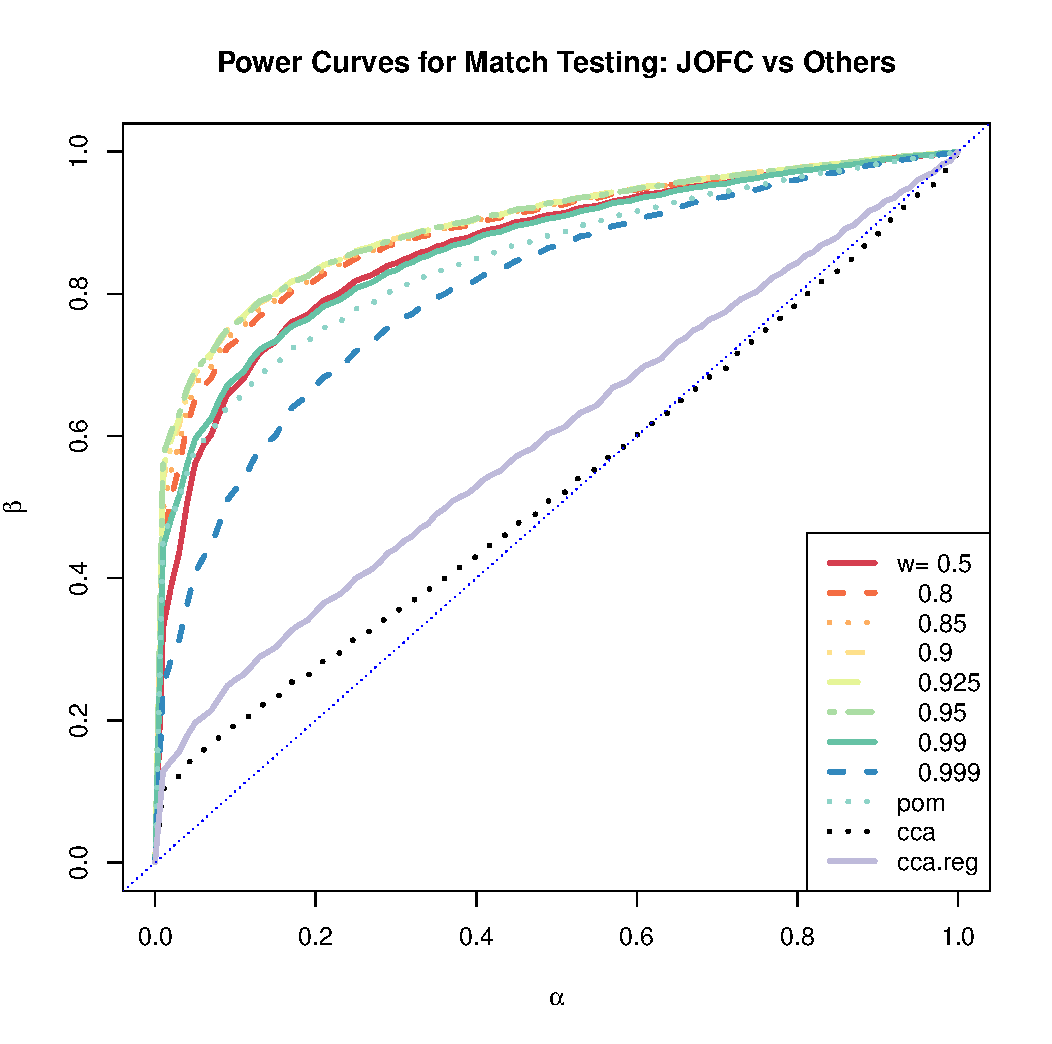
\includegraphics[scale=0.8]{MVN_JOFC_q_90_c_0_001}
\caption{Large Noise Dimension Behaviour of JOFC,P$\circ$ M and CCA approaches}
\label{fig:largeq}
\end{figure}



\section{Experiments on Wiki Data}
To test the JOFC approach with real data, a collection of articles are collected from the English Wikipedia, consisting of the
 directed 2-neighborhood of the document "Algebraic Geometry". 
   This  collection of 1382 articles and the correspondence of each article in French 
Wikipedia is our real-life dataset. It is possible to utilize both textual content of the documents and the hyperlink graph structure. The textual content of the documents is summarized by the bag-of-words model. Dissimilarities between documents  in the same language are computed by the Lin-Pantel discounted mutual information \cite{LinPantel,PantelLin}
 and cosine dissimilarity $k(x_{ik}; x_{jk}) = 1 - (x_{ik} x_{jk})/(\|x_{ik}\|_2\|x_{ik}\|_2)$. 
 The dissimilarities based on the hyperlink graph of the collection of the articles are 
 for each pair of vertices $i$ and $j$, the number of vertices one must travel to go from $i$ to $j$.  Further details about this dataset is available in \cite{Zhiliang_disparate}     
Only  dissimilarities based on the textual content will be considered in this example.
   
The exploitation task is still testing for matchedness of vertices between different conditions, in this case wiki articles that are on the same topic  in  different languages.
For hypothesis testing,   randomly held out four documents - one matched pair and one unmatched pair
 -  are used to compute empirical type I error $\alpha$ and estimate of power based on the critical value computed
  from the distribution of the test statistic for the remaining 1380 matched pairs. 
The test statistic is computed using one of the three approached mentioned  $cca$, $p\circ m$, and $jofc$ . 
The two sets of held-out matched pairs are embedded as $\tilde{y}_1$ and $\tilde{y}_2$, via out-of-sample
embedding, to estimate the null distribution of the test statistic $T = d(\tilde{y}_1; \tilde{y}_2)$. This allows
us to estimate critical values for any specified Type I error level. 
Then the two sets of heldout unmatched pairs are embedded as $\tilde{y'}_1$ and $\tilde{y'}_2$, via out-of-sample embedding. 
$T' = d(\tilde{y'}_1; \tilde{y'}_2)$ will give us an empirical distribution of the test statistic  under the alternative hypothesis. 
And the distribution under null hypothesis and under alternative hypothesis can be used to estimate power.
Target dimensionality d is determined by the Zhu and Ghodsi  automatic dimensionality selection
method \cite{ZhuGhodsi}, resulting in d = 6 for this data set.


\begin{figure}
 \centering
\includegraphics[scale=0.8]{graphs/FidCommPaperwiki-two-cond-plot} 
\end{figure}



\section{Model Selection}
For the simulations presented up to now, the embedding dimension $d$ was set to 2. This was a convenient choice which allowed us to investigate various aspects of JOFC and competing approaches.
However,  more care is required in selection of this parameter, since it plays such a big role in performance in general learning settings. The signal dimension was set to $p=10$ and different $d=2,5,7,10,15$ values were used to test the JOFC approach.
The following plots of ROC curves in    \ref{fig:ROC-d} and  \ref{fig:ROC-d-15} shows the effect of $d$ parameter on the performance of different methods for the Gaussian setting for the noisy case.

\begin{figure}
 \centering
  \captionsetup[subfigure]{labelformat=empty}
        \begin{subfigure}[b]{0.5\textwidth}        
               \centerline{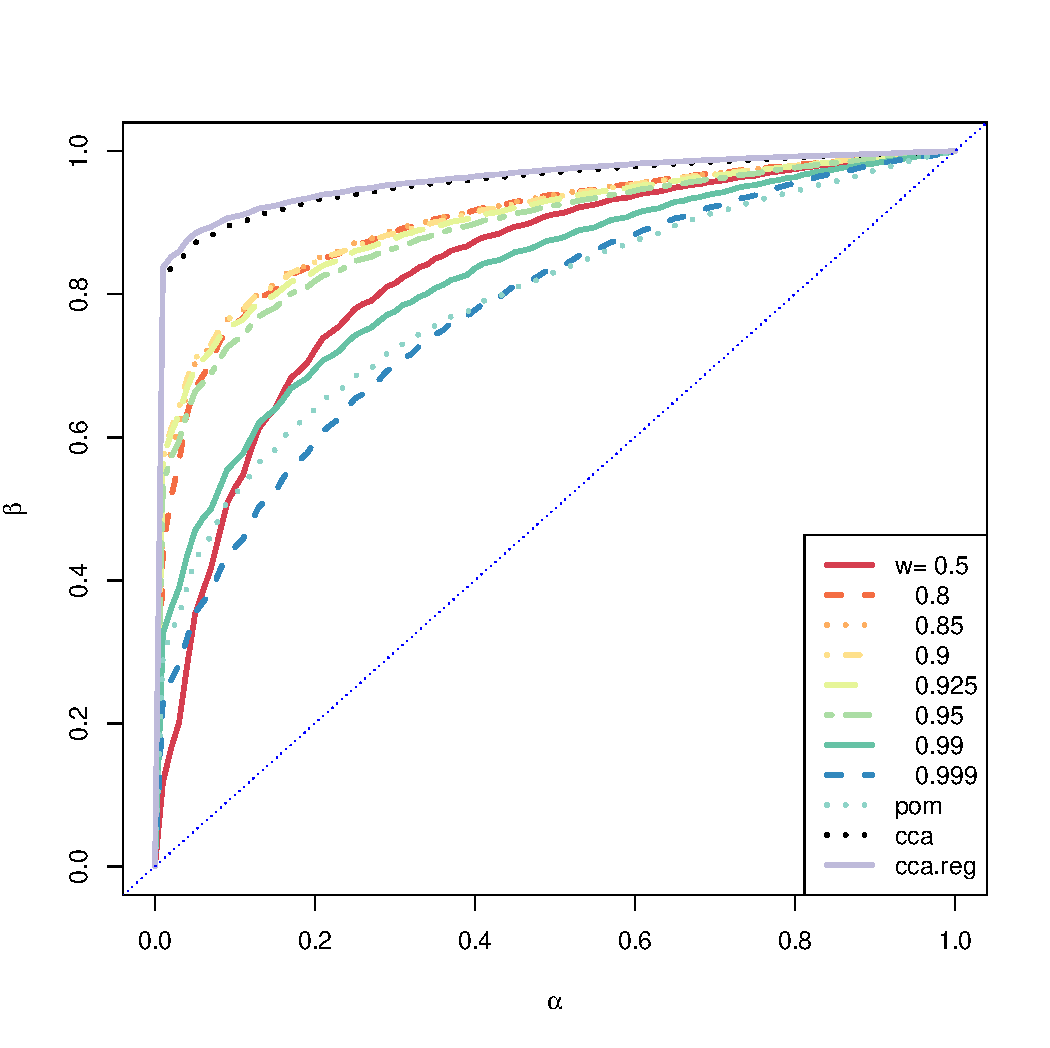
\includegraphics[width=\textwidth]{ROC-d-2.pdf}}
                \caption{d=2}
                \label{fig:ROC-d-2}
        \end{subfigure}%
         %add desired spacing between images, e. g. ~, \quad, \qquad etc. 
          %(or a blank line to force the subfigure onto a new line)
        \begin{subfigure}[b]{0.5\textwidth}           
                  \centerline{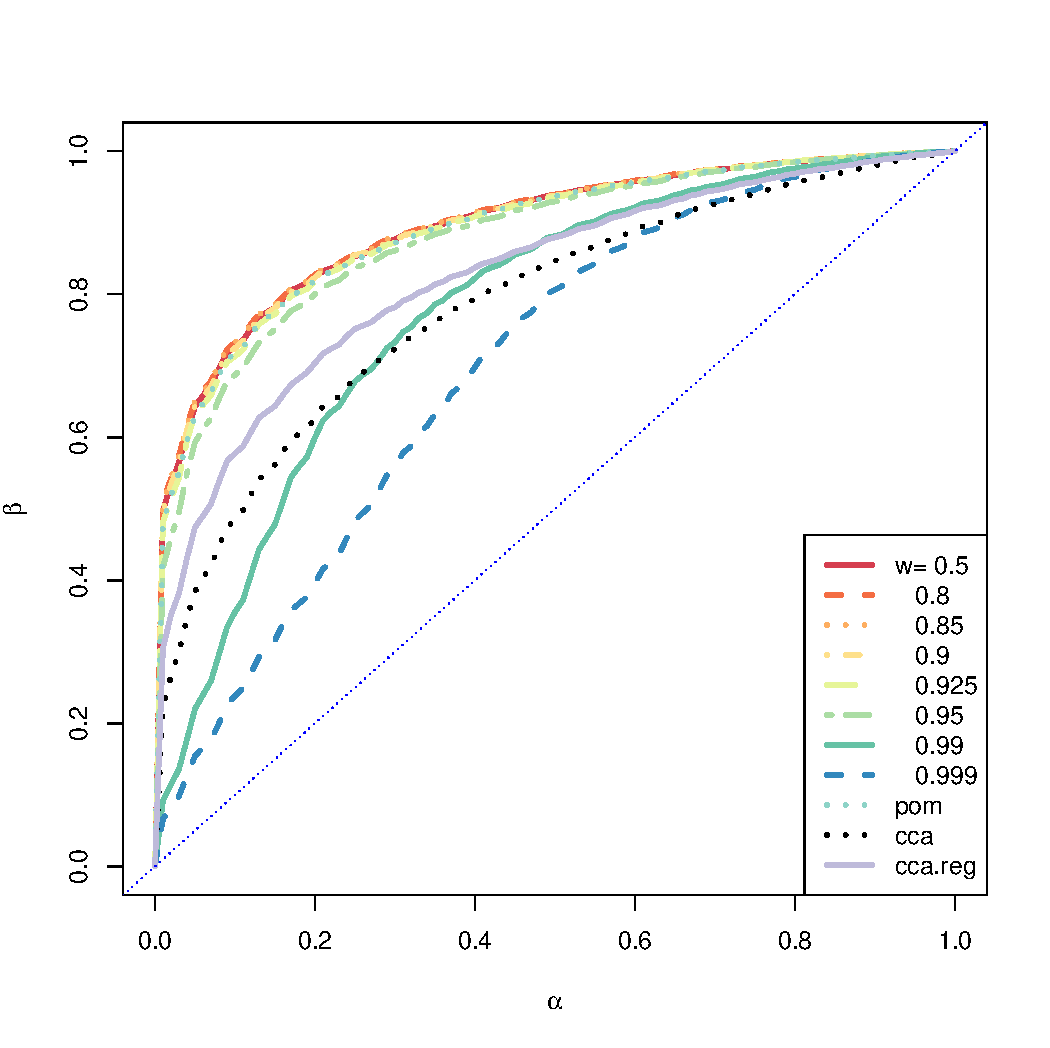
\includegraphics[width=\textwidth]{ROC-d-5.pdf}}
                \caption{d=5}
                \label{fig:ROC-d-5}
        \end{subfigure}      
        %add desired spacing between images, e. g. ~, \quad, \qquad etc.    %(or a blank line to force the subfigure onto a new line)
        \begin{subfigure}[b]{0.47\textwidth}             
               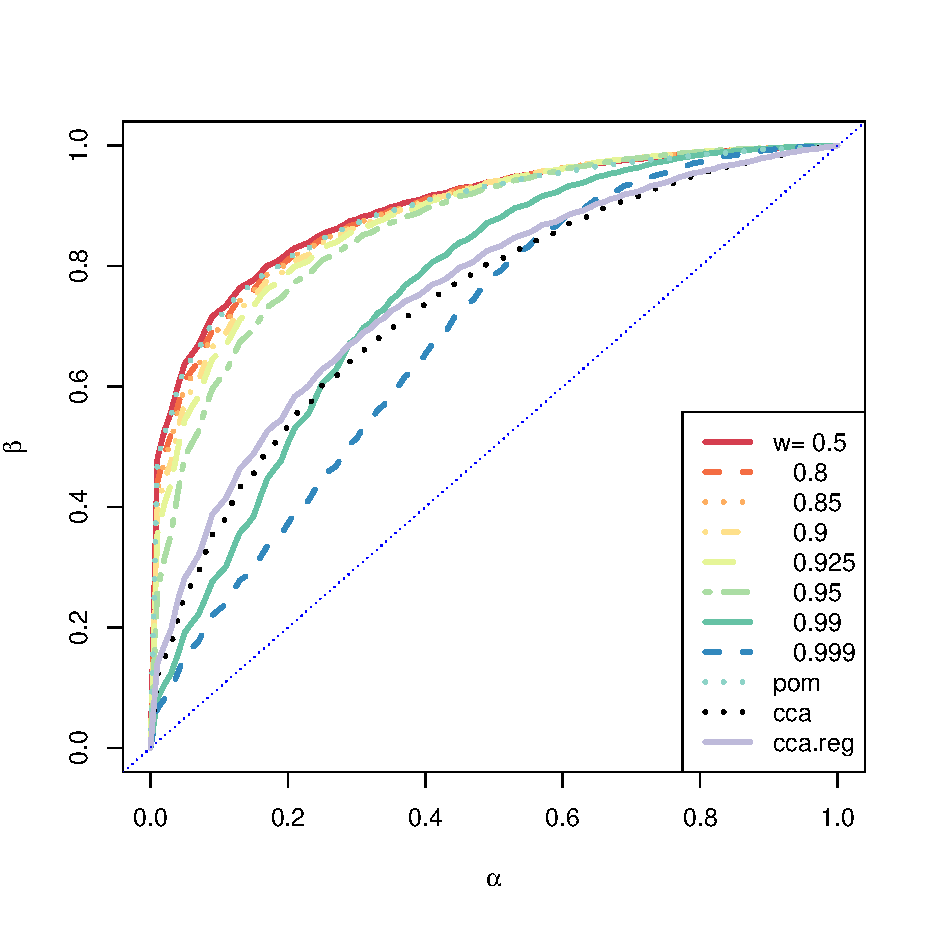
\includegraphics[width=\textwidth]{ROC-d-7.pdf}
                \caption{d=7}
                \label{fig:ROC-d-7}
        \end{subfigure}          
               \begin{subfigure}[b]{0.47\textwidth}
                \centering
               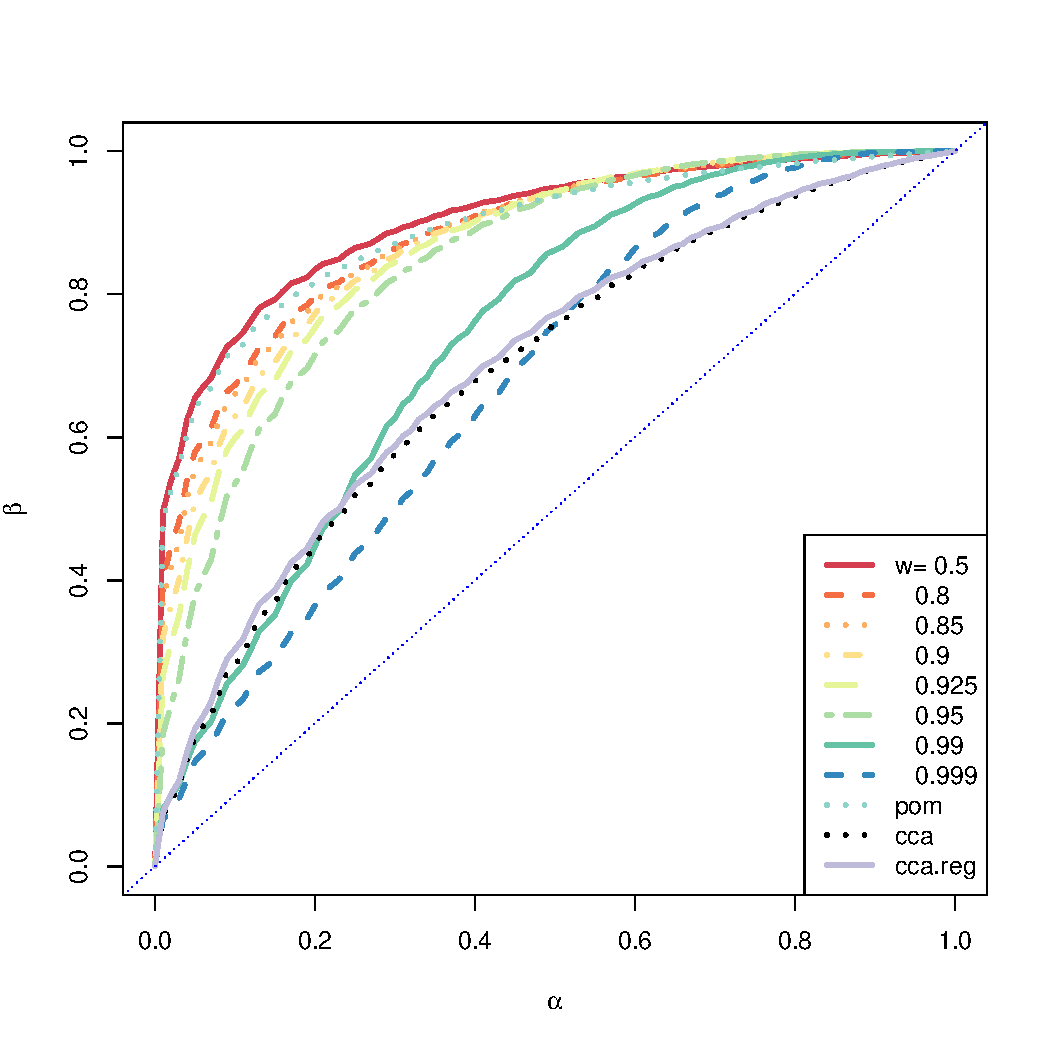
\includegraphics[width=\textwidth]{ROC-d-10.pdf}
                \caption{d=10}
                \label{fig:ROC-d-10}
        \end{subfigure}
         
        \caption{Effect of $d$ parameter on ROC plots}\label{fig:ROC-d}
        \label{fig:ROC-d}

\end{figure}

\begin{center}
\begin{figure}

                \centering
               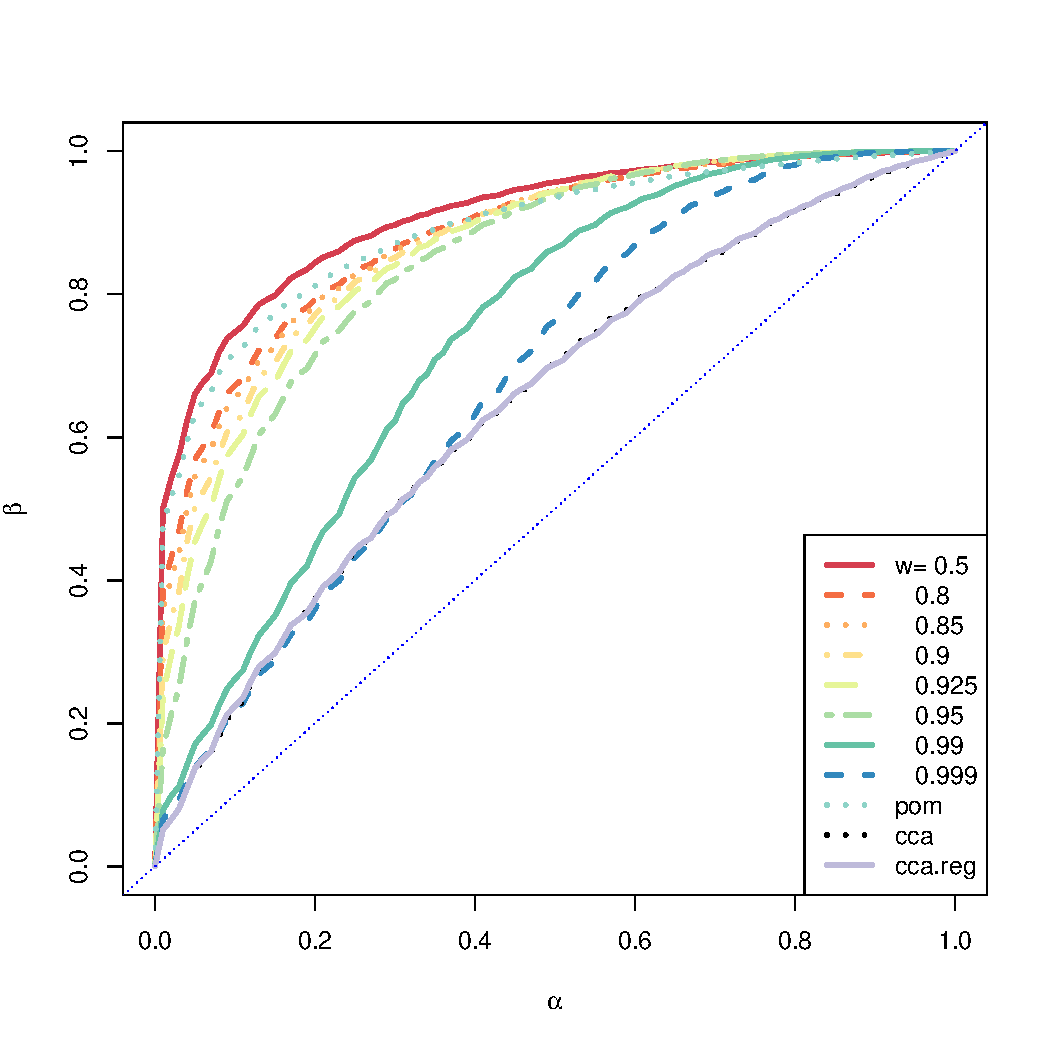
\includegraphics[scale=0.75]{ROC-d-15.pdf}
                \caption{d=15}
                \label{fig:ROC-d-15}
       
\end{figure}
\end{center}










\chapter{Seeded Graph Matching and Fast Approximate Quadratic Programming}
\label{sec:sgm-faq}
\chaptermark{Seeded Graph Matching and Fast Approximate Quadratic Programming }




\section{Experiments on Graph Data}


\section{1-1 matching of vertices}

Another application of  the JOFC approach is  the graph matching problem. For a specific version of this problem, the  inference task is similar to  the same semi-supervised setting as mentioned in \ref{sec:RelatedWork}, where matchings between some vertices in different graphs are known 
  and the task is to infer the correspondences between the remaining collection of vertices in the graphs.  The pairs of vertices whose correspondences are known will be referred to as ``seeds''. We will refer to this variant of the graph matching problem as the ``seeded graph matching'' (SGM) problem.
 
\subsection{Graph Matching }
Consider two  graphs $G_1=(V_1,E_1)$ and $G_2=(V_2,E_2)$ such that $\| V_1 \|=\| V_2 \|=$. Suppose there exists a bijection $f$   such that $f(v_1)=v_2$ and $\forall v' \in \mathbf{N}(v_1) f(v') \in \mathbf{N}(v_2)$. Then the \emph{exact} graph matching problem  is to find this bijection. Even determining the existence  of such an isomorphism is NP-hard.  Although the bijection might not exist,  the \emph{approximate} graph matching problem, which is the task of  finding a bijection between the
graphs which minimizes the degree  of mismatch   between the two graphs, is an interesting problem that has practical applications\cite{GraphMatchReview,Bengoetxea2002,recentdevGraphMatching2000,VogConGraphMatchFAQ,Zaslavskiy2009}.



For the seeded graph matching variant of the problem, additional constraints on $f$ are provided: it must be consitent with the given correspondences, i.e.  $f(v_1)=v_2 for v_1 \in V_1^{*} \subset V_1$ and $v_2 \in V_2$. 

Assume $G_1$ and $G_2$ are unweighted graphs.\footnote{We should note that most of the notation and methods carry over to the weighted case;} It will be convenient to state this problem in terms of adjacency matrices:

Suppose $A,B \in \mathcal{R}^{(r+s)\times (r+s)}$ are adjacency matrices for graphs $G_1$ and $G_2$
 partitioned as ($r$ rows then $s$ rows, $r$ columns then $s$ columns)
\[  A =\left [
\begin{array}{cc} A_{11} & A_{12} \\ A_{21} & A_{22} \end{array} \right ]
\ \ \ \ \ \ \ \ \ B =\left [
\begin{array}{cc} B_{11} & B_{12} \\ B_{21} & B_{22} \end{array} \right ]
\]
To simplify  suppose that $A_{11}=B_{11}$ , ie the first $r$ vertices
of $A$'s graph correspond respectively to the first $r$ vertices of $B$'s graph,
and we wish to complete the isomorphism by determining the correspondences between the pairs of $s$ vertices. 
That is, we seek a permutation matrix $P \in \{0,1\}^{s \times s}$ such that $A=(I_{r \times r}
\oplus P)B(I_{r \times r} \oplus P)^T$, ie
 \[
 \left [
\begin{array}{cc} A_{11} & A_{12} \\ A_{21} & A_{22} \end{array}
\right ]
\left [
\begin{array}{cc} I_{r \times r} & 0_{r \times s} \\ 0_{s \times r} & P \end{array}
\right ]
=
\left [
\begin{array}{cc} I_{r \times r} & 0_{r \times s} \\ 0_{s \times r} & P \end{array}
\right ]
\left [
\begin{array}{cc} B_{11} & B_{12} \\ B_{21} & B_{22} \end{array}
\right ] 
\].  It is obvious that $P$ defines $f$: $V_1 \rightarrow V_2$, the bijection  between the two graphs we are interested in.



For the approximate graph matching problem, we seek $P$ that minimizes $h(P)$, which measures mismatch, as measured by, say $h(.)$, over all bijective functions
For unweighted graphs, the degree of mismatch is characterized by the number of adjacency disagreements, i.e
$h(P)=\|(I_{r \times r}\oplus P)^{T}A(I_{r \times r}\oplus P)-B\|_1$ subject to $P$ being a permutation matrix.
For weighted graphs, it could be any monotonic transformation of the difference between the weights of matching edges.
%Although an efficient algorithm  for the general  graph matching problem is not known, there are various principled heuristic algorithms for  approximate solutions of the graph matching problem  in the literature\cite{GraphMatchReview}.
   
   
 Note this optimization problem is equivalent to minimizing various functions, e.g.
 
$\|A(I_{r \times r}\oplus P)-(I_{r \times r}\oplus P)B\|_1$ (since $I_{r \times r}\oplus P$ is a permutation matrix) or

$\|A-(I_{r \times r}\oplus P)B(I_{r \times r}\oplus P)^T\|_2$ (monotonic function of $\ell_1$ norm) or

$\|A(I_{r \times r}\oplus P)-(I_{r \times r}\oplus P)B\|_2$ ( $I_{r \times r}\oplus P$ is unitary), or 
maximizing 
$\tr {A^T(I_{m \times m}\oplus P)B(I_{m \times m}\oplus P^T)}$ (expanding out $\|A-(I_{m \times m}\oplus P)B(I_{m \times m}\oplus P)^T\|_2^2=
\|A\|_2^2 + \|B\|_2^2
- 2 \cdot \tr{A^T(I_{m \times m}\oplus P)B(I_{m \times m}\oplus P^T)}$  and removing the constant terms)

over all permutation matrices $P$,
where $\| \cdot \|_2$ is the $\ell_2$ vector norm on matrices.   Althought these different formulations  are equivalent, their relaxations result in different methods for solving the approximate graph matching problem\ref{subsec:rqap2}. Specfically the $\ell_1$ formulation is the  linear assignment problem. $\ell_2$ formulations are examples of the quadratic assignment problem.

 


\subsection{Fast approximate quadratic programming for Seeded Graph Matching}


A relaxation of the general   approximate graph matching problem by letting the  domain of $P$ be doubly stochastic matrices can be solved efficiently by successively solving linearizations of the objective function, the Frank-Wolfe Method. We propose the seeded case version of this relaxation (named as fast approximate quadratic programming)  as the solution to the seeded graph matching problem.

A brief review of the Frank-Wolfe method is necessary before we go into FAQ method for Seeded Graph Matching. The FW algorithm solves the following optimization problem: the minimization of a convex and differentiable function, denoted by $h(x)$ 
over a bounded and convex domain $\mathbf{S}$. 

\begin{algorithm}[H]
 \SetAlgoLined
 %\KwData{this text}
 \KwResult{$x^*$}
 $i=1$\;
 
 $\alpha=1$\;
 
 $x^1$ = Random element of   $\mathbf{S}$  or initial estimate of $\mathit{x^*}$ \;
 
 \While{$\hat{\alpha}>\epsilon $ or $\|\nabla{h(x^{i})}\| > \epsilon$ }{
  Solve $\hat{\vec{x}}= \argmin_{\vec{x}}\nabla{h(x^{i})}^{T}\vec{x}$  with respect to  $\vec{x}$. 
  
 Solve  $\hat{\alpha}= \argmin_{\hat{\alpha}}{h(x^{i}+\alpha*(\vec{x}-x^{i}))}$  with $\alpha \in (0,1)$.
 
  Let $x^{i+1}= x^{i}+\hat{\alpha}*\vec{x}$. 
  
  $\mathit{x^*}=x^{i+1}$ 
  
 }
 \caption{Frank-Wolfe algorithm}
\end{algorithm}

The first step in the loop solves a linear approximation of the problem $h(x)=h(x^i)+\nabla{h(x^i)}(x-x^i)$. The second step minimizes the original function with the domain restricted to the line between $\hat{\vec{x}}$ and $x^{i}$ In the case, where $h(x)$ is quadratic, a unique  $\hat{\alpha}$ can be found analytically.

Let us now present the derivation of the steps of  FAQ algorithm.  The relaxation we choose for FAQ is $\tr {A^T(I_{m \times m}\oplus P)B(I_{m \times m}\oplus P^T)}$. This is a simplified expression for $\ell_2$ distance of $A$ and $(I_{m \times m}\oplus P)B(I_{m \times m}\oplus P)^T$. Therefore we call this formulation relaxed quadratic assignment problem (rQAP1).
The objective function is
\begin{eqnarray*}  h(P)  & =  &   \tr \left (
\left [  \begin{array}{cc}  A^T_{11} & A^T_{21} \\ A^T_{12} & A^T_{22}  \end{array} \right ]
\left [  \begin{array}{cc}  I_{r \times r} & 0_{r \times s}
\\ 0_{s \times r} & P  \end{array} \right ]
\left [  \begin{array}{cc}  B_{11} & B_{12} \\ B_{21} & B_{22}  \end{array} \right ]
\left [  \begin{array}{cc}  I_{r \times r} & 0_{r \times s}
\\ 0_{s \times r} & P^T  \end{array} \right ]
\right ) \\
& = & \tr \left (
\left [  \begin{array}{cc}  A^T_{11} & A^T_{21} \\ A^T_{12} & A^T_{22}  \end{array} \right ]
\left [  \begin{array}{cc}  B_{11} & B_{12}P^T \\ PB_{21} & PB_{22}P^T  \end{array} \right ]
\right )\\
& = & \tr A_{11}^TB_{11}+ \tr A_{21}^TPB_{21}+\tr A_{12}^TB_{12}P^T
+ \tr A_{22}^TPB_{22}P^T \\
& = &  \tr A_{11}^TB_{11}+ \tr P^T A_{21}B_{21}^T+\tr P^TA_{12}^TB_{12}
+ \tr A_{22}^TPB_{22}P^T
\end{eqnarray*}
which has gradient which is presented in matrix form as 
\begin{eqnarray*}
Grad(P):=A_{21}B_{21}^T+A_{12}^TB_{12}+A_{22}PB_{22}^T+A_{22}^TPB_{22} .
\end{eqnarray*}. Note that $h(P)$ has a quadratic form with respect to $P$ which will help us in the second step of F-W iterations.


In our experiments,  the Frank-Wolfe Algorithm was initialized with
$\tilde{P}=\frac{1}{s}\vec{1}_{s} \vec{1}_{s}^T$. (This initialization is arbitrary , a random $\tilde{P}$ can be chosen). 

Now we adapt F-W algorithm to the minimization of $h(P)$.  For each iteration $i$, in the first step let $\tilde{P}^{i}$ the current estimate of $P$. We are supposed to compute  $Q$ which would minimize  $-\tr Q^{T}Grad(\tilde{P}^{i})$ over all $s \times s$ doubly stochastic matrices $Q \in \M ^{s \times s}$. Equivalently $\tr Q^{T}Grad(\tilde{P}^{i})$ is maximized with respect to $Q$. We will use  $\nabla$ in place of $Grad(\tilde{P}^{i})$.
Note that $\hat{Q}$ can be assumed to be a permutation matrix.  To see this, assume $\hat{Q}$ is not a permutation matrix and there exist a row ,say $i^{th}$ of $\hat{Q}$, $q_i$ that is not a canonical basis. Note that the contribution of $q_{i}$ to trace of $Q^{T}G(\tilde{P}^{i})$ is $\sum_{k}{q_{ik}\nabla{}_{ki}}$. Subject to $\sum_{k}{q_{ik}}=1$. Note that $Q^{*}$ such that $Q_{io}^{*}=1$,  $Q_{ik}^{*}=1$ for $k \neq o$ for $o=\argmax_k{\nabla{}_{ki}}$  $Q_{mn}^{*}=\hat{Q}_{mn}$ for $m=$
Therefore , the  Hungarian Algorithm will in fact find the optimal $Q$, call it
$\hat{Q}$.
The next task in the Frank-Wolfe algorithm step
will be maximizing the objective function over the line
segment from $\tilde{P}^{i}$ to $\hat{Q}$;  ie maximizing $z(\alpha):=h(\alpha \tilde{P}
+(1-\alpha ) \hat{Q})$ over $\alpha \in [0,1]$. Denote
$c:=\tr A^T_{22} \tilde{P} B_{22} \tilde{P}^T$ and
$d:=\tr (A^T_{22} \tilde{P} B_{22} \tilde{Q}^T +
    A^T_{22} \tilde{Q} B_{22} \tilde{P}^T)$ and
$e:=\tr A^T_{22} \tilde{Q} B_{22} \tilde{Q}^T$ and
$u:=\tr ( \tilde{P}^TA_{21}B_{21}^T   + \tilde{P}^TA_{12}^TB_{12} )$ and
$v:=\tr ( \tilde{Q}^TA_{21}B_{21}^T   + \tilde{Q}^TA_{12}^TB_{12} )$. Then
(ignoring the additive constant $\tr A_{11}^TB_{11}$ without loss of
generality)
we have $z(\alpha)=c \alpha^2+d \alpha (1-\alpha)
+e(1-\alpha)^2+u \alpha + v(1-\alpha)$  which simplifies to
$z(\alpha)=(c-d+e)\alpha^2+(d-2e+u-v)\alpha + (e+v)$. Setting the
derivative of $z$ to zero yields potential critical point
$\hat{\alpha}:=\frac{-(d-2e+u-v)}{2(c-d+e)}$ (if indeed
$0 \leq \hat{\alpha}\leq 1$). 
If $\hat{\alpha}>\epsilon$, the algorithm terminates that is $\hat{P}=\tilde{P}^{i}$ as it has reached a local minimum. Otherwise, we set $\tilde{P}^{i+1}= \hat{\alpha} \tilde{P}^{i}
+(1- \hat{\alpha} ) \hat{Q}$ if $\hat{\alpha}>\epsilon$   and repeat the steps for the next iteration.
At the termination of the Frank-Wolfe Algorithm, it is quite possible that   ${P}^{*}$ is not a permutation matrix. One way to get a permutation matrix solution is to find  ${\tilde{P}}^{*}$ that is as close as possible to  ${P}^{*}$ (in some sense).  Note that in discussion of the different formulations of the  original optimization problem, we showed that maximizing $2*\tr {ST}$ with respect to $S$ was equivalent to minimizing $\ell_2$ distance between $S$ and $T$, and we have shown, in the discussion of the FAQ algorithm, minimization of  $2*\tr {ST}$ is solved by the Hungarian algorithm when $S$ is constrained to be permutation matrix. Therefore we can use the Hungarian algorithm one last time to get a permutation matrix result by  minimizing ${\tilde{P}}^{*}{P}^{*}$ with respect to ${\tilde{P}}^{*}$  which is the closest permutation matrix to  ${{P}}^{*}$ in $\ell_2$ sense.



\subsection{Relaxations of alternate formulations of the approximate seeded graph matching problem \label{subsec:rqap2}}

There is another quadratic assignment problem formulation of  the approximate seeded graph matching problem, where the objective function is  minimized. We call this formulation rQAP2.
The objective function for rQAP2 is
$\|A(I_{m \times m}\oplus P)-(I_{m \times m}\oplus P)B\|$. If one applies the constraint $\|PX\|=\|X\|$ for any permutation matrix $P$, this function simplifies to minimum of -2 times the objective function of  rQAP.

\begin{align*}
f(P) & = & \lVert AP^{*}-P^{*}B\rVert _{F}\\
 & = & \left\Vert A_{21}-PB_{21}\right\Vert _{F} & + & \left\Vert A_{12}P-B_{12}\right\Vert _{F} & +\left\Vert A_{22}P-PB_{22}\right\Vert _{F} & \textrm{Terms (1), (2) and (3)}
\end{align*}


where $P^{*}$ is the omnibus permutation matrix $\left[\begin{array}{cc}
I & \mathbf{0}\\
\mathbf{0} & P
\end{array}\right]$ .


Consider term (1)

\begin{align*}
\left\Vert A_{21}-PB_{21}\right\Vert _{F} & = & \tr\left[\left(A_{21}-PB_{21}\right)^{T}\left(A_{21}-PB_{21}\right)\right]\\
 & = & \tr\left[A_{21}^{T}A_{21}-B_{21}^{T}P^{T}A_{21}-A_{21}^{T}PB_{21}+B_{21}^{T}P^{T}PB_{21}\right]\\
 & = & \tr\left[A_{21}^{T}A_{21}-B_{21}^{T}P^{T}A_{21}-A_{21}^{T}PB_{21}+P^{T}PB_{21}B_{21}^{T}\right]\\
 & = & \tr\left[A_{21}^{T}A_{21}-2*B_{21}^{T}P^{T}A_{21}+P^{T}PB_{21}B_{21}^{T}\right]
\end{align*}


where the simplification in the last line is due to the fact that
the matrices with minus signs in front are transposes of each other.
The three terms inside the brackets in the last line are referred
as (1.1),(1.2) and (1.3), respectively.

Similarly for term (2)

\begin{align*}
\left\Vert A_{12}P-B_{12}\right\Vert _{F} & = & \tr\left[\left(A_{12}P-B_{12}\right)^{T}\left(A_{12}P-B_{12}\right)\right]\\
 & = & \tr\left[P^{T}A_{12}^{T}A_{12}P-B_{12}^{T}A_{12}P-P^{T}A_{12}^{T}B_{12}+B_{12}^{T}B_{12}\right]\\
 & = & \tr\left[PP^{T}A_{12}^{T}A_{12}-B_{12}^{T}A_{12}P-P^{T}A_{12}^{T}B_{12}+B_{12}^{T}B_{12}\right]\\
 &  & \tr\left[PP^{T}A_{12}^{T}A_{12}-2P^{T}A_{12}^{T}B_{12}+B_{12}^{T}B_{12}\right]
\end{align*}


The three terms inside the brackets are referred as (2.1),(2.2) and
(2.3), respectively.

and finally term (3)

\begin{align*}
\left\Vert A_{22}P-PB_{22}\right\Vert _{F} & = & \tr\left[\left(A_{22}P-PB_{22}\right)^{T}\left(A_{22}P-PB_{22}\right)\right]\\
 & = & \tr\left[P^{T}A_{22}^{T}A_{22}P-B_{22}^{T}P^{T}A_{22}P-P^{T}A_{22}^{T}PB_{22}+B_{22}^{T}P^{T}PB_{22}\right]\\
 & = & \tr\left[PP^{T}A_{22}^{T}A_{22}-B_{22}^{T}P^{T}A_{22}P-P^{T}A_{22}^{T}PB_{22}+PB_{22}B_{22}^{T}P^{T}\right]
\end{align*}


The three terms inside the brackets are referred as (3.1),(3.2) ,(3.3)
and (3.4), respectively.

Note that $\tr\left[PP^{T}A_{22}^{T}A_{22}-B_{22}^{T}P^{T}A_{22}P-P^{T}A_{22}^{T}PB_{22}+PB_{22}B_{22}^{T}P^{T}\right]$
can be further simplified to 

\[
\tr\left[PP^{T}A_{22}^{T}A_{22}-2*P^{T}A_{22}^{T}PB_{22}+PB_{22}B_{22}^{T}P^{T}\right]
\]
.


The gradient for rQAP2 with hard seeds (minimization problem) is

$\nabla_{P}f(P)=-2A_{21}B_{21}^{T}+2PB_{21}B_{21}^{T}-2A_{12}^{T}B_{12}+2A_{12}^{T}A_{12}P+2(A_{22}^{T}A_{22}P+PB_{22}B_{22}^{T}-A_{22}^{T}PB_{22}-A_{22}PB_{22}^{T}$)

\begin{flushleft}
The corresponding line search function in terms of $\alpha$ is
\par\end{flushleft}

\begin{flushleft}
\begin{align*}
g(\alpha) & = & \alpha^{2} & \tr\biggl[\hat{P}^{T}\hat{P}\left(B_{21}B_{21}^{T}+B_{22}B_{22}^{T}\right)+\left(A_{12}^{T}A_{12}+A_{22}^{T}A_{22}\right)\hat{P}\hat{P}^{T} & (1.3+3.4)+(2.1+3.1)\\
 &  &  & -\hat{P}^{T}A_{22}^{T}\hat{P}B_{22}-\hat{P}^{T}A_{22}\hat{P}B_{22}^{T}\biggr] & -(3.2)-(3.3)\\
 & + & \left(1-\alpha\right)^{2} & \tr\biggl[\hat{Q}^{T}\hat{Q}\left(B_{21}B_{21}^{T}+B_{22}B_{22}^{T}\right)+\left(A_{12}^{T}A_{12}+A_{22}^{T}A_{22}\right)\hat{Q}\hat{Q}^{T} & (1.3+3.4)+(2.1+3.1)\\
 &  &  & -\hat{Q}^{T}A_{22}^{T}\hat{Q}B_{22}-\hat{Q}^{T}A_{22}\hat{Q}B_{22}^{T}\biggr] & -(3.2)-(3.3)\\
 & + & \alpha\left(1-\alpha\right) & \tr[\left(\hat{Q}^{T}\hat{P}+\hat{P}^{T}\hat{Q}\right)\left(B_{21}B_{21}^{T}+B_{22}B_{22}^{T}\right)+\left(A_{12}^{T}A_{12}+A_{22}^{T}A_{22}\right)\left(\hat{Q}\hat{P}^{T}+\hat{P}\hat{Q}^{T}\right) & (1.3)+(3.4)+(2.1)+(3.1)\\
 &  &  & -\hat{P}^{T}\left[A_{22}^{T}\hat{Q}B_{22}+A_{22}\hat{Q}B_{22}^{T}\right]-\hat{Q}^{T}\left[A_{22}^{T}\hat{P}B_{22}+A_{22}\hat{P}B_{22}^{T}\right]] & -[(3.3)+(3.2)]-[(3.3)+(3.2)]\\
 & + & \alpha & \tr\left[-2\hat{P}B_{12}^{T}A_{12}-2\hat{P}^{T}A_{21}B_{21}^{T}\right] & [-(2.2)-(1.2)]\\
 & + & \left(1-\alpha\right) & \tr\left[-2\hat{Q}B_{12}^{T}A_{12}-2\hat{Q}^{T}A_{21}B_{21}^{T}\right] & [-(2.2)-(1.2)]
\end{align*}

\par\end{flushleft}

where the decimal numbers in the right end of the line refer to the
terms for corresponding to $\left\Vert A_{21}-PB_{21}\right\Vert _{F}$
,$\left\Vert A_{12}P-B_{12}\right\Vert _{F}$ and $\left\Vert A_{22}P-PB_{22}\right\Vert _{F}$
in the objective function. Writing $g\left(\alpha\right)$ in terms
of $\alpha$ and (1-$\alpha$),

$g\left(\alpha\right)=c\alpha^{2}+e(1-\alpha)^{2}+d\alpha(1-\alpha)+u\alpha+v(1-\alpha)$

So $c=\tr\left[\hat{P}^{T}\hat{P}\left(B_{21}B_{21}^{T}+B_{22}B_{22}^{T}\right)+\left(A_{12}^{T}A_{12}+A_{22}^{T}A_{22}\right)\hat{P}\hat{P}^{T}-\hat{P}^{T}A_{22}^{T}\hat{P}B_{22}-\hat{P}^{T}A_{22}\hat{P}B_{22}^{T}\right]$

\noindent 
\begin{eqnarray*}
d & = & \tr\biggl[\left(\hat{Q}^{T}\hat{P}+\hat{P}^{T}\hat{Q}\right)\left(B_{21}B_{21}^{T}+B_{22}B_{22}^{T}\right)+\left(A_{12}^{T}A_{12}+A_{22}^{T}A_{22}\right)\left(\hat{Q}\hat{P}^{T}+\hat{P}\hat{Q}^{T}\right)\\
 &  & -\hat{P}^{T}\left[A_{22}^{T}\hat{Q}B_{22}+A_{22}\hat{Q}B_{22}^{T}\right]-\hat{Q}^{T}\left[A_{22}^{T}\hat{P}B_{22}+A_{22}\hat{P}B_{22}^{T}\right]\biggr]
\end{eqnarray*}


$e=\tr\left[\hat{Q}^{T}\hat{Q}\left(B_{21}B_{21}^{T}+B_{22}B_{22}^{T}\right)+\left(A_{12}^{T}A_{12}+A_{22}^{T}A_{22}\right)\hat{Q}\hat{Q}^{T}-\hat{Q}^{T}A_{22}^{T}\hat{Q}B_{22}-\hat{Q}^{T}A_{22}\hat{Q}B_{22}^{T}\right]$

$u=\tr\left[-2\hat{P}B_{12}^{T}A_{12}-2\hat{P}^{T}A_{21}B_{21}^{T}\right]$

$v=\tr\left[-2\hat{Q}B_{12}^{T}A_{12}-2\hat{Q}^{T}A_{21}B_{21}^{T}\right]$

Putting this polynomial of $\alpha$ in standard form, we get $a=c+e-d$,
$b=d-2e+u-v$ and $c=e+v$ .

Note that if this rQAP2 formulation is further simplified  by the unitary property of permutation  matrix, we get the first rQAP formulation. When we use the constraints $P^TP=PP^T=I_{s}$, specific terms in $\nabla_{P}f(P)$ vanish,
$\nabla_{P}f(P)=-2A_{21}B_{21}^{T}+2PB_{21}B_{21}^{T}-2A_{12}^{T}B_{12}+2A_{12}^{T}A_{12}P+2(A_{22}^{T}A_{22}P+PB_{22}B_{22}^{T}-A_{22}^{T}PB_{22}-A_{22}PB_{22}^{T}$
becomes $-2*(A_{21}B_{21}^T+A_{12}^TB_{12}+A_{22}PB_{22}^T+A_{22}^TPB_{22})$
The stronger condition of minimization over the set of permutation matrices is incorporated in the Hungarian Algorithm step.
An interesting question is how does this extra constraint effect the convergence properties of Frank-Wolfe algorithm.  This question is investigated in the comparison of rQAP and rQAP2 formulations.  

\subsection{The comparison of rQAP against the alternative formulation rQAP2}
Although the two formulations are equivalent and the global extrema of the two functions are the same, we expect different convergence  properties. In particular the extra terms in the gradient of rQAP2 which vanishes for unitary matrices should act as a random noise. The conclusion of the literature of stochastic optimization  is that, under some conditions, such noise speeds up convergence, by overcoming local extrema. The problem is that, such noise needs to vanish to negligible levels in order for the iterative algorithm to converge. 
The experiment in the last  section was repeated with both rQAP and rQAP2 and the fraction of nonseed vertices correctly matched and the average number of iterations to satisfy a stopping criteria was compared between the two formulations. 

\begin{figure}
 \centering
  \caption{Fraction of the $n=70$ nonseeds correctly matched using our $\ell_2$-based algorithm for rQAP and rQAP2 formulations
 \label{figell2}}
 \includegraphics[width=1.2\textwidth]{rQAP_vs_rQAP2-alotmore.pdf}
\end{figure}
Note that for small number of hard seeds $rQAP2$ is slighly better, while for larger number of hard seeds $rQAP$ is clearly better. The average number of iterations of Frank-Wolfe algorithm until termination for the two formulation is as follows,

Our conclusion is that our expectations for the two formulations is warranted, rQAP2   converges slower(or doesn't converge, but stays within the neighborhood of the extrema), whiler rQAP converges in very few steps. When the number of hard seeds is small (which corresponds to lower number of constraints for P and higher incidence of local minima near the true solution. ), rQAP2 is slightly better than rQAP.


A natural follow-up to the previous inquiry is whether one can get the best of both world by making a hybrid of the two formulations: First start with minimizing rQAP2 function, until the current iterate of solution is relatively close to the true solution, and follow with maximizing rQAP function. 


\subsection{A hybrid formulation: Fast approximate quadratic programming with smooth transition from rQAP2 to rQAP \label{subsec:hybrid}}

For this hybrid form of the FAQ algorithm, we weight the terms that differ between rQAP2 and rQAP by a decreasing weight $r$. $\nabla_{P}f(P)=
r*\{2PB_{21}B_{21}^{T}
+2A_{12}^{T}A_{12}P
+A_{22}^{T}A_{22}P
+PB_{22}B_{22}^{T}\}
-2A_{21}B_{21}^{T}-2A_{12}^{T}B_{12}
-2A_{22}^{T}PB_{22}-2A_{22}PB_{22}^{T}$. As $r \rightarrow 0 $, the gradient expression at each step of F-W algorithm approaches
$-2*(A_{21}B_{21}^T+A_{12}^TB_{12})+A_{22}PB_{22}^T+A_{22}^TPB_{22})$ which is -2 times the gradient in rQAP. We let $r= 0.5- \frac{\tan((i-(i_{end}/2)))}{\pi}$, so as the iteration counter, $i$ goes from $1$ to $i_{end}$, $r$ goes from $1$ to $0$. This hybrid formulation will behave like rQAP2 for the initial iterations of Frank-Wolfe algorithm and will start to behave like rQAP as $i$ approaches $i_{end}$.


\begin{figure}
 \centering
  \caption{
 \label{fig:hybrid}}
 \includegraphics[width=1.2\textwidth]{sim_bitflip_hybrid_cluster_300_hsv.pdf}
\end{figure}



\chapter{JOFC Approach as a solution to Seeded Graph Matching and comparison to FAQ}
\label{sec:sgm-jofc}
\chaptermark{Seeded Graph Matching and JOFC}


Let us now explain the relevance of JOFC to the graph matching problem. The  task of finding vertex correspondences is similar to  detecting matched pairs in that both of the tasks require the quantification of distance between vertex pairs  in the two graphs.
Using omnibus  embedding, it is possible to embed the vertices of two graphs in a commensurate space.
Therefore, the JOFC approach can be used here for determining the pairwise distances in the commensurate space between  the vertices of $A$ and $B$.
The next step is to use the pairwise distances as costs to find the optimal 1-1 matchings by the Hungarian algorithm \cite{Hung-algo}. The Hungarian algorithm finds an optimal matching between two sets of vertices such that the total  cost which is the sum of the pairwise distances of matched nodes is minimized. This matching step is independent of the embedding, so by always using the Hungarian algorithm, we could investigate what embedding methods are appropriate for the graph matching task and compare  different parameters for the JOFC approach on a equal footing.

 
One useful property of dissimilarity representation is that the structure of data is irrelevant once an appropriate dissimilarity function  for the data is available. 
There are many dissimilarities that can be defined between vertices in graphs. We assume that an appropriate dissimilarity measure is available to us.
In our experiments we will use five different dissimilarities/distances between vertices in a graph:
\begin{itemize}
 \item the shortest path on the  unweighted graph whose adjacency matrix is available
 \item the shortest path on a weighted version of the graph whose adjacency matrix is available
 \item diffusion distance between vertices on the (unweighted) graph.
 \item weighted extension of Czekanowski-Dice dissimilarity\cite{DICE,weightedDICE} which simplifies to the original Czekanowski-Dice dissimilarity (C-D dissimilarity  quantifies local similarity of two vertices in a graph).
 \item expected commute time for random walks on the graph.
 \end{itemize}
 We will omit the results for weighted graph dissimilarities, since they seem to have the same performance as the weighted dissimilarities.
 
 Note that these dissimilarities can only be defined between vertices of the same graph. We impute the inter-condition dissimilarities   as described before in section \ref{omnibus}.
 
\section{Demonstrations}

We perform simulations with graphs, and experiments on real-life graphs for  both modified FAQ approach and JOFC. The performance measure we consider is the true match ratio: the number of true matchings of vertices  divided by the number of pairs of vertices.

\subsection{Simulations}
  To test graph matching approaches, consider the following simulation: $A$ is the adjacency matrix of an Erdos-Renyi graph, that is
  $\left[A\right]_{ij} \sim Binomial(p)$ where $\left[A\right]_{ij}$ is $ij$-th entry of the adjacency matrix  $A$.
 
   and the adjacency matrix  $B$ is a entry-wise bit-flipped version of the adjacency matrix of $A$, that is
   $\left[B\right]_{ij}|\left[A\right]_{ij}=0 \sim Binomial(p_{10})$ $\left[B\right]_{ij}|\left[A\right]_{ij}=1 \sim Binomial(p_{11})$. Suppose $p_{10}=p_{11}=p$.
  
  The probability of flipping an entry of the adjacency matrix is the perturbation parameter $p_{pert}$ which is the variable on the x-axis. 
  The performance measure is the proportion of true matches to the number of matches. Note that 
  under chance, the expected number of true matches is 1, as shown with the dashed line. In this particular simulation, we consider the JOFC approach with classical and raw stress variants and compare the performance of each in small graphs. $r=20$ and $s=5$. $p_{pert}$ varies from $0$ to $1$ in increments of $0.1$.  
  
\begin{figure}
  \includegraphics[scale=0.65]{FidCommPapergraph-plot-1.pdf}
\end{figure}












Note that JOFC for unweighted and weighted graphs  have better performance compared to CMDS. As the perturbation parameter gets larger, the performance degrades until it is indistinguishable from random chance at $pert=0.5$.

\begin{comment}
Another feature of the plot is the U-shape of the curve for diffusion-distance based dissimilarities. This invariancy with respect to complement of the graph should be investigated further.

\includegraphics{graphs/FidCommPapergraph-plot-3}An interesting trend in the graph is that shortest-path based dissimilarities are an improvement over diffusion-path dissimilarities for perturbation parameter less than 0.5 , but as perturbation parameter increases past 0.5, fraction of correct matches for diffusion distance based dissimilarity recovers, while for other dissimilarities the fraction continues to fall. 
\end{comment}

 
  To test JOFC approach, consider the following simulation: $A$ is the adjacency matrix of an Erdos-Renyi graph, that is
  $\left[A\right]_{ij} \sim Binomial(p)$ where $\left[A\right]_{ij}$ is $ij$-th entry of the adjacency matrix  $A$.
   and the adjacency matrix  $B$ is a entry-wise bit-flipped version of the adjacency matrix of $A$, that is
    $\left[B\right]_{ij}|\left[A\right]_{ij}=0 \sim Binomial(p_{10})$ $\left[B\right]_{ij}|\left[A\right]_{ij}=1 \sim Binomial(p_{11})$. Suppose $p_{10}=p_{11}=p_{pert}$.
  
  The probability of flipping an entry of the adjacency matrix is the perturbation parameter $p_{pert}$ which is the variable on the x-axis. 
  The performance measure is the proportion of true matches to the number of matches. Note that 
  under chance, the expected number of true matches is 1, as shown with the dashed line. In the simulation, $r=20$ and $s=5$. $p_{pert}$ varies from $0$ to $1$ in increments of $0.1$. 
\begin{figure}
  \includegraphics[scale=0.65]{FidCommPapergraph-plot-1.pdf}
\end{figure}


In the plot above, JOFC approach applied to  dissimilarities based on weighted and unweighted graphs is compared with classical MDS on dissimilarities of weighted graphs.

As the perturbation parameter gets larger, the performance degrades until it is indistinguishable from random chance at $pert=0.5$.

Another feature of the plot is the U-shape of the curve for diffusion-distance based dissimilarities. This invariancy with respect to complement of the graph should be investigated further.

  

\begin{figure}
\centering
\includegraphics{graphs/FidCommPapergraph-plot-3} 
\end{figure}



An interesting trend in the graph is that shortest-path based dissimilarities are an improvement over diffusion-path dissimilarities for perturbation parameter less than 0.5 , but as perturbation parameter increases past 0.5, fraction of correct matches for diffusion distance based dissimilarity recovers, while for other dissimilarities the fraction continues to fall. 

The dissimilarity type that has the best improvement in performance is JOFC with shortest path distances in weighted graphs(unweighted graphs have similar performance).



This graph shows the effect of the weight parameter of stress $w$ on the probability of true matches.
\begin{figure}
\includegraphics{FidCommPaper-graph-plot-4}
\end{figure}
There are a lot  of interesting questions to ponder about the number of known correspondences, such as , how many known correspondences are necessary for satisfactory performance for graphs of some fixed size and whether , in the ``match ratio'' vs number of known correspondences curve,  there are any ``elbows'' , after which the cost of more correspondences are not justified by the accompanying increase in ``match ratio''. Figure \ref{bitflipJOFC} shows ``match ratio'' plotted against number of ``seeds'' for the same bitflip experiments using  Czekanowski-Dice dissimilarities . These results suggest that even with the perturbation, when a portion of the correspondences are known, it is possible to recover most of the remaining correspondences. This application of JOFC is  investigated further in \cite{SGMviaJOFC} with real datasets.
\begin{figure}
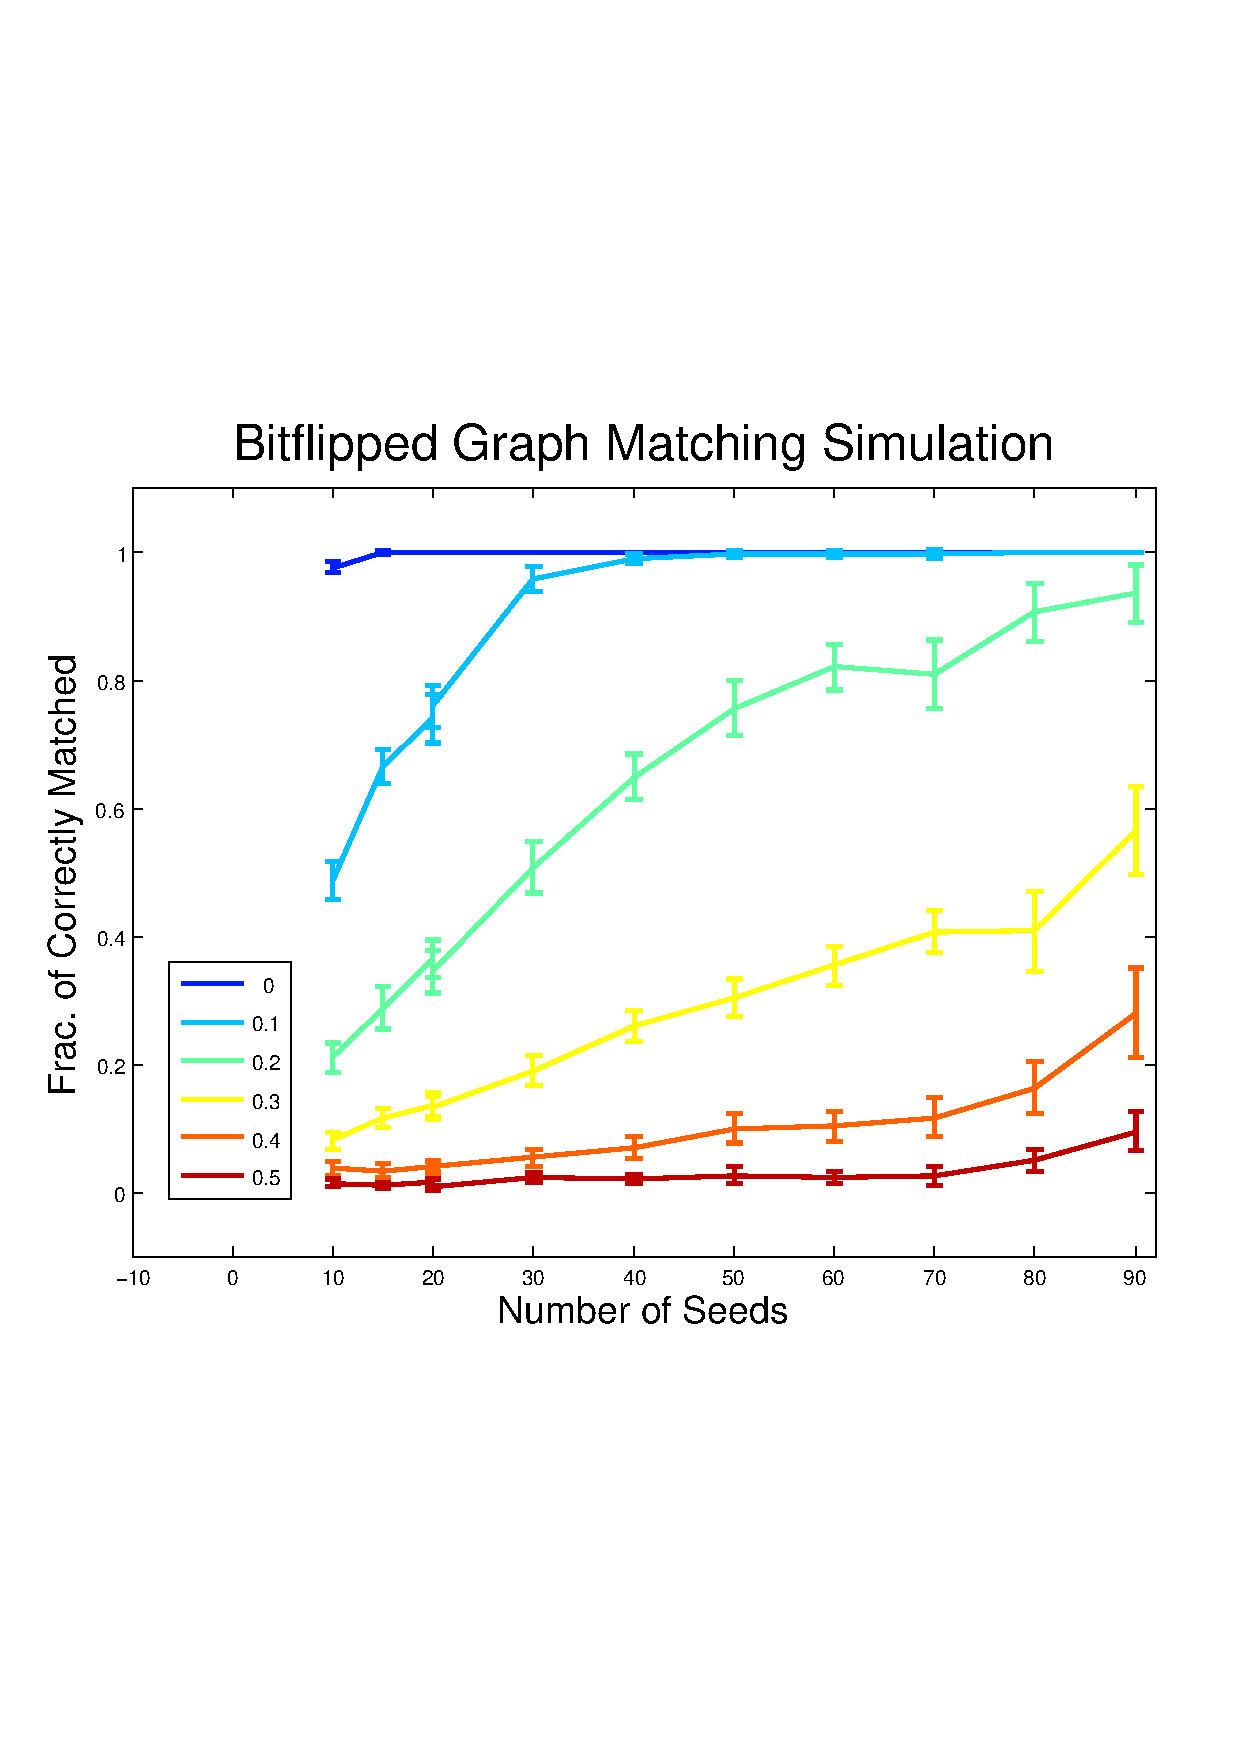
\includegraphics[scale=0.75]{bitflip_JOFC}
\caption{Bitflip Simulations for JOFC \label{bitflipJOFC}}
\end{figure}


\subsection{Experiments on Real data}

\subsubsection{C. elegans connectome}
For experimental data, we consider two connectivity graphs of 279 neurons in the  worm C. elegans. The two conditions are two ways of measuring connectivity among neurons. The  weight matrix for the first connectivity type is Ac which is not symmetric, has values between 0 and 37 and is relatively sparse (has 2194 non-zero entries). The second connectivity type forms a unweighted graph. It is even sparser(1031 non-zero entries) than Ac. For each MC replicate, we leave out 10 pairs of vertices from each graph and use JOFC to out-of-sample embed these left out vertices. The embedded vertices are matched using Hungarian algorithm and number of true matches are counted. The MC replicate is repeated many times, to get an estimate of performance. 
\begin{figure}
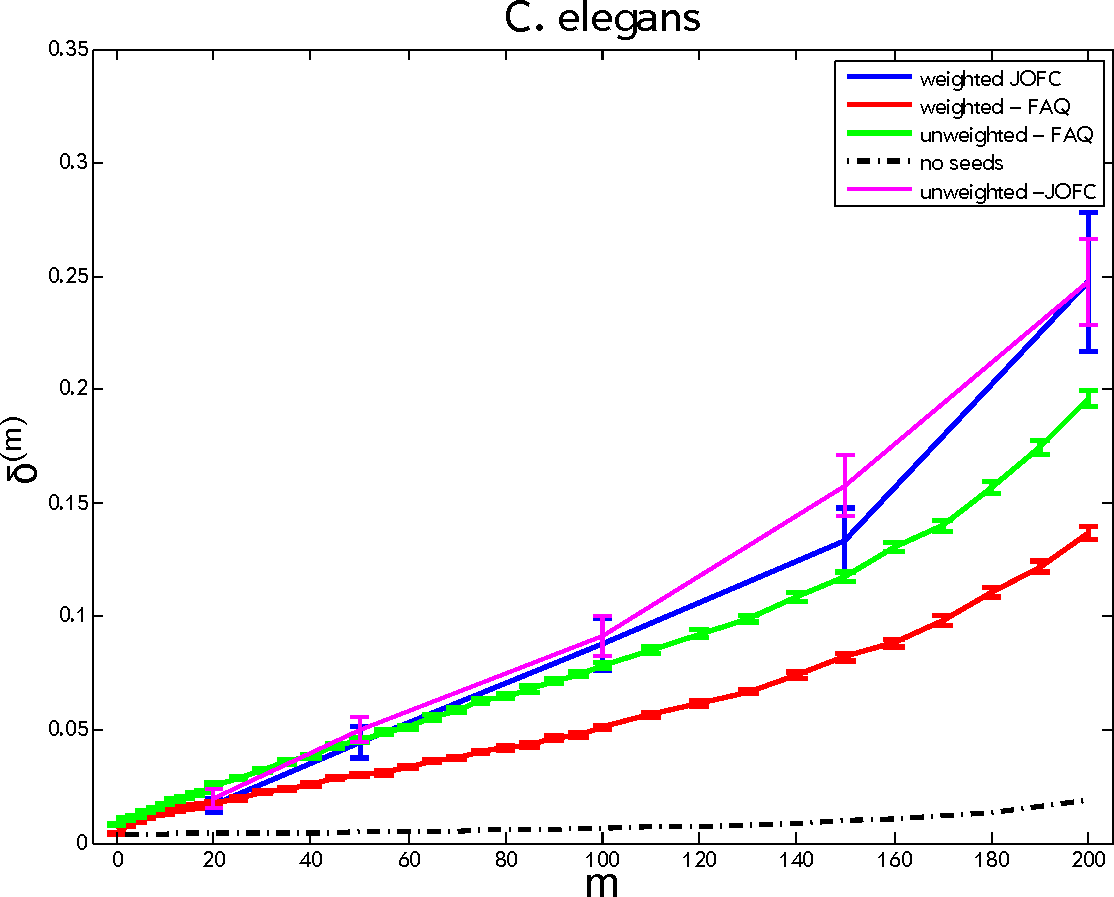
\includegraphics[scale=0.75]{worm_jofc_vs_faq_wt_unwt-crop}
\caption{Graph Matching experiments on the C. elegans connectomes using JOFC and FAQ algorithms \label{worm_graphmatch}}
\end{figure}

\subsubsection{Enron communication graph}
The Enron communication graph is extracted from the  Enron  email corpus, which was made public during criminal investigations by the  Federal Energy Regulatory Commission. Though the number of actual users is about 150,  each email alias is considered as a vertex in the communication graph. The original number of email aliases is 184. The whole time interval is divided into 187 sub-intervals. The emails are grouped according to which time interval their timestamps are in. We then construct a time series of graphs $\mathfrak{G}=\{G^{(t)} = (V,E^{(t)})\}$ where $E^{(t)}$ correspond to emails that were sent at $t^{th}$ interval. We are interested in the intervals $t=130$  and $t=131$. When isolated vertices (and their corresponding vertices in the other graph) are removed in these two graphs  , the number of vertices is reduced to 146. It is these two pruned graphs we match.

\begin{figure}
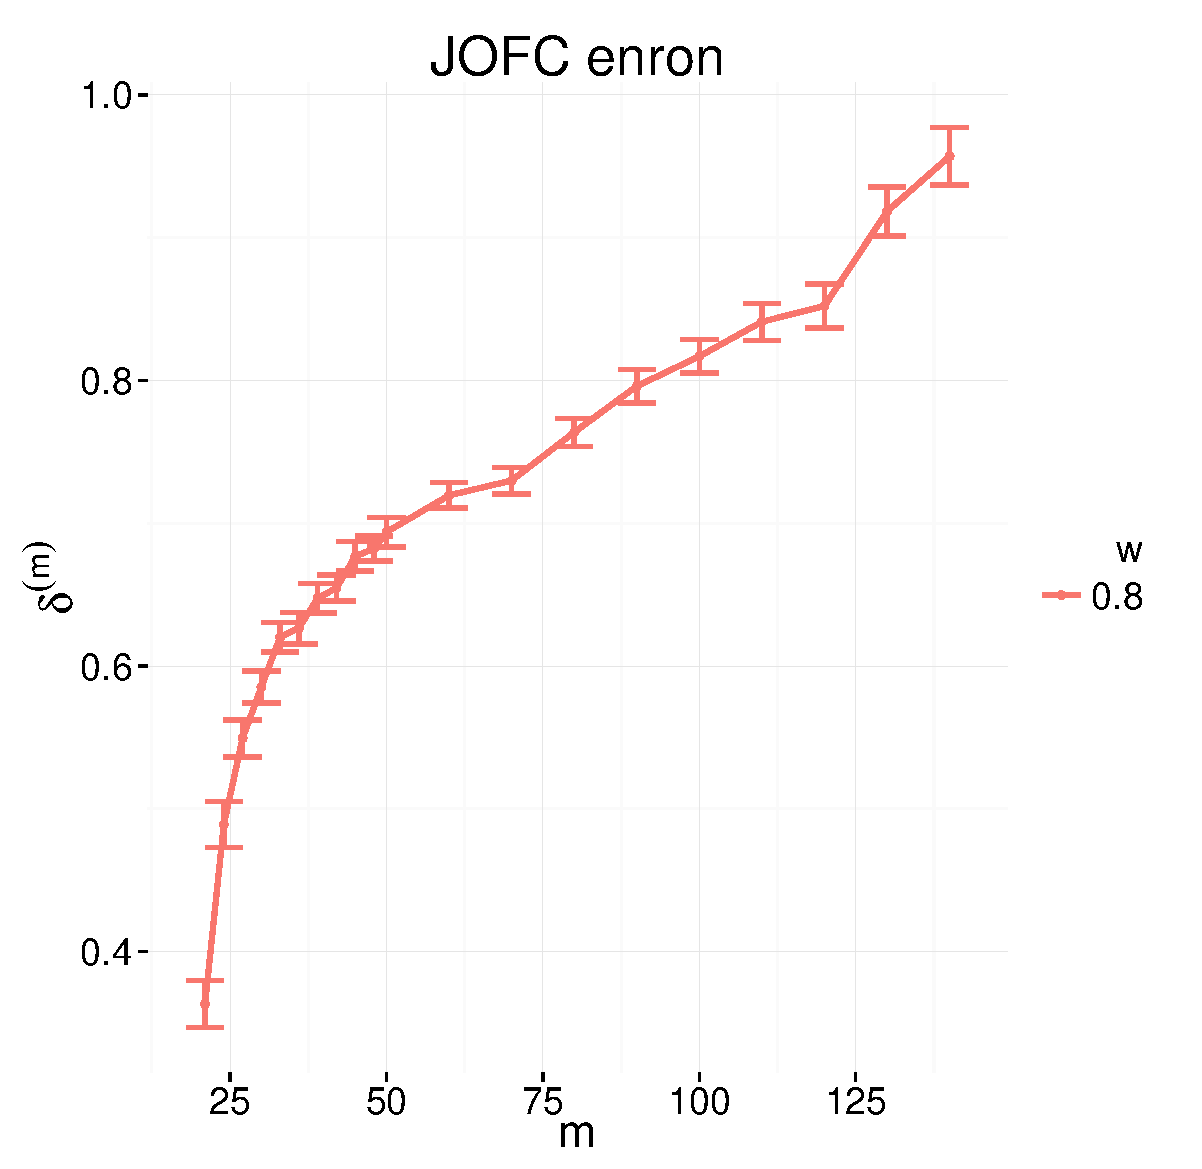
\includegraphics[scale=0.75]{JOFC-enron_dim_20}
\caption{Experiments on the Enron communication graphs for JOFC \label{enron_graphmatch}}
\end{figure}

\begin{figure}
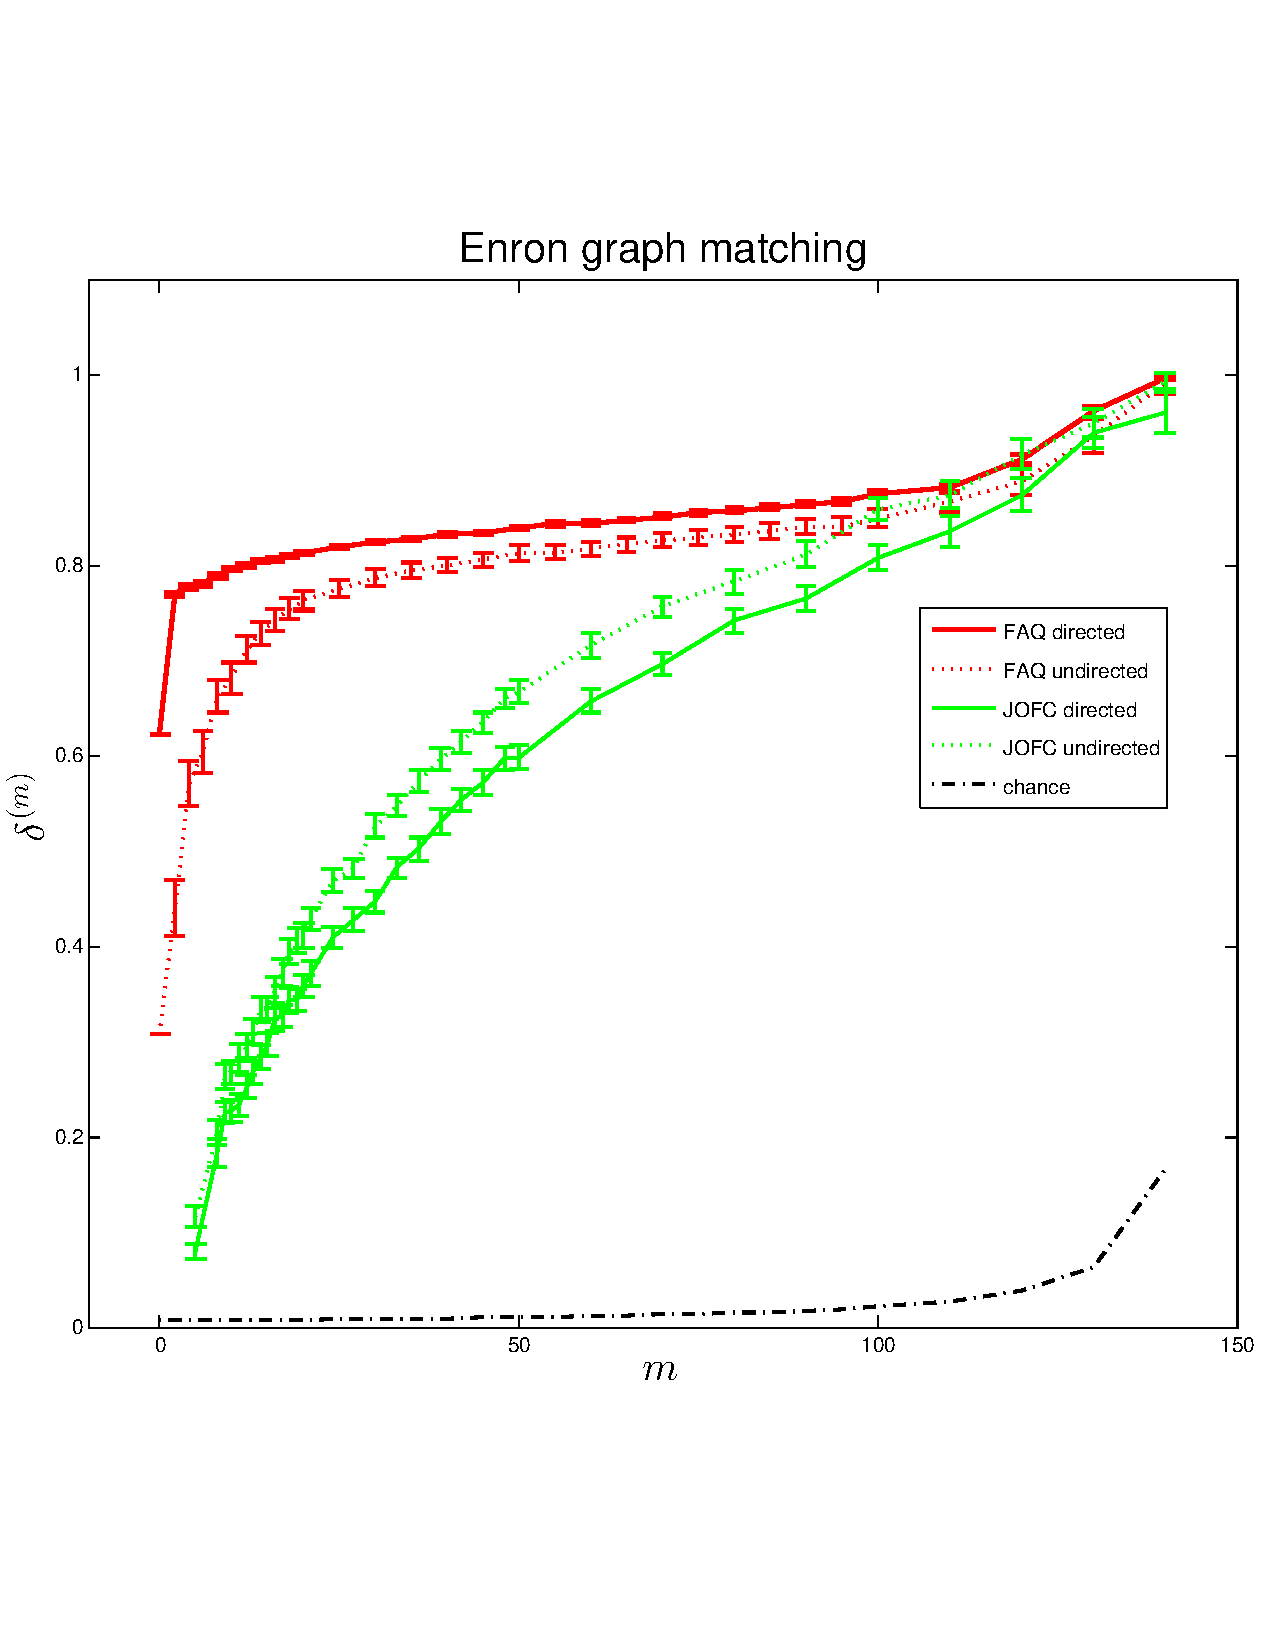
\includegraphics[scale=0.75]{enron-JOFC-FAQ-paper.pdf}
\caption{Experiments on the Enron communication graphs for FAQ and JOFC \label{enron_graphmatch_faq_jofc}}
\end{figure}

\subsubsection{Wikipedia hyperlink subgraph}

To test the JOFC approach with real data, a collection of articles are collected from the English Wikipedia, consisting of the
 directed 2-neighborhood of the document "Algebraic Geometry". 
   This  collection of 1382 articles and the correspondence of each article in French 
Wikipedia is our real-life dataset. It is possible to utilize both textual content of the documents and the hyperlink graph structure. The textual content of the documents is summarized by the bag-of-words model. Dissimilarities between documents  in the same language are computed by the Lin-Pantel discounted mutual information \cite{LinPantel,PantelLin}
 and cosine dissimilarity $k(x_{ik}; x_{jk}) = 1 - (x_{ik} x_{jk})/(\|x_{ik}\|_2\|x_{ik}\|_2)$. 
 The dissimilarities based on the hyperlink graph of the collection of the articles are 
 for each pair of vertices $i$ and $j$, the number of vertices one must travel to go from $i$ to $j$.  Further details about this dataset is available in \cite{Zhiliang_disparate}.

\begin{figure}
\includegraphics[scale=0.75]{wiki-all-with-unseeded.pdf}
\caption{Graph Matching Experiments on the English and French Wikipedia subgraph for FAQ \label{wiki_graphmatch}}
\end{figure}
      
\subsubsection{Charitynet graph}

The charitynet dataset consists  of timestamped donation relationships between 8052 donors and 756 charities. The donations are divided into two time intervals according to whether they are before the midpoint of the earliest and latest timestamps.
Let $tmid = \frac{(tmax - tmin)}{2}$.
We build two bipartite graphs represented by $B_1$ and $B_2$ for $\left[tmin,tmid\right)$ and $\left(tmid,tmax\right]$, respectively --
each $B^{(t)}$ is $n \times m$, where $n$ is total number of donors in all of charitynet and $m$ is total number of charities in all of charitynet.
so $B_{ij}^{(t)}$ is a 1 if donor $i$ gives to charity $j$ during time interval $t$.

For charities $i$ and $j$,
let $A_{ij}^{(t)}= \sum_{k}{(B_{ik}^{(t)}B_{jk}^{(t)}}$, i.e. the number of donors that both $i$ and $j$ receive from during time interval $t$.
We match the two graphs represented by  $A^{\left[tmin,tmid\right)}$, $A^{\left(tmid,tmax\right]}$.
\begin{figure}
\includegraphics[scale=0.4]{charitynet_SGM_JOFCvsFAQ}
\caption{Graph Matching experiments on the two Charitynet graphs for JOFC \label{charitynet_graphmatch}}
\end{figure}

\subsection{1-to-k matching of vertices} 

Consider the case where the correspondences between vertices in $A$ and $B$ are not one-to-one. We consider a very simple case where 
the $i^{th}$ vertex in $B$ corresponds to $k_i$ vertices in $A$ where $1\leq k_i \leq k_{max}$ where $k_{max}$ is the maximum number of corresponding vertices a $B$ vertex can have.  Denote by $g$ the correspondence function from vertices in $G_1$ to vertices in $G_2$. Given $r$ vertices in $B$, and the corresponding vertices in $V_1$ for each of the $r$ vertices ($u \in V_1$ such that $g(u)=v_2$), the task is  to find at most $k_max$ closest matches to each vertex of of $B$. 
The three information retrieval performance measures are used: Precision, Recall and F-measure.

$$\mathrm{Precision} =\frac{\textrm{Number of correct matches found}}{\textrm{Number of found matches}}$$
$$\mathrm{Recall}    =\frac{\textrm{Number of correct matches found}}{\textrm{Number of true matches}}$$

$$F-measure  =\frac{2 \times \textrm{Precision} \times \textrm{Recall}}{\textrm{Precision} + \textrm{Recall}}$$

For each vertex of $B$, the number of true matches is $k_i$. The three performance measure is calculated for each vertex of $B$ and then the three averages over all vertices $B$ is the performance measures computed for the  matching.

\begin{figure}
\includegraphics[scale=0.65]{Total_precision_JOFC_1_to_k_match_paper.pdf}
\caption{Graph Matching experiments on simulated graphs for JOFC \label{1_k_graphmatch_sim}}
\end{figure}



%<<'child-chapter12_Grassmannian.Rnw', child='chapter12_Grassmannian.Rnw',eval=TRUE>>=
%@


\include{appendix}

%% REFERENCES

% if you use BIBTEX
\bibliographystyle{IEEEtran}
\bibliography{priebe-thesis-JOFC}
% 
% \begin{vita}
% 
% \begin{wrapfigure}{l}{0pt}
% \includegraphics[width=2in,height=2.5in,clip,keepaspectratio]{rjvheadshot}
% \end{wrapfigure}
% 
% 
% 
% \end{vita}
\end{document}
